	\newpage
\section{Podręcznik użytkownika}  %6
%Opis jak używać programu. Mogą być z zrzut ekranu razem z opisem. 


\subsection{Wyszukiwanie i uruchomienie aplikacji Ttest} 

\hspace{0.60cm}Pierwszym krokiem jaki musimy podjąć, aby uruchomić aplikację, jest włączenie telefonu a następnie wyszukujemy po nazwie aplikację: Ttest. Powinno nam wyskoczyć okienko z nazwą i ikonką. Rysunek \ref{rys:ikona_6} przedstawia efekt po wyszukaniu aplikacji Ttest.

\begin{figure}[!hbt]
	\begin{center}
		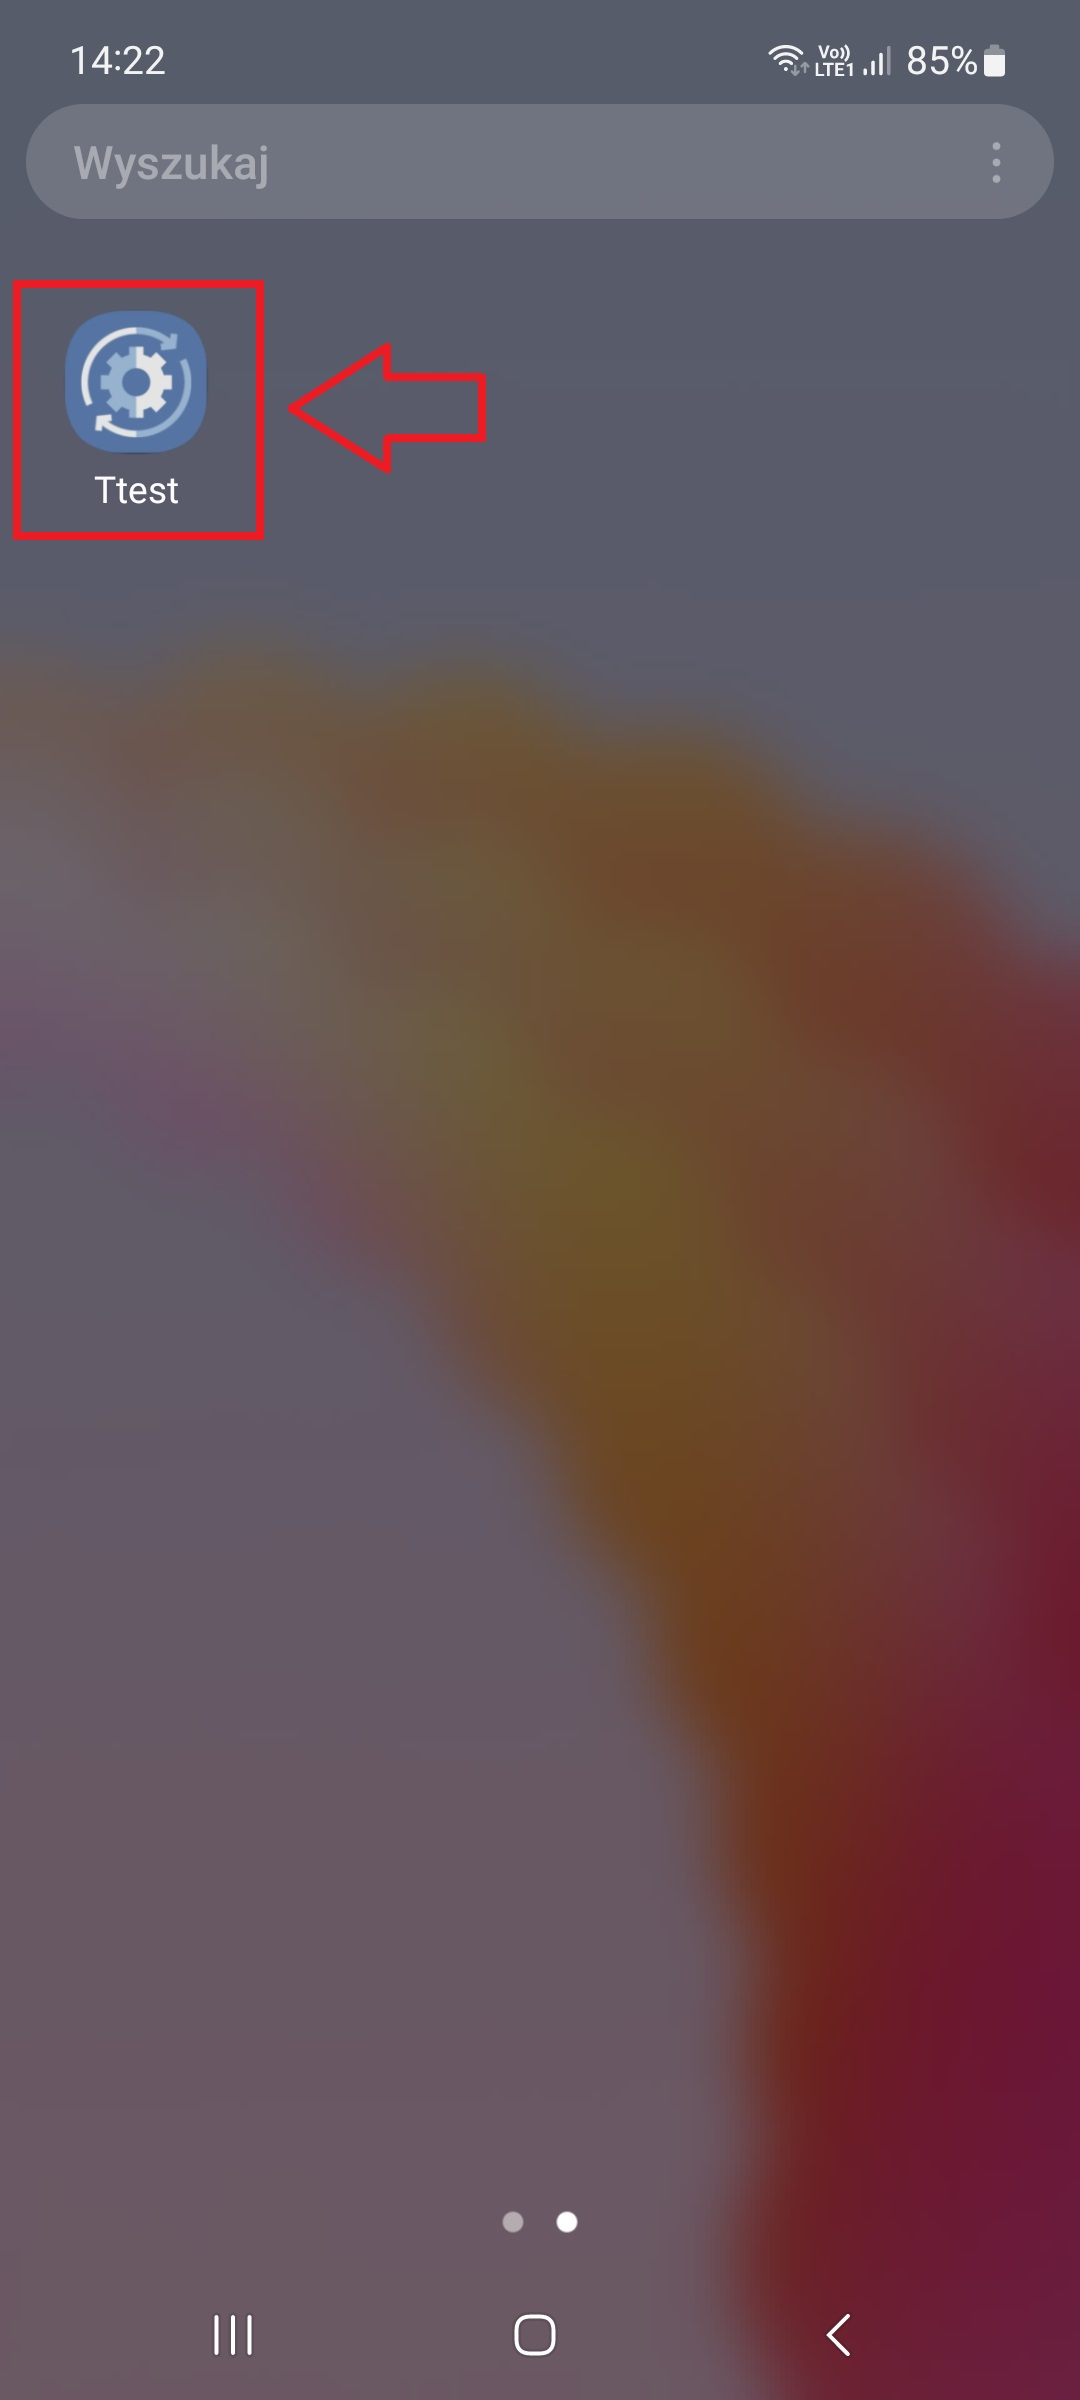
\includegraphics[angle=360, width=0.45\textwidth]{rys/punkt6/ikona.jpg}
		\caption{Wyszukiwanie aplikacji}
		\label{rys:ikona_6}
	\end{center}
\end{figure}

Gdy już odnaleźliśmy aplikację Ttest, klikamy w nią a program automatycznie przekierowuję nas do menu głównego aplikacji. 

\newpage


Menu składa się z ośmiu różnych testów. Są to testy: latarki, trybu ciemnego, czujnika zbliżeniowego, lokalizacji, wifi, dźwięku, mikrofonu oraz aparatu. Każdy jeden z testów kryję się pod przyciskiem, który został ówcześnie oznaczony odpowiednią grafiką odpowiadającą danemu testowi oraz podpisem znajdującym się u dołu obrazka. Na samym dole pod testami znajduję się przycisk z napisem "Wyniki", jest to swego rodzaju podsumowanie działalności wszystkich testów znajdujących się \\ w aplikacji. Rysunek \ref{rys:menu1} prezentuje widok menu głównego.

\begin{figure}[!hbt]
	\begin{center}
		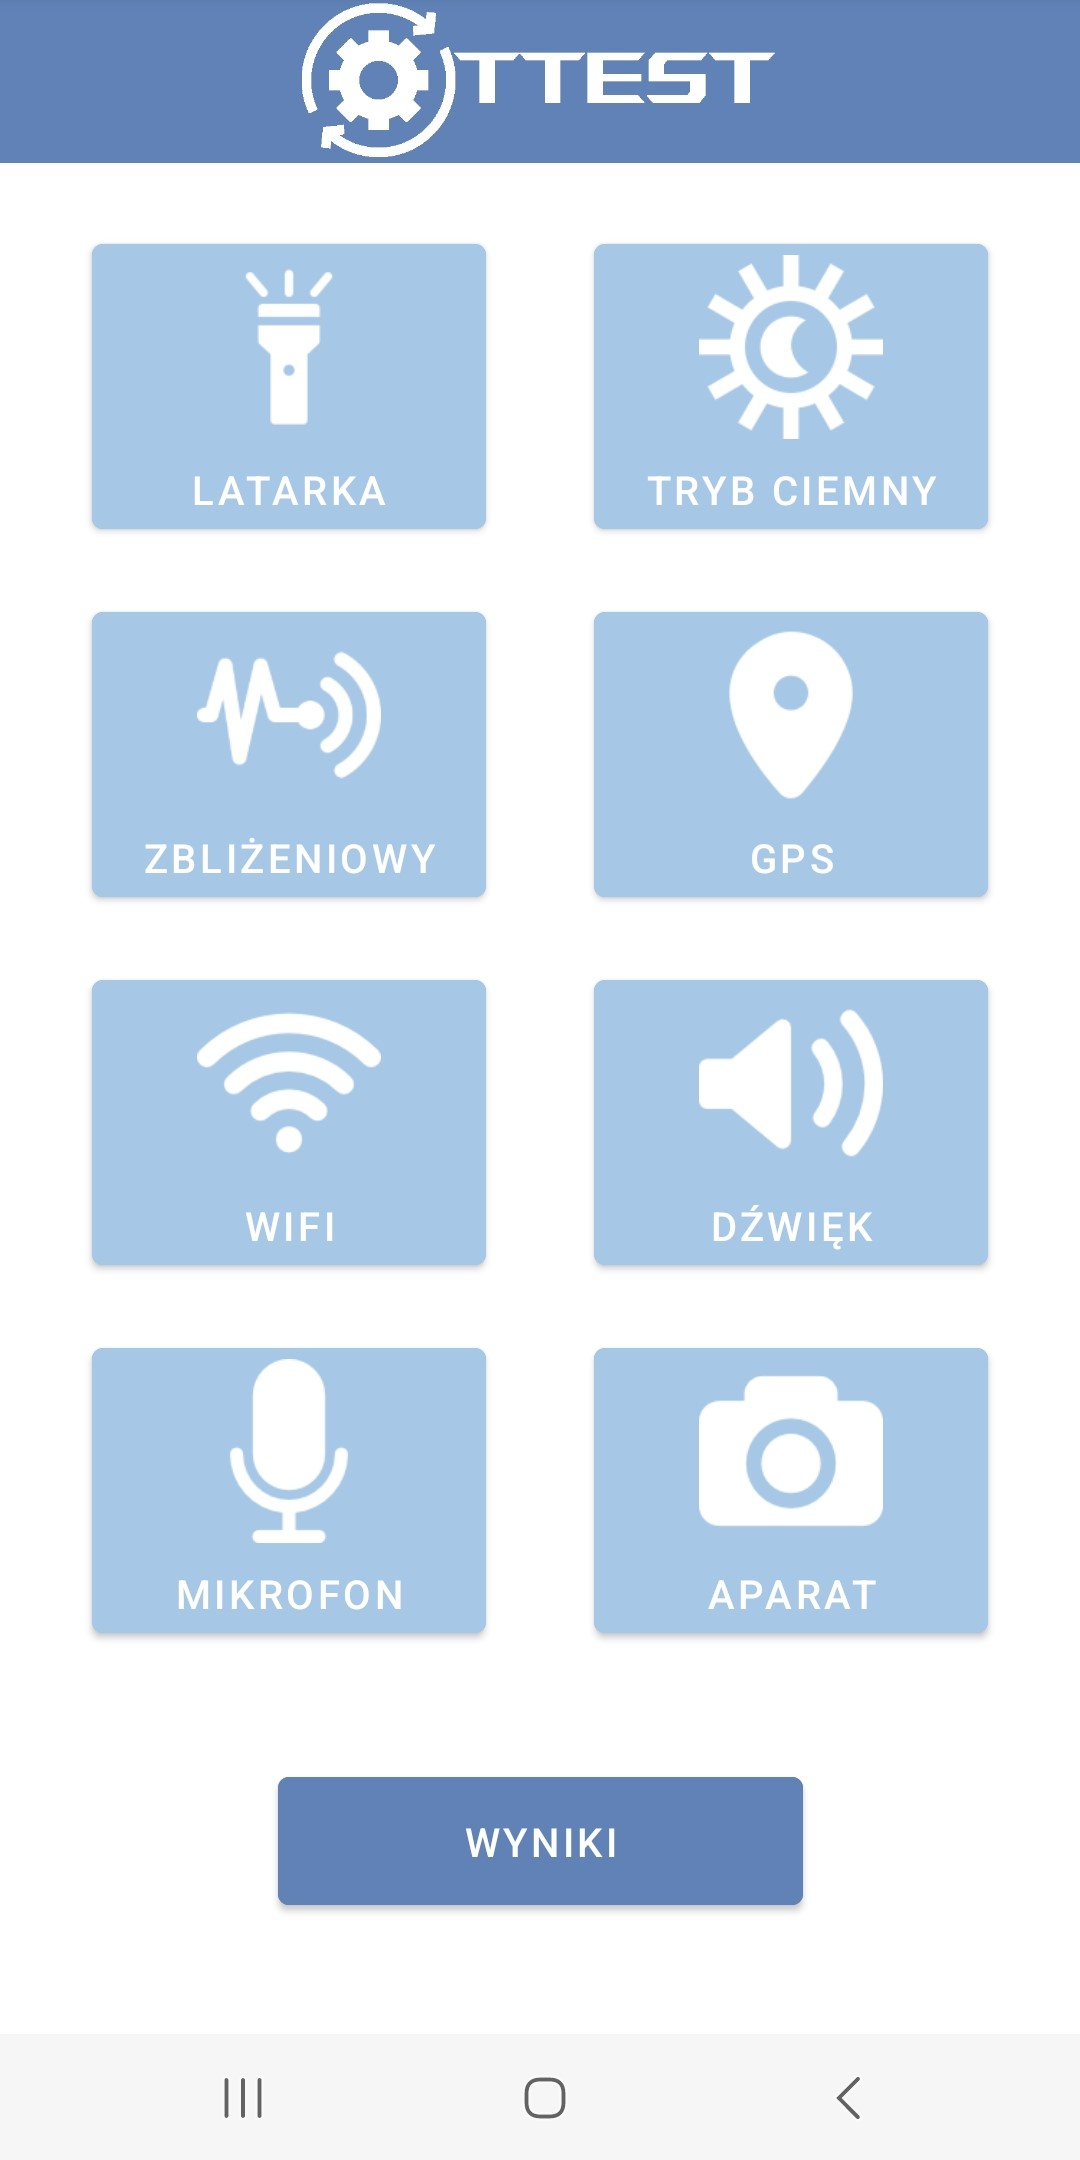
\includegraphics[angle=360, width=0.45\textwidth]{rys/punkt6/menu1.jpg}
		\caption{Menu główne}
		\label{rys:menu1}
	\end{center}
\end{figure}

\newpage


\subsection{Test latarki} 

\hspace{0.60cm}Aby uruchomić latarkę w menu głównego wybieramy i klikamy na ikonkę latarki, która znajduję się na samej górze po lewej stronie. Rysunek \ref{rys:latarka1} ukazuję kafelek który należy wybrać. 

\begin{figure}[!hbt]
	\begin{center}
		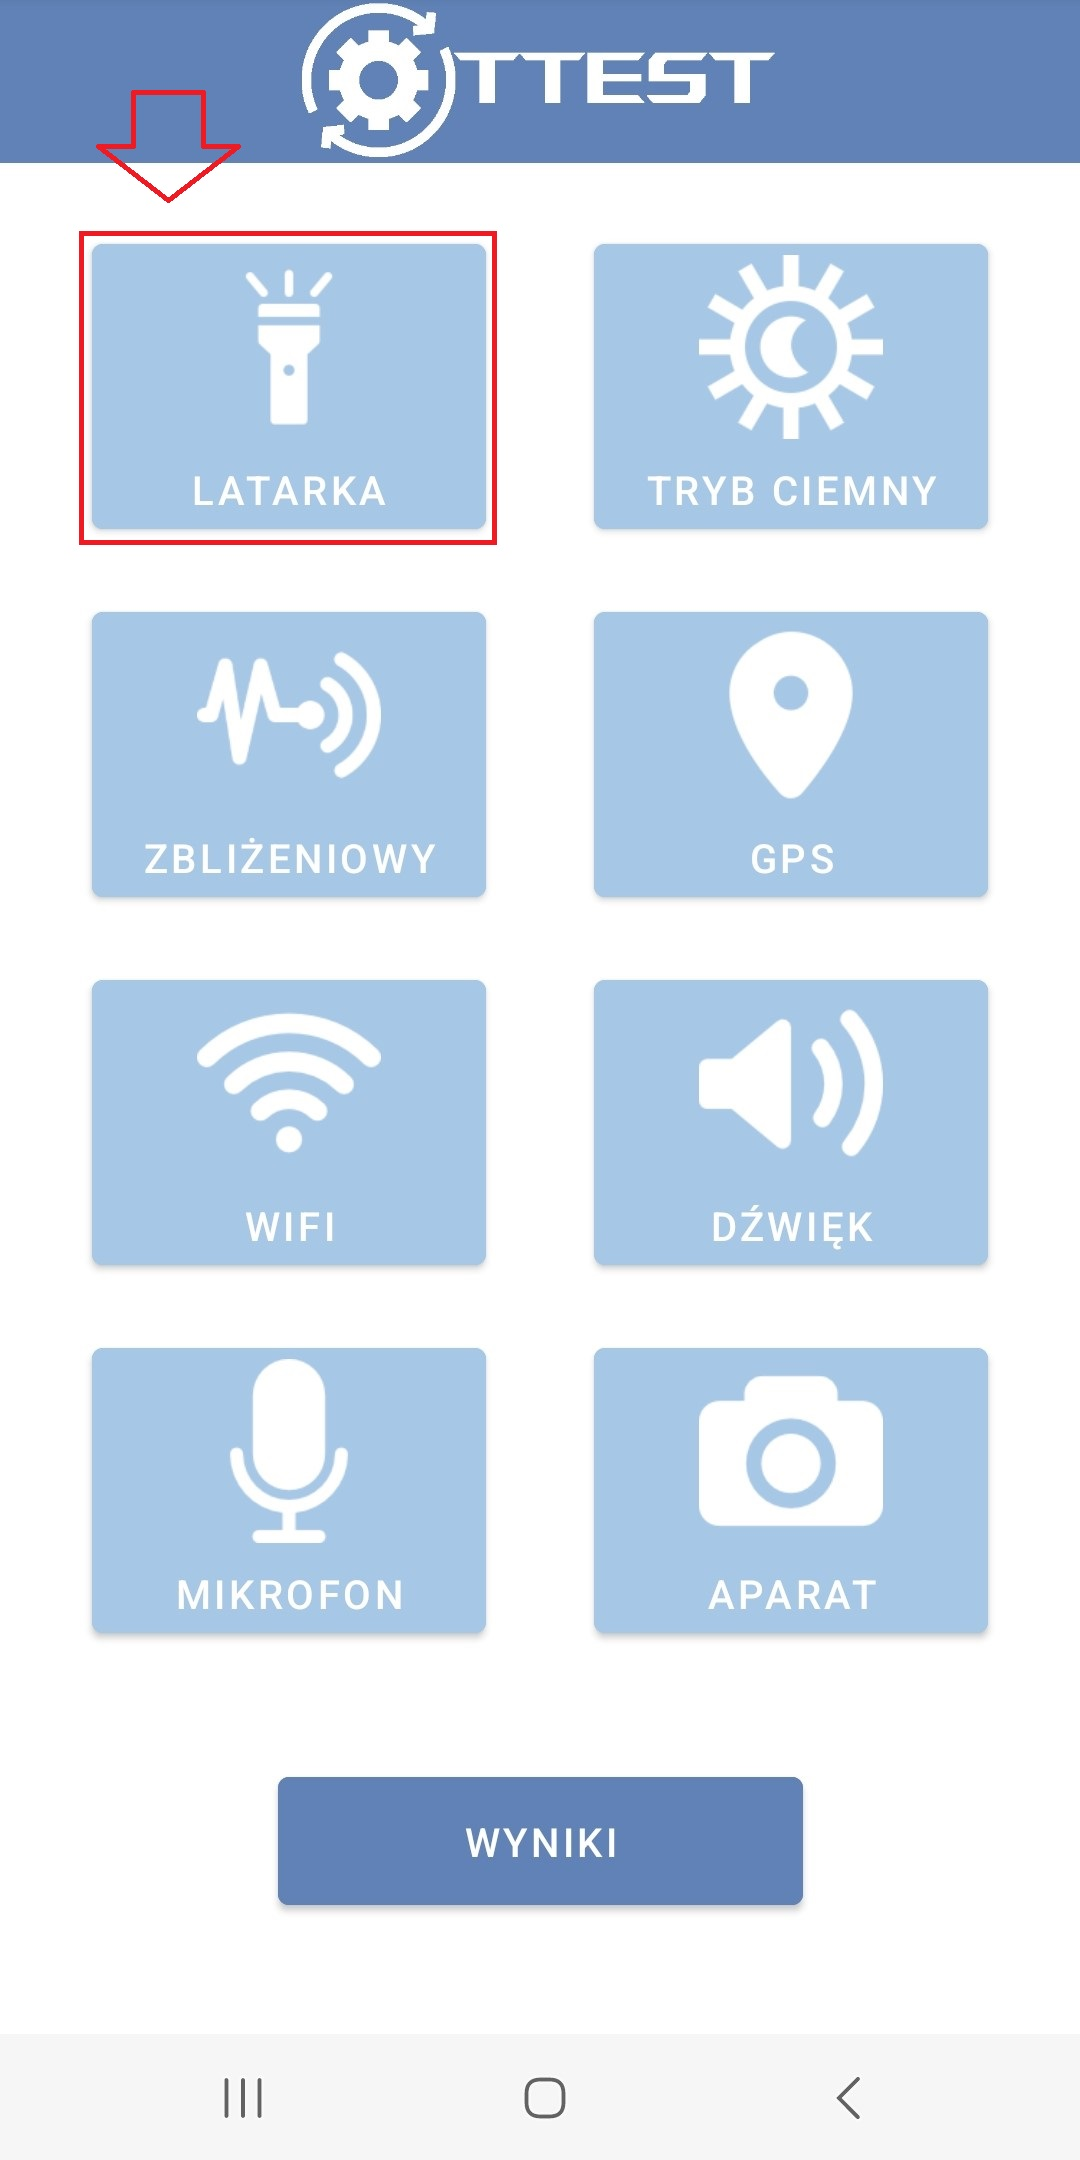
\includegraphics[angle=360, width=0.45\textwidth]{rys/punkt6/latarka1.jpg}
		\caption{Wybór latarki}
		\label{rys:latarka1}
	\end{center}
\end{figure}

Następnie aplikacja przekierowuje nas do testu latarki. Pojawia się okienko \\ a na środku znajduję się grafika przedstawiająca latarkę.
Gdy naciśniemy na latarkę jej kolor zmieni się z szarego na zielony, oznacza to że test przeszedł pomyślnie \\ i latarka włączyła się. Oprócz zielonego koloru pod latarką wyświetla się komunikat informujący nas o tym że latarka została włączona. Rysunek \ref{rys:latarka2} przedstawia zrzut ekranu potwierdzający pomyślny przebieg testu.
\newpage


\begin{figure}[!hbt]
	\begin{center}
		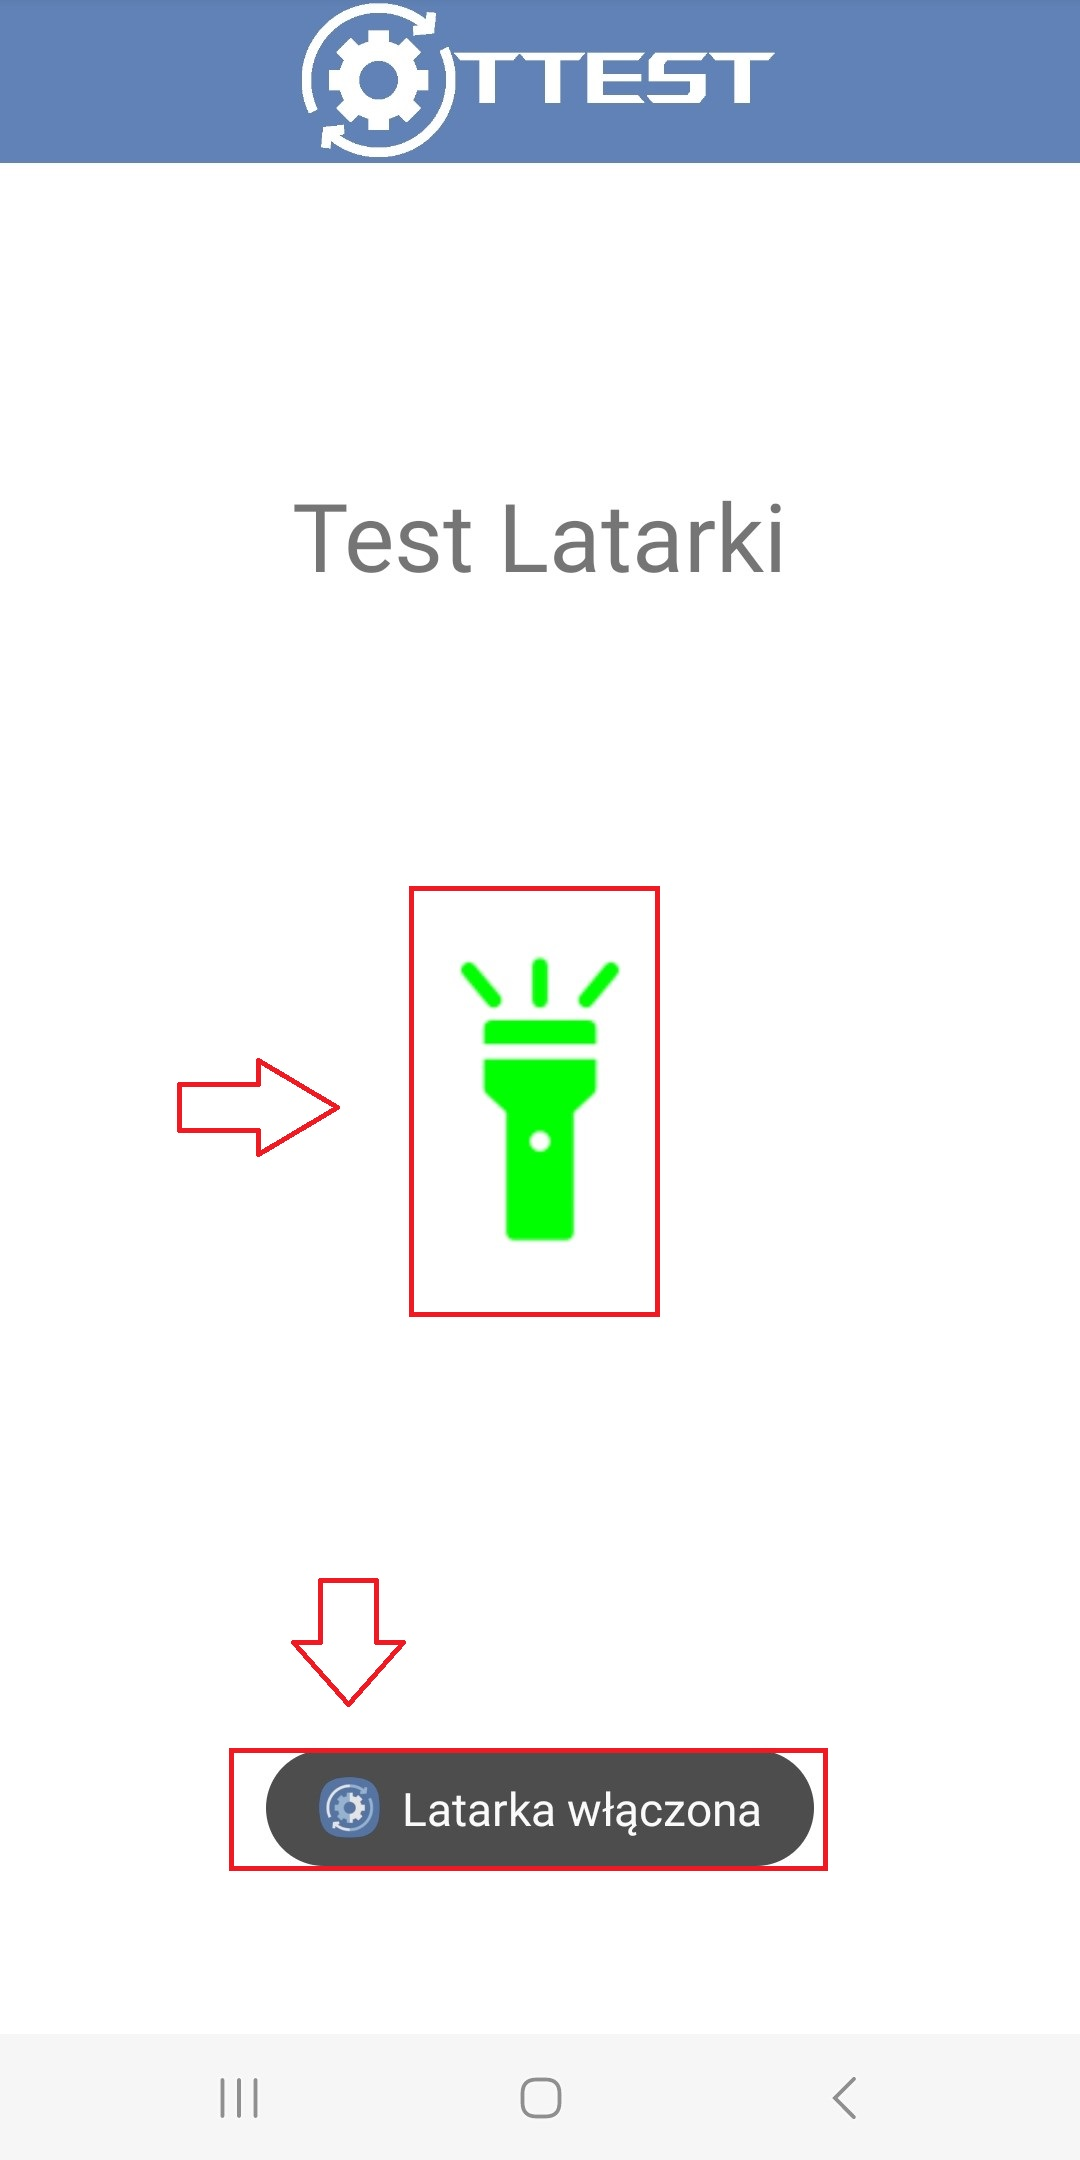
\includegraphics[angle=360, width=0.31\textwidth]{rys/punkt6/latarka2.jpg}
		\caption{Włączenie latarki}
		\label{rys:latarka2}
	\end{center}
\end{figure}

Analogicznie jak w przypadku włączenia gdy naciśniemy na latarkę kolejny raz, test zostanie przerwany, latarka wyłączy się i zmieni kolor z zielonego na czerwony. Rysunek \ref{rys:latarka3} przedstawia wyłączoną latarkę.

\begin{figure}[!hbt]
	\begin{center}
		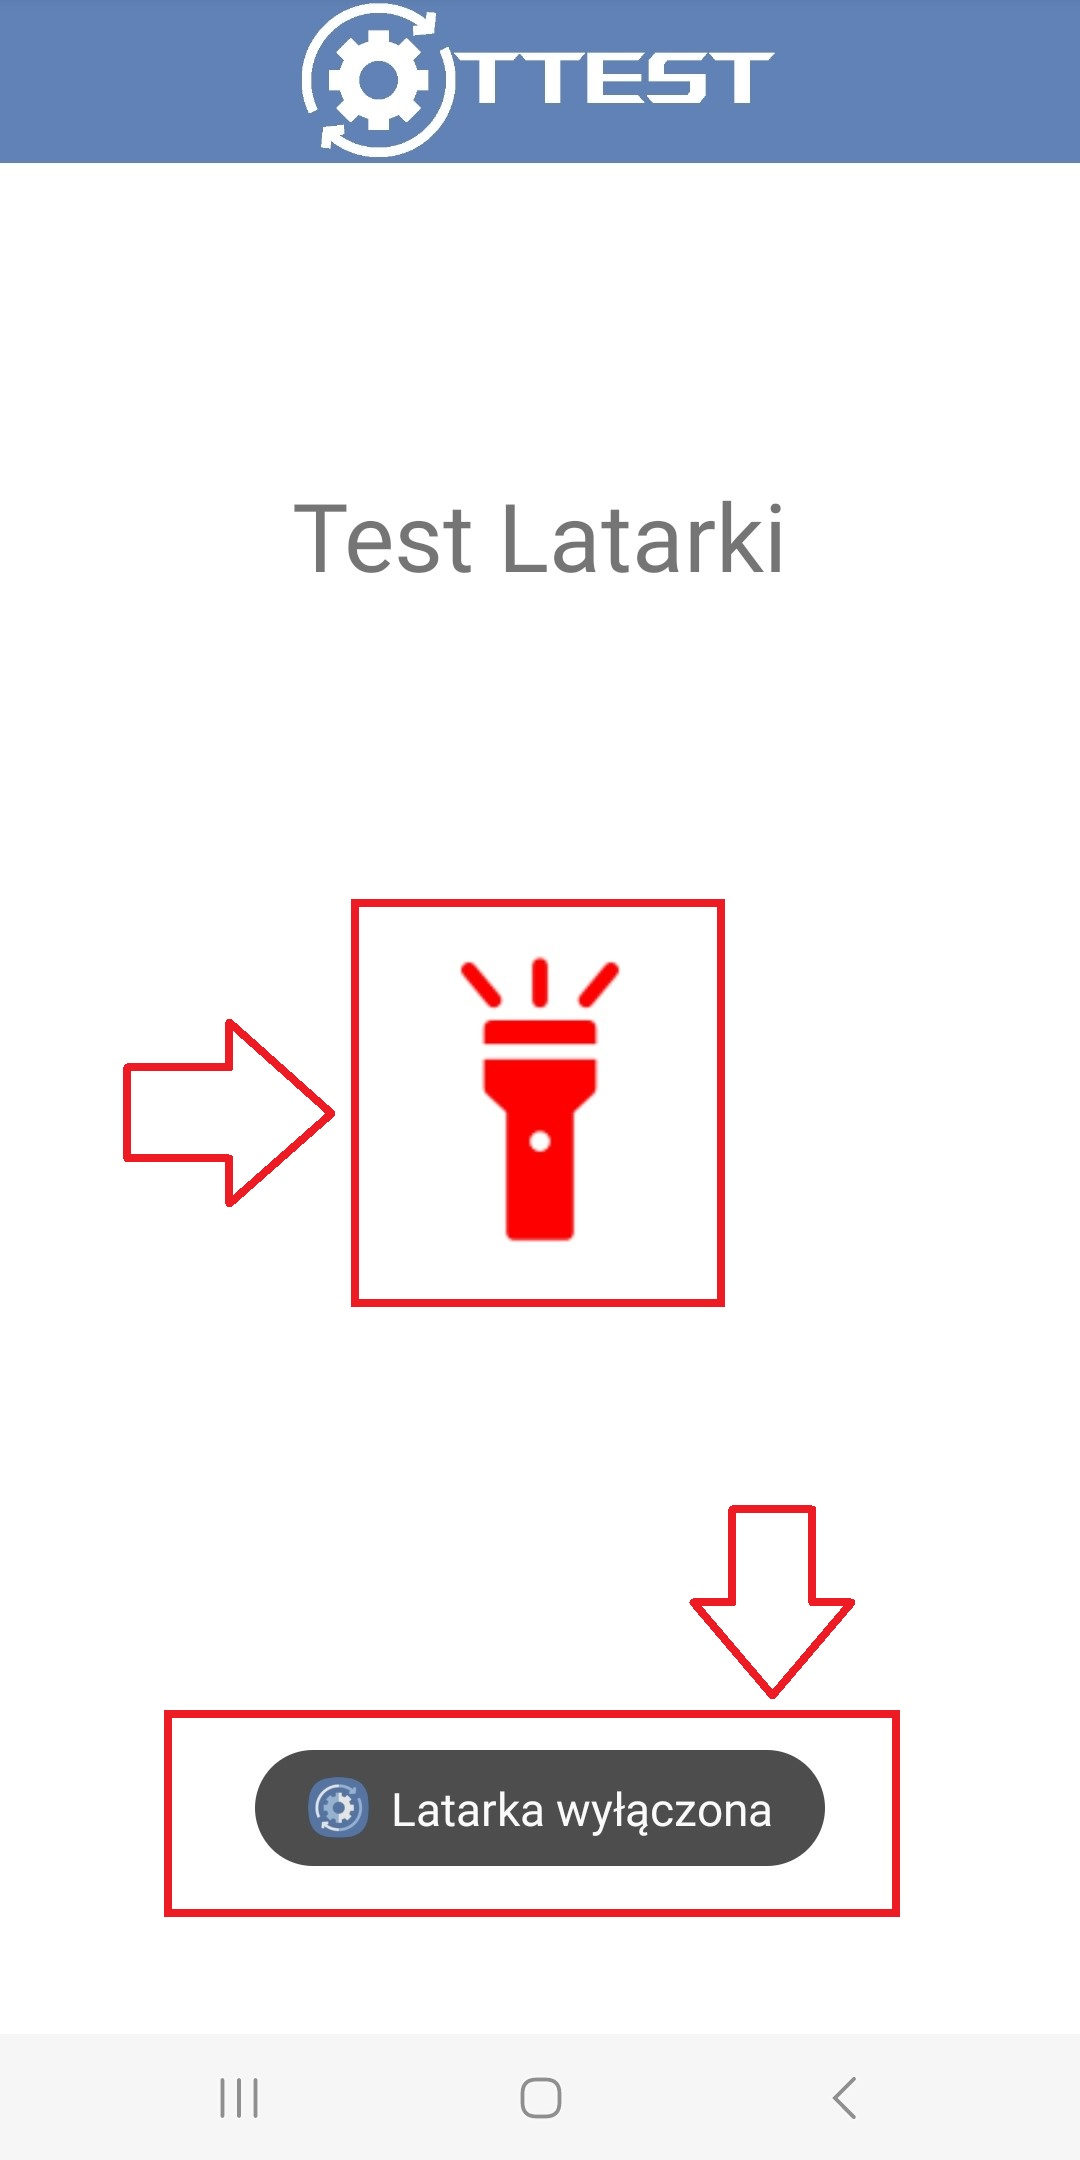
\includegraphics[angle=360, width=0.31\textwidth]{rys/punkt6/latarka3.jpg}
		\caption{Wyłączenie latarki}
		\label{rys:latarka3}
	\end{center}
\end{figure}

\newpage


\subsection{Test trybu ciemnego}

\hspace{0.60cm}Aby uruchomić tryb ciemny musimy na panelu głównym wybrać i kliknąć \\ w ikonkę który znajduję się na samej górze po prawej stronie. Rysunek \ref{rys:menu2} obrazuje kafelek który musimy wybrać i kliknąć aby przejść do testu.

\begin{figure}[!hbt]
	\begin{center}
		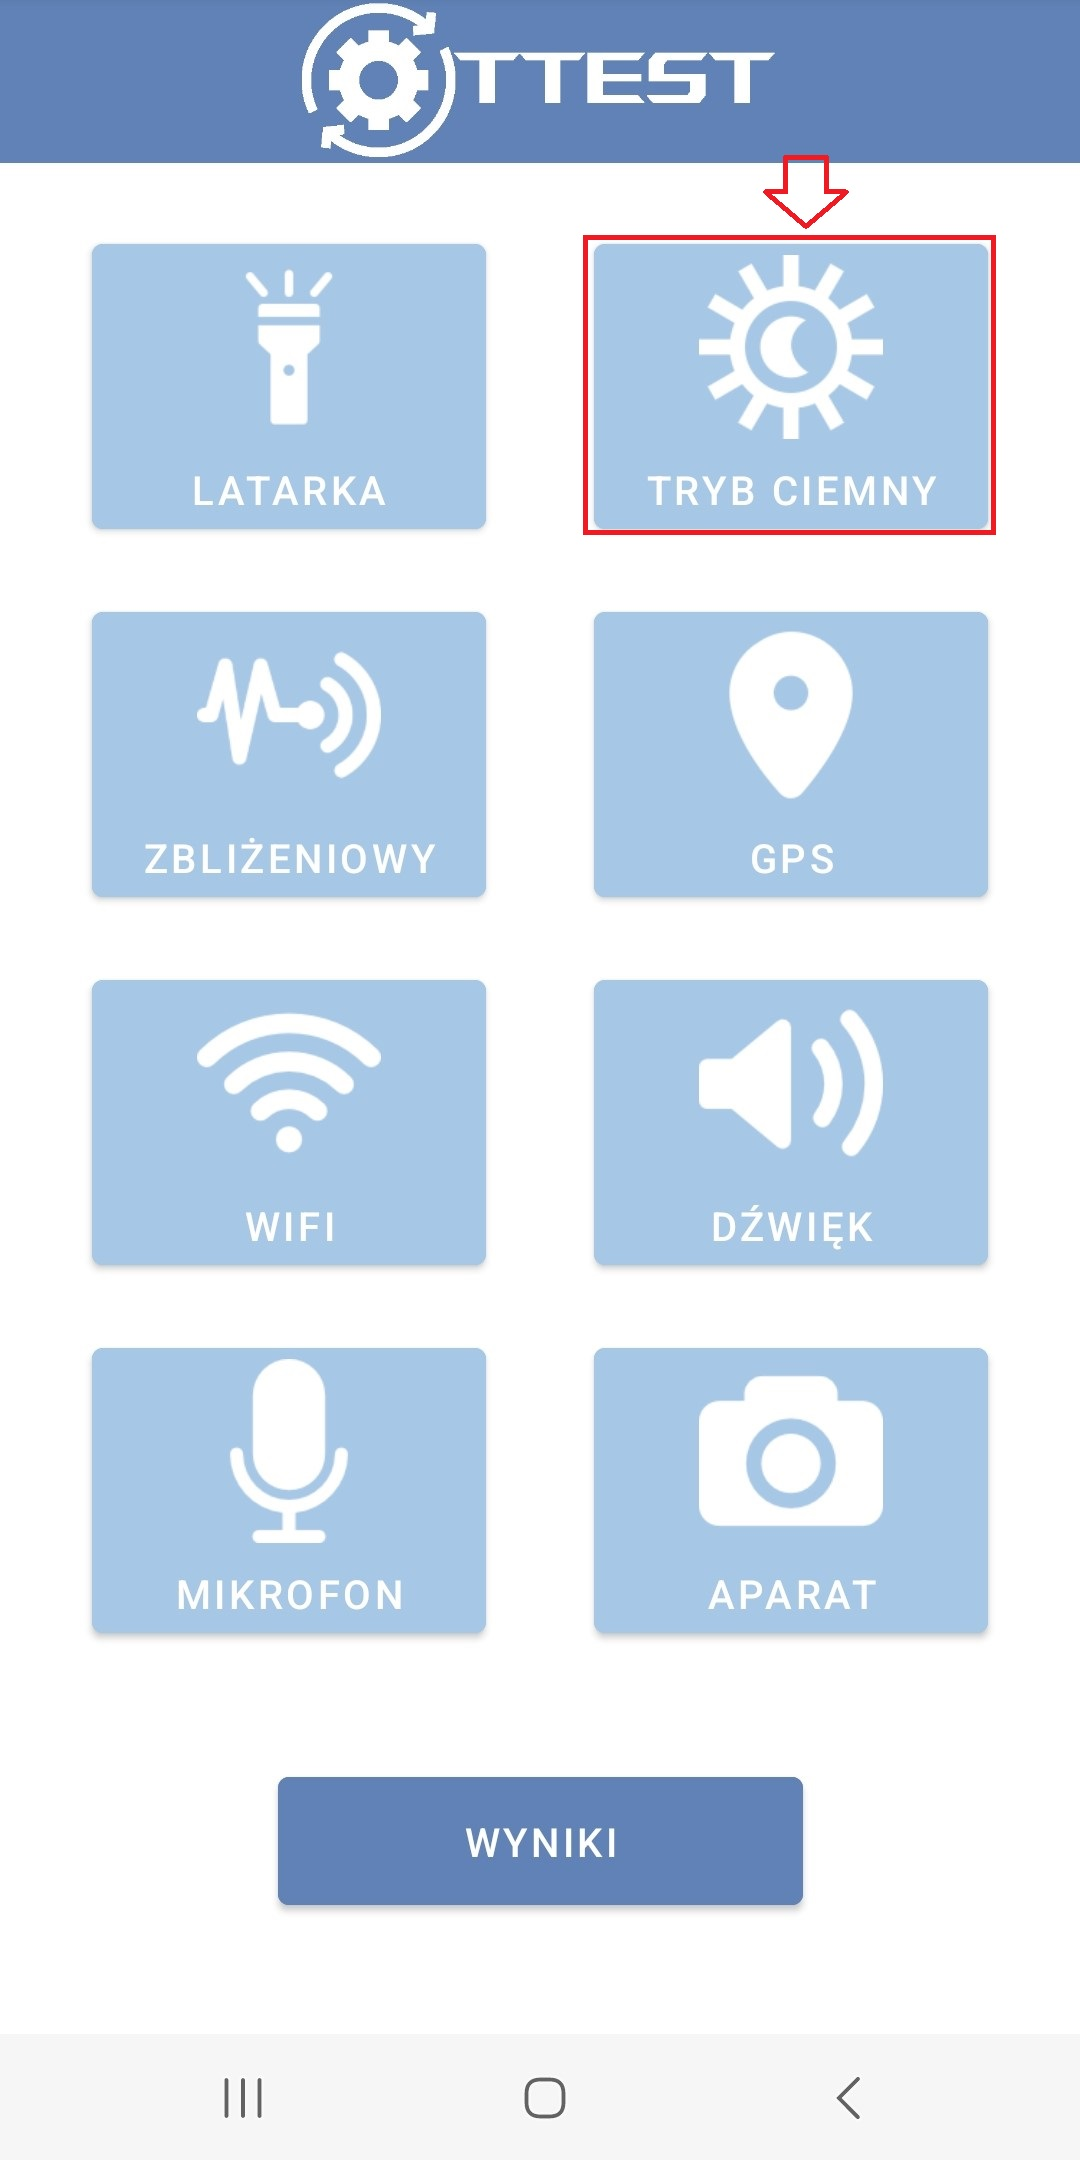
\includegraphics[angle=360, width=0.45\textwidth]{rys/punkt6/menu2.jpg}
		\caption{Wybór trybu ciemnego}
		\label{rys:menu2}
	\end{center}
\end{figure}

Następnie aplikacja przekierowuje nas do okienka testowego. Na środku znajduję się grafika, która podobnie jak w przypadku latarki zmienia kolory z zielonego na czerwony, lub odwrotnie w zależności czy tryb zostanie włączony lub wyłączony. Jeżeli klikniemy na ikonkę a jej kolor zmieni się na zielony oznacza to że test przeszedł pomyślnie, co więcej ekran zmieni kolor z białego na czarny a pod grafiką dodatkowo pojawia się informacja o tym że tryb ciemny został uruchomiony. \\
Rysunek \ref{rys:tryb ciemny} przedstawia uruchomienie trybu ciemnego.

\newpage


\begin{figure}[!hbt]
	\begin{center}
		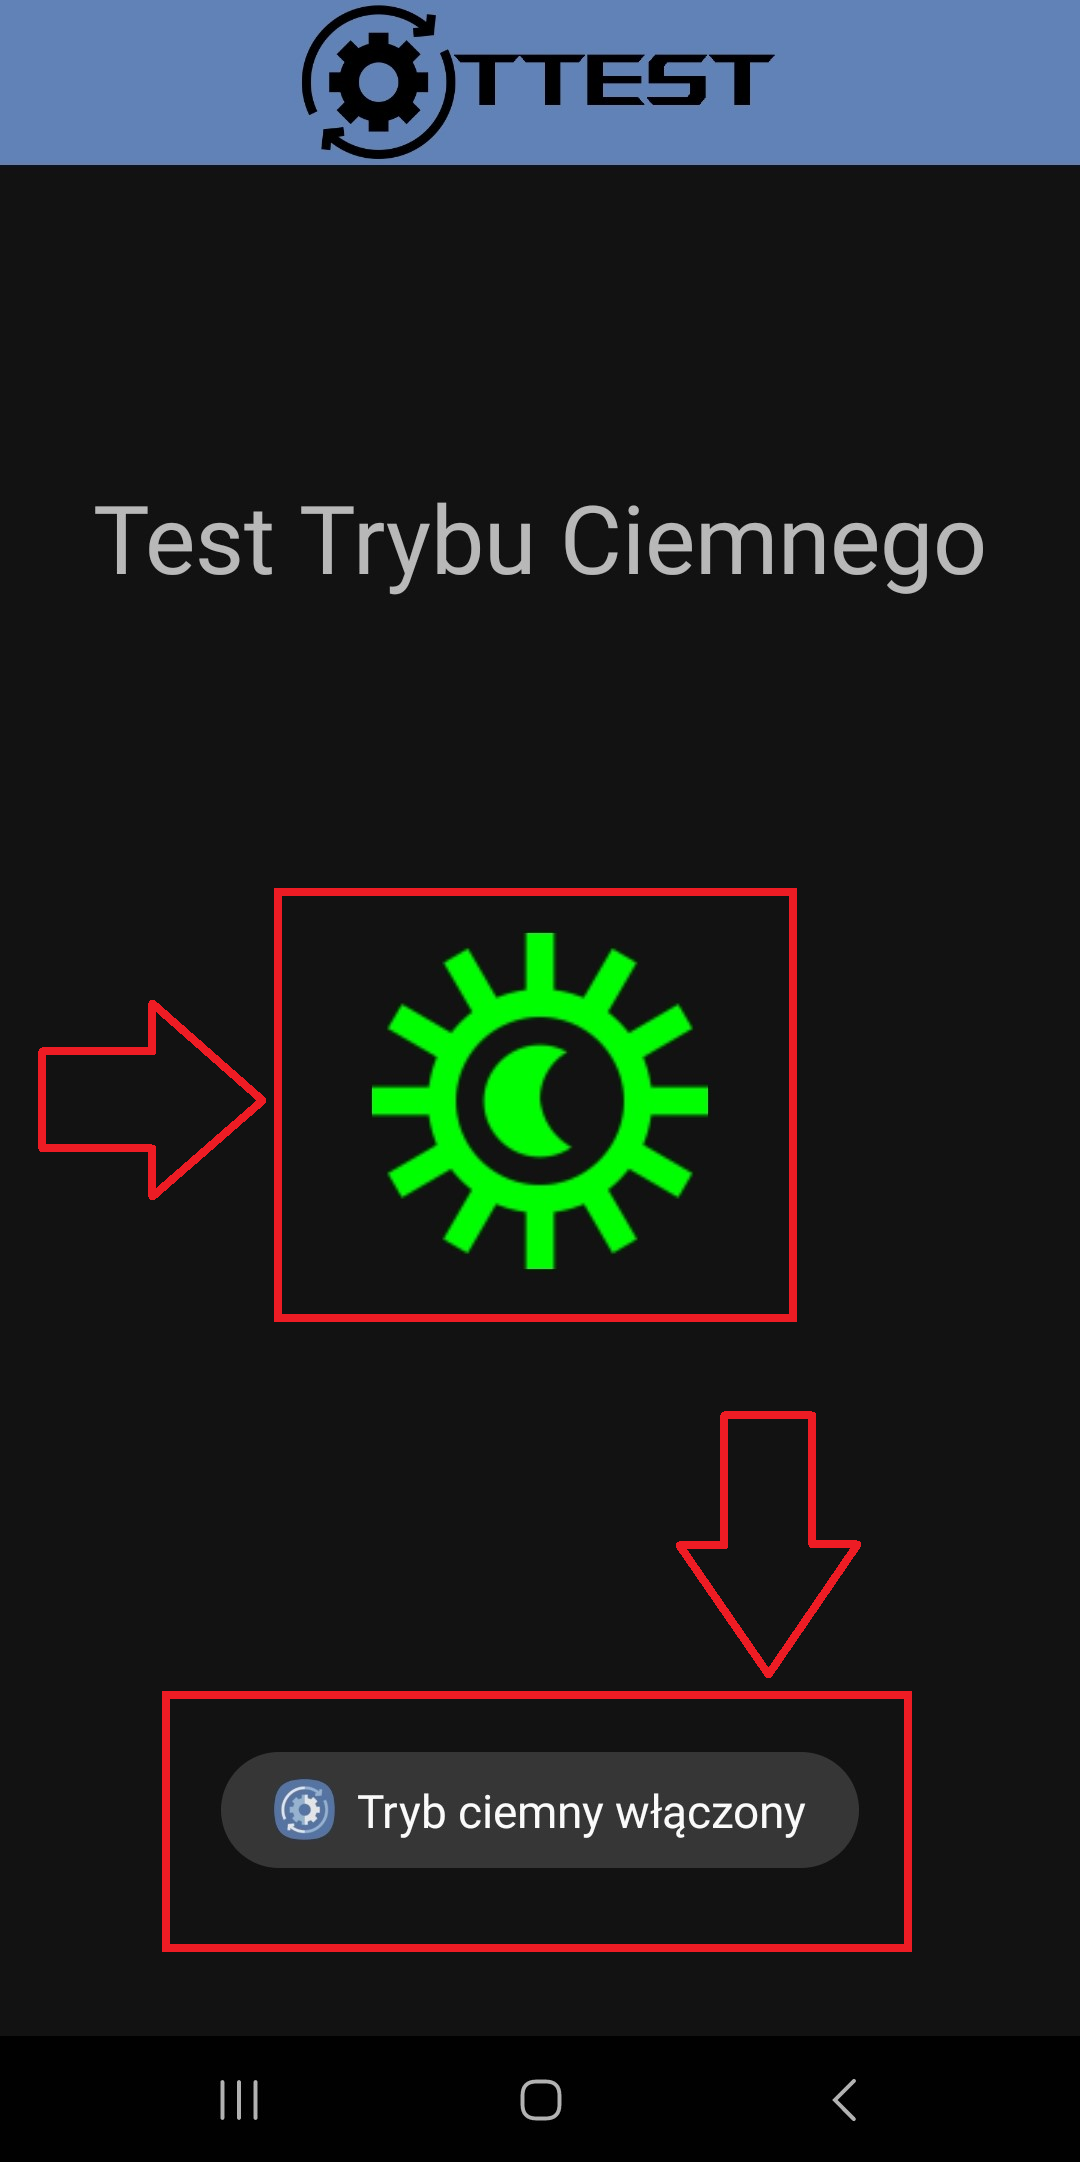
\includegraphics[angle=360, width=0.31\textwidth]{rys/punkt6/tryb ciemny.png}
		\caption{Włączenie trybu ciemnego}
		\label{rys:tryb ciemny}
	\end{center}
\end{figure}

Po kliknięciu ponownie na środkowy przycisk tryb ciemny zostaje wyłączony, kolor ikonki zmienia się na czerwony, a komunikat u dołu informuje nas o wyłączeniu trybu ciemnego. Rysunek \ref{rys:tryb ciemny1} przedstawia wyłączenie trybu ciemnego. 

\begin{figure}[!hbt]
	\begin{center}
		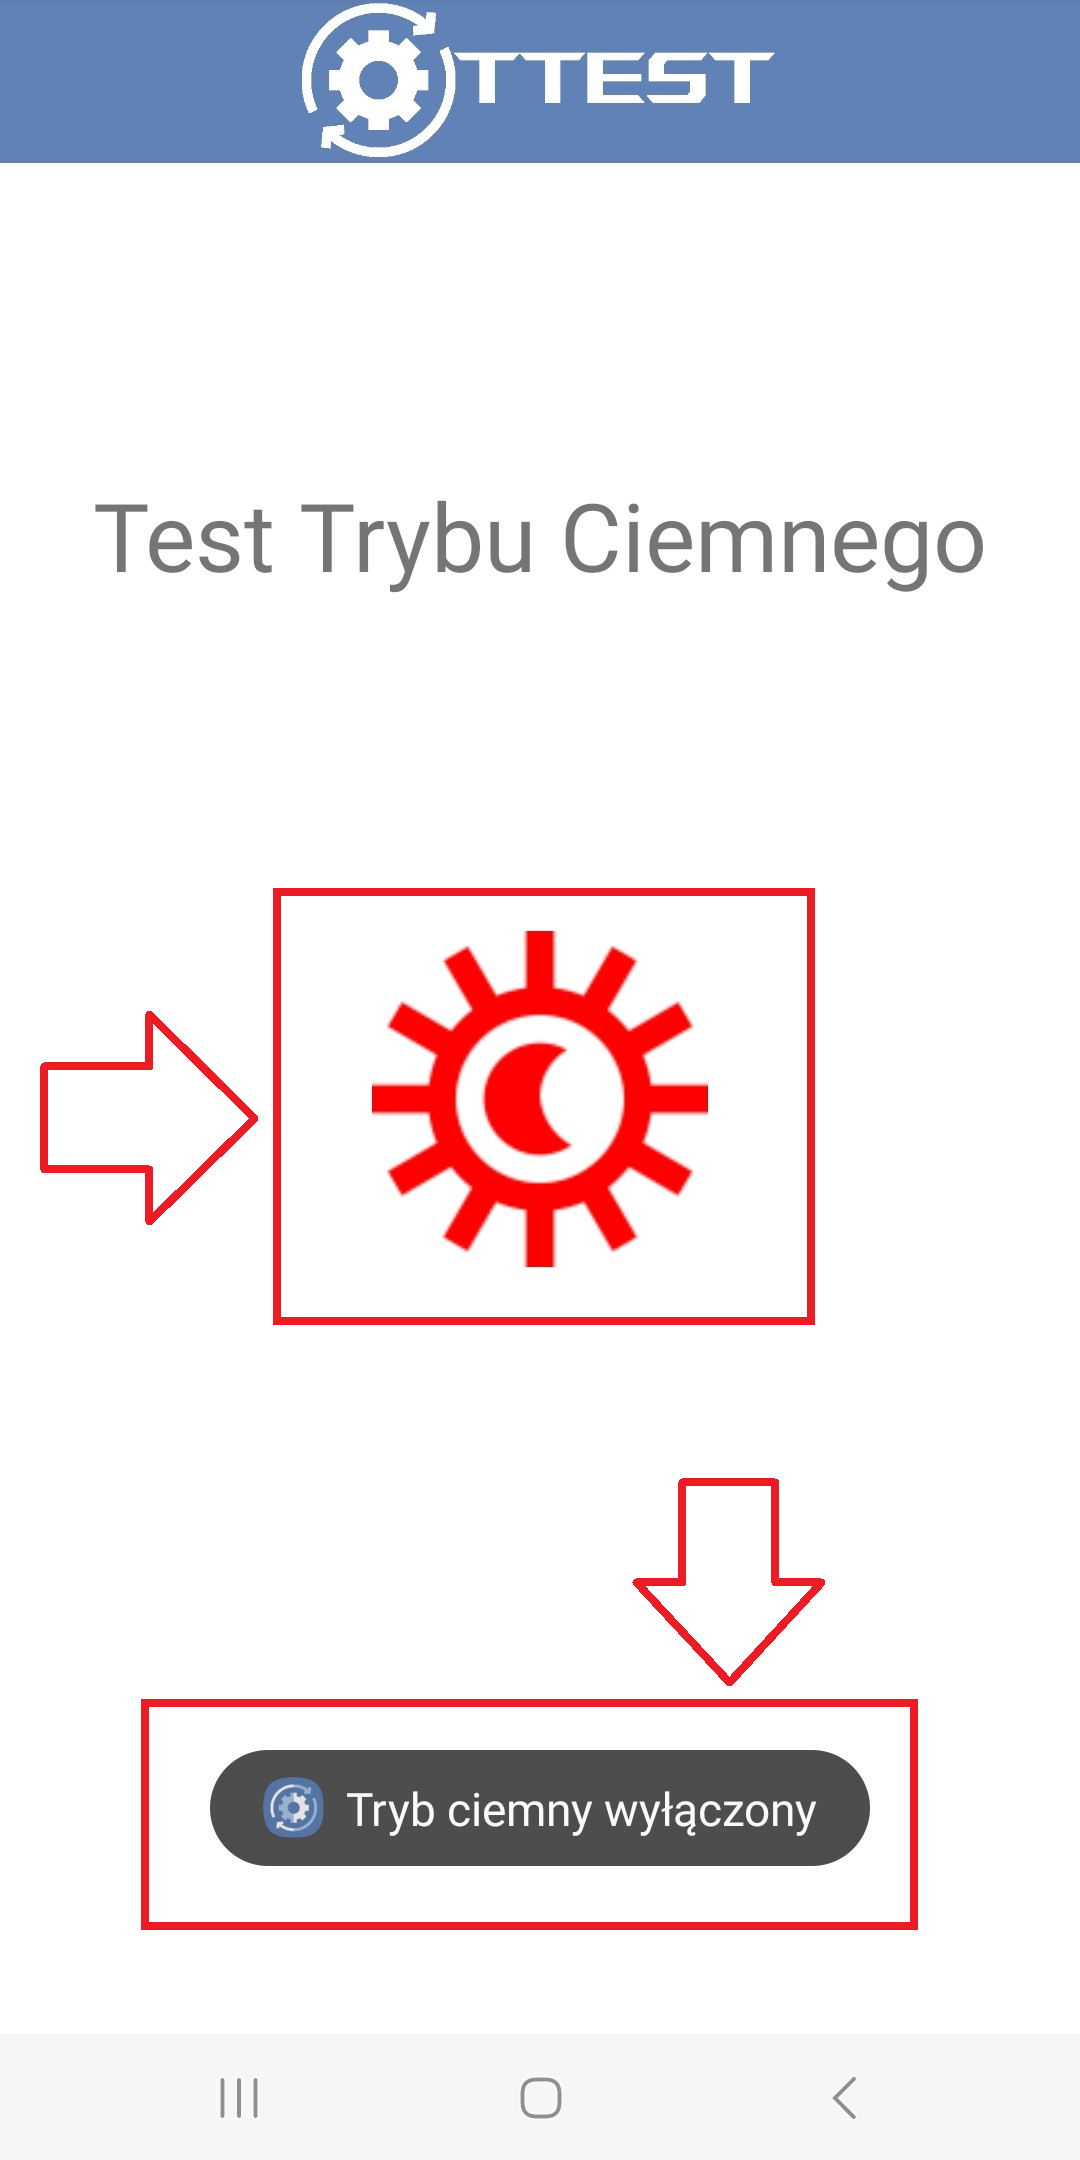
\includegraphics[angle=360, width=0.31\textwidth]{rys/punkt6/tryb ciemny1.png}
		\caption{Wyłączenie trybu ciemnego}
		\label{rys:tryb ciemny1}
	\end{center}
\end{figure}

\newpage


\subsection{Test czujnika zbliżeniowego}

\hspace{0.60cm}Aby uruchomić czujnik zbliżeniowy musimy w menu wybrać i kliknąć w ikonkę który znajduję się na pod ikonką latarki. Rysunek \ref{rys:menu3} obrazuje kafelek, który musimy wybrać i kliknąć aby przejść do testu.

\begin{figure}[!hbt]
	\begin{center}
		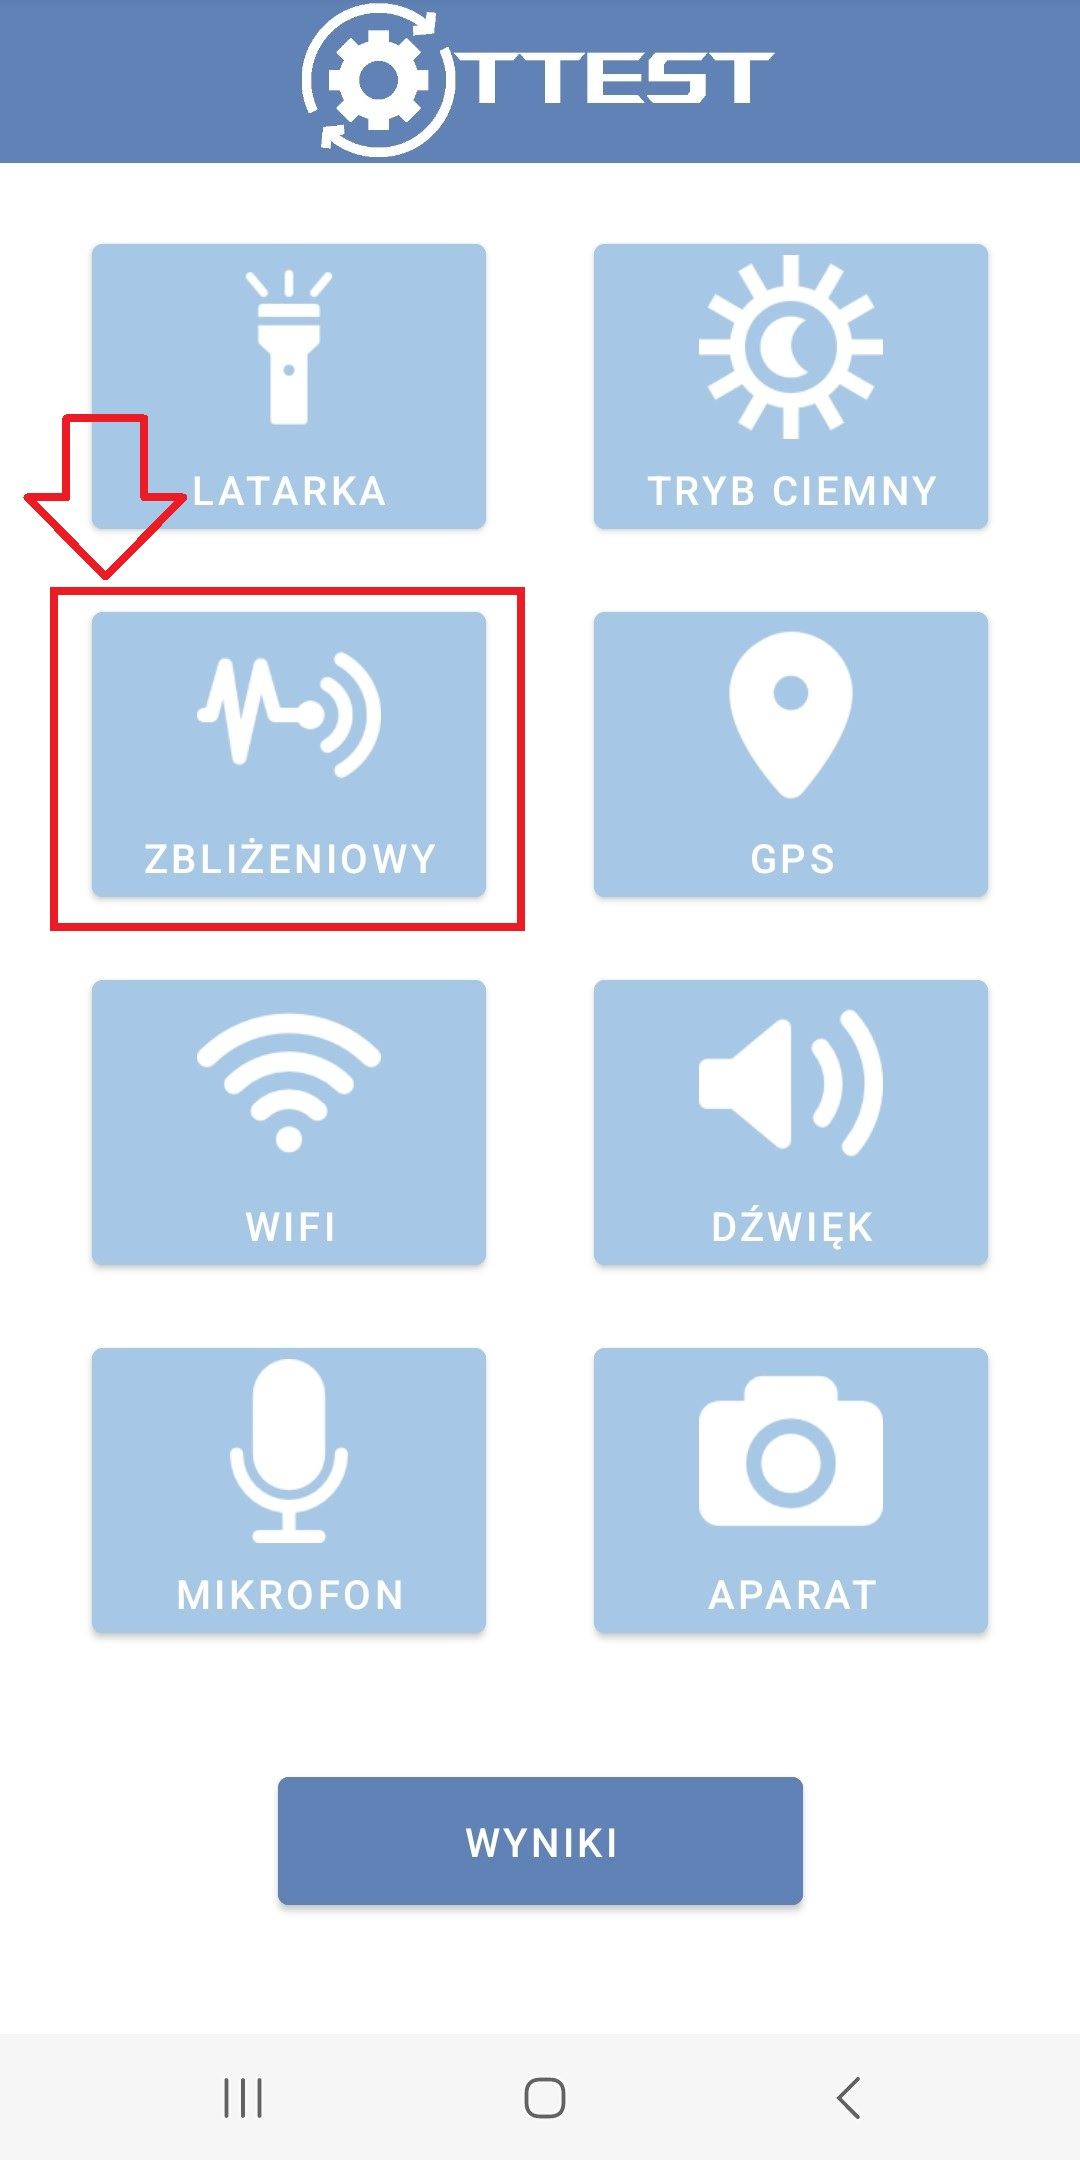
\includegraphics[angle=360, width=0.45\textwidth]{rys/punkt6/menu3.jpg}
		\caption{Lokalizacja czujnika zbliżeniowego}
		\label{rys:menu3}
	\end{center}
\end{figure}

Po przejściu do strony z testem wyświetla nam się informacja aby przyłożyć obiekt do czujnika. Rysunek \ref{rys:czujnik zbliżeniowy} prezentuje stronę z testem czujnika. \\

Czujnik znajduję się przy przedniej kamerce telefonu wystarczy przyłożyć palec a informacja zmienia się i zaczyna wyświetlać komunikat o treści : Przy czujniku jest obiekt. Jeżeli odsuniemy palec od czujnika informacja ponownie zacznie wyświetlać komunikat o treści: Przyłóż obiekt do czujnika.

\newpage


\begin{figure}[!hbt]
	\begin{center}
		\includegraphics[angle=360, width=0.32\textwidth]{rys/punkt6/czujnik zbliżeniowy}
		\caption{Strona testowa czujnika zbliżeniowego}
		\label{rys:czujnik zbliżeniowy}
	\end{center}
\end{figure}

Rysunek \ref{rys:czujnik zbliżeniowy1} przedstawia zrzut ekranu potwierdzający pomyślny przebieg testu.

\begin{figure}[!hbt]
	\begin{center}
		\includegraphics[angle=360, width=0.32\textwidth]{rys/punkt6/czujnik zbliżeniowy1}
		\caption{Działanie czujnika zbliżeniowego}
		\label{rys:czujnik zbliżeniowy1}
	\end{center}
\end{figure}

\newpage


\subsection{Test GPS}

\hspace{0.60cm}Aby uruchomić test lokalizacji musimy w menu wybrać i kliknąć w przycisk który znajduję się na pod ikonką trybu ciemnego. Rysunek \ref{rys:menu4} obrazuje kafelek, który musimy wybrać i kliknąć aby przejść do testu.

\begin{figure}[!hbt]
	\begin{center}
		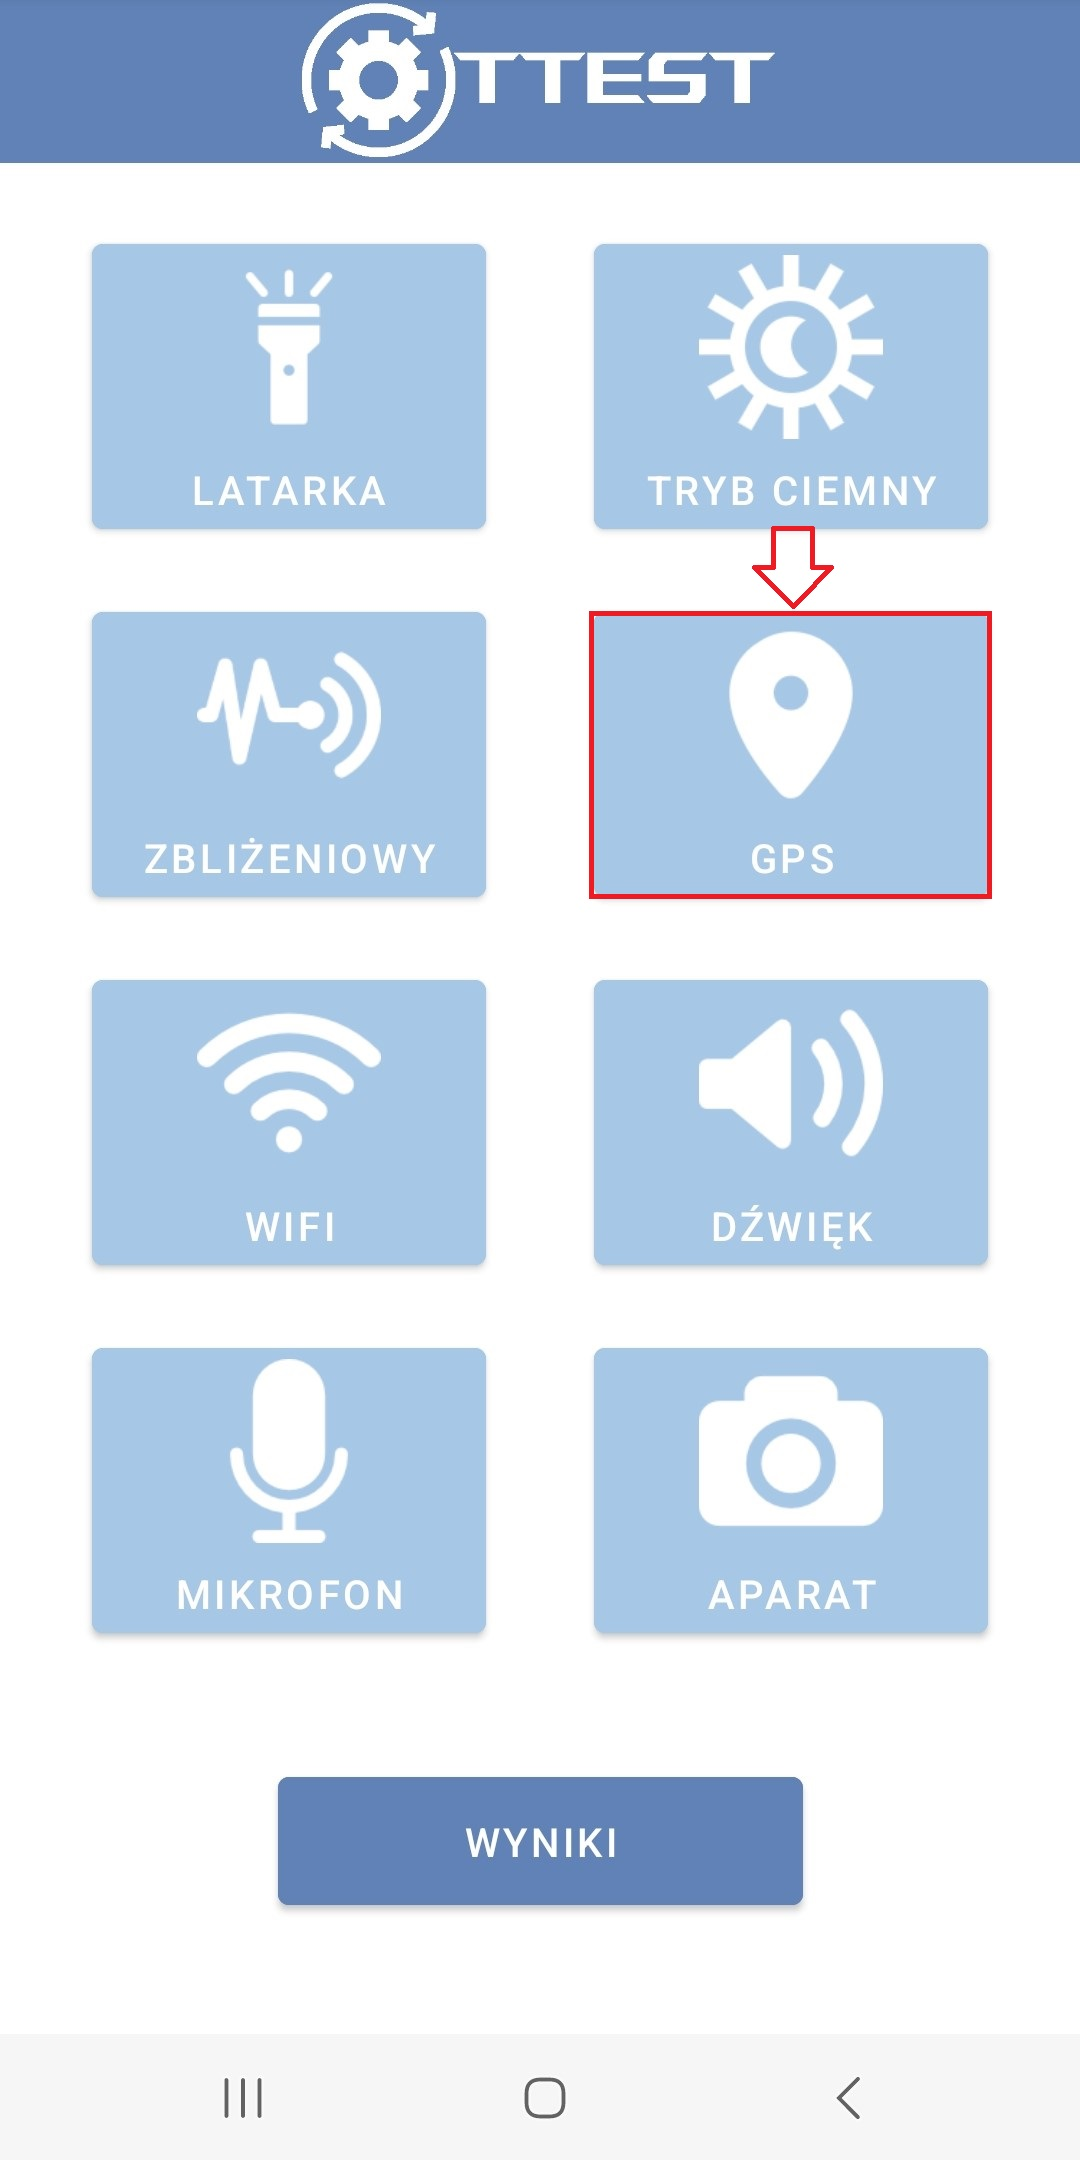
\includegraphics[angle=360, width=0.45\textwidth]{rys/punkt6/menu4}
		\caption{Wybór testu lokaliacji}
		\label{rys:menu4}
	\end{center}
\end{figure}

Po przejściu do strony z testem na środku ekranu  wyświetla nam się przycisk, którego celem jest wyszukanie naszej aktualnej lokalizacji. Rysunek \ref{rys:gps} prezentuje stronę z testem lokalizacji. \\

Gdy klikniemy na przycisk po krótkiej chwili wyświetli nam się dokładna lokalizacja - adres, kod pocztowy, miasto oraz kraj w którym obecnie się znajdujemy. Oprócz wyżej wymienionych informacji u dołu pod lokalizacją zostaje wyświetlona w formie pop-up'u szerokość i długość geograficzna.

\newpage

\begin{figure}[!hbt]
	\begin{center}
		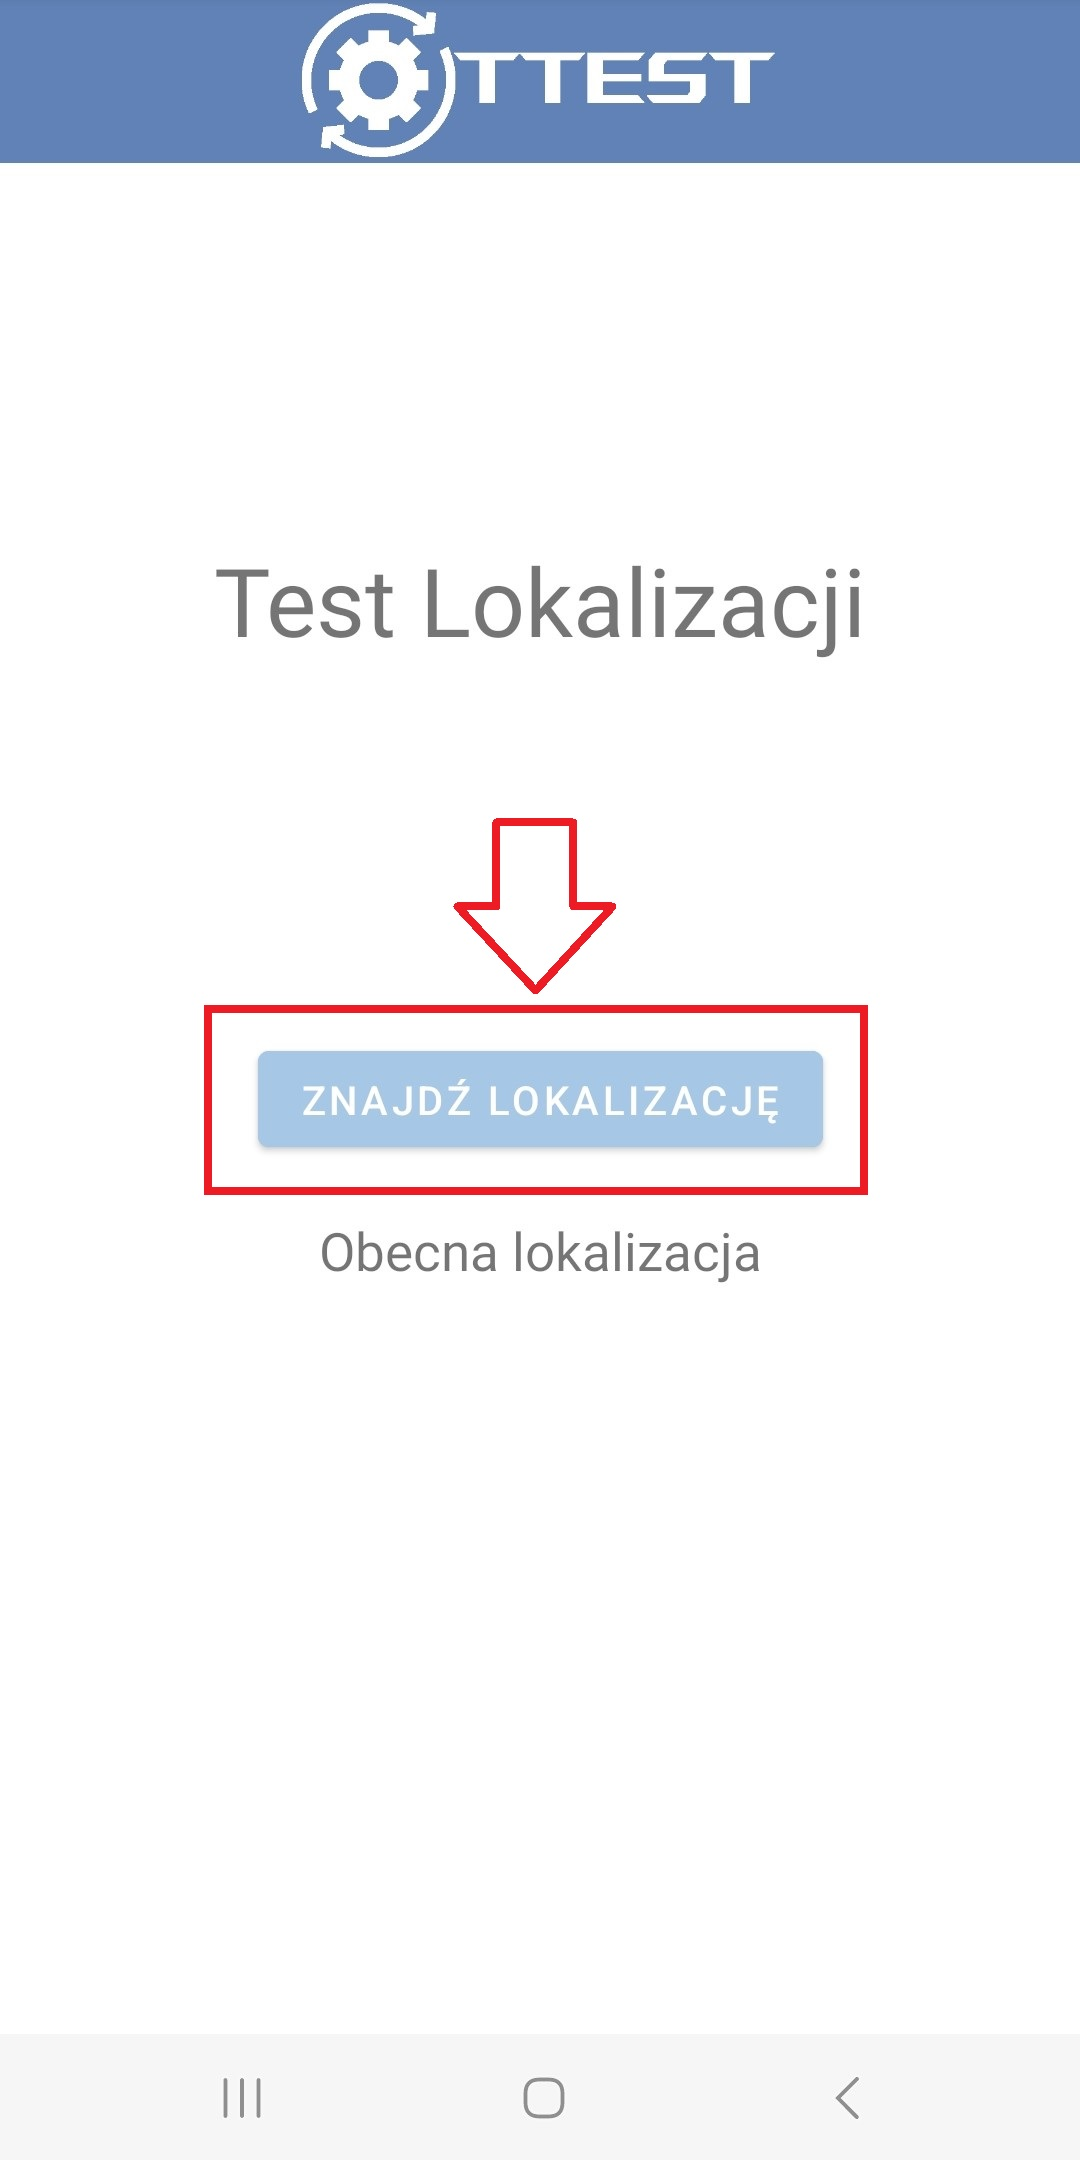
\includegraphics[angle=360, width=0.32\textwidth]{rys/punkt6/gps}
		\caption{Stona testowa lokalizacji}
		\label{rys:gps}
	\end{center}
\end{figure}

Rysunek \ref{rys:gps1} przedstawia zrzut ekranu potwierdzający pomyślny przebieg \\ testu.

\begin{figure}[!hbt]
	\begin{center}
		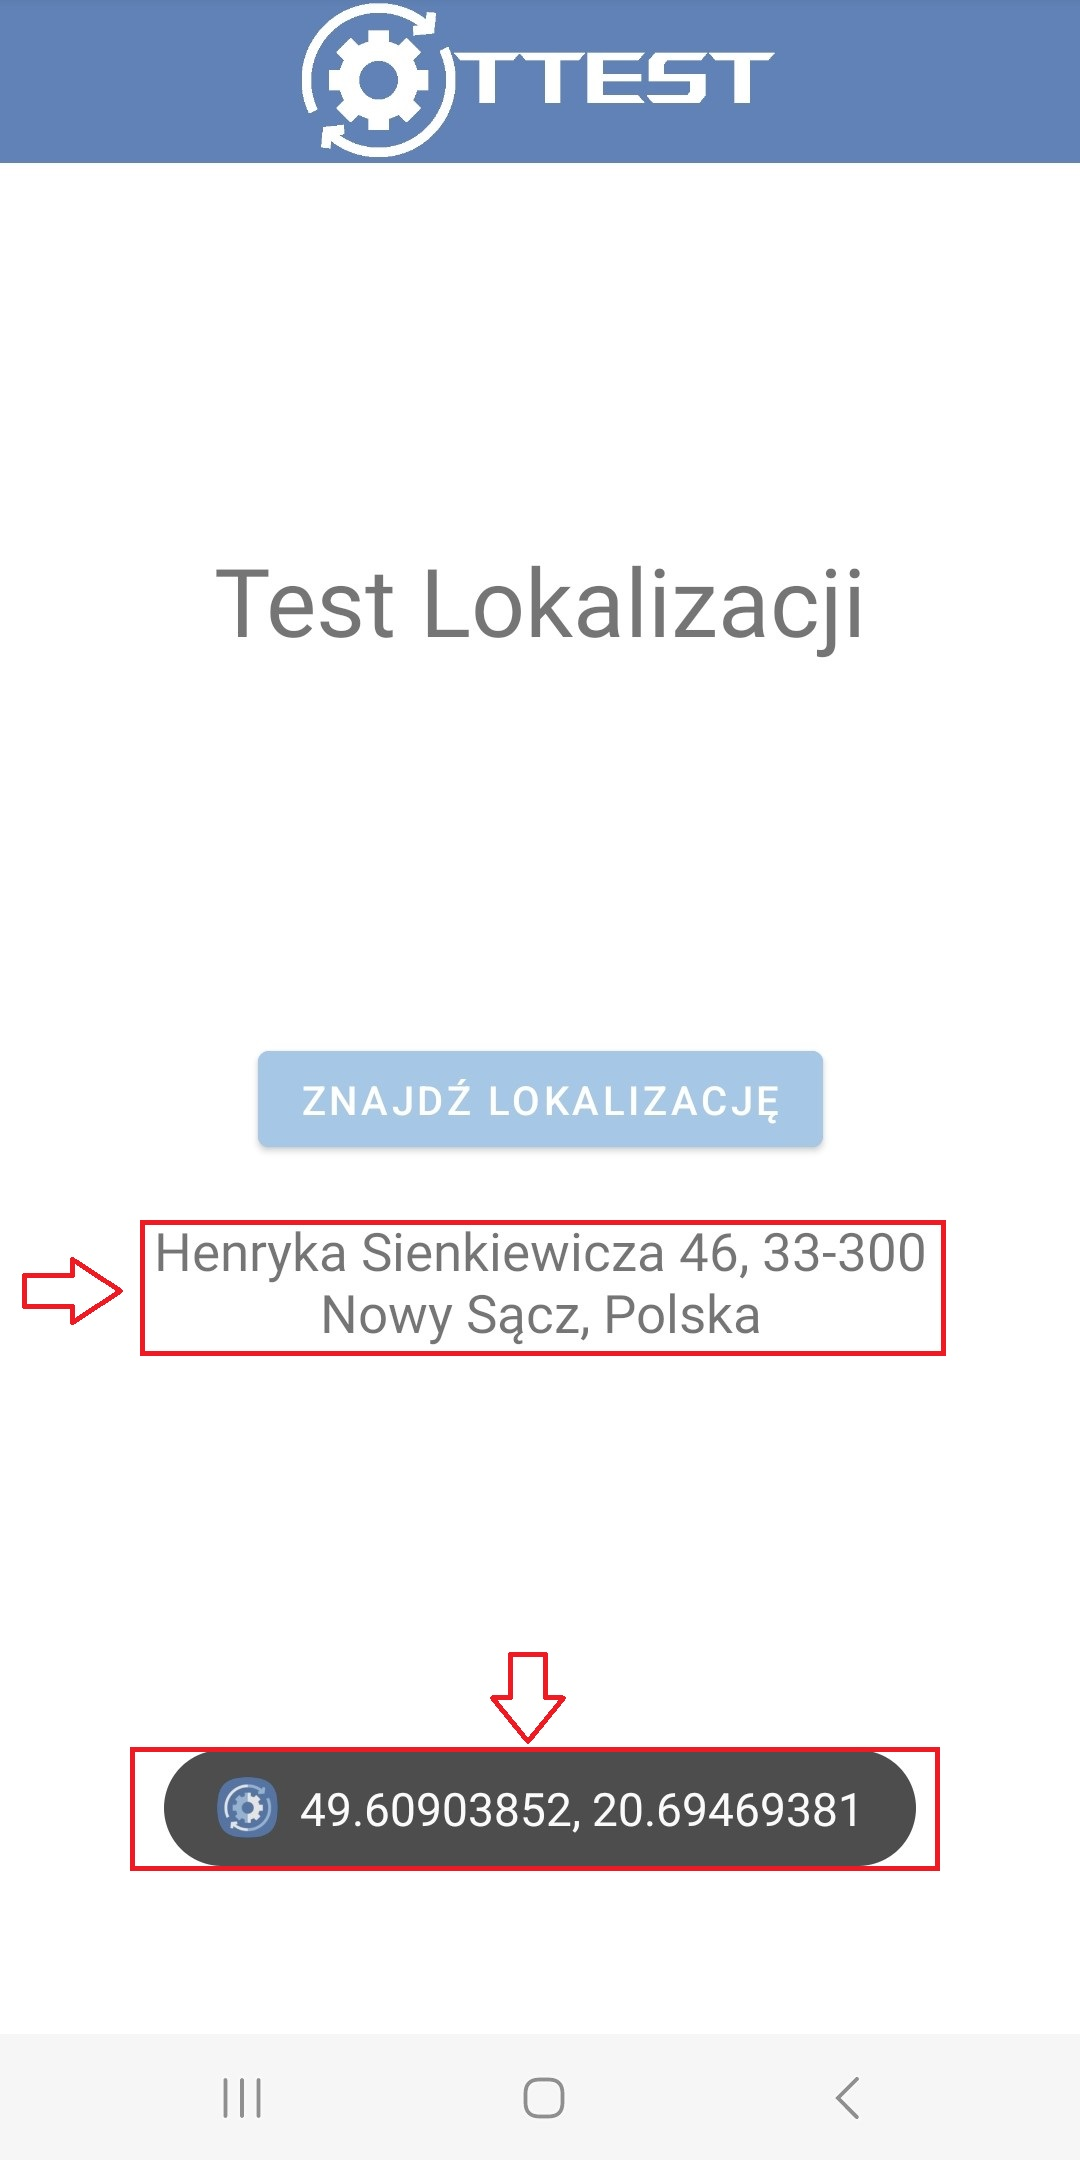
\includegraphics[angle=360, width=0.32\textwidth]{rys/punkt6/gps1}
		\caption{Działanie lokalizacji}
		\label{rys:gps1}
	\end{center}
\end{figure}

\newpage


\subsection{Test Wifi}

\hspace{0.60cm}Aby uruchomić test wifi, w menu głównego wybieramy i klikamy na ikonkę, która znajduję się tuż pod testem czujnika zbliżeniowego. Rysunek \ref{rys:wifi} ukazuję kafelek który należy wybrać aby przejść do testu wifi. 

\begin{figure}[!hbt]
	\begin{center}
		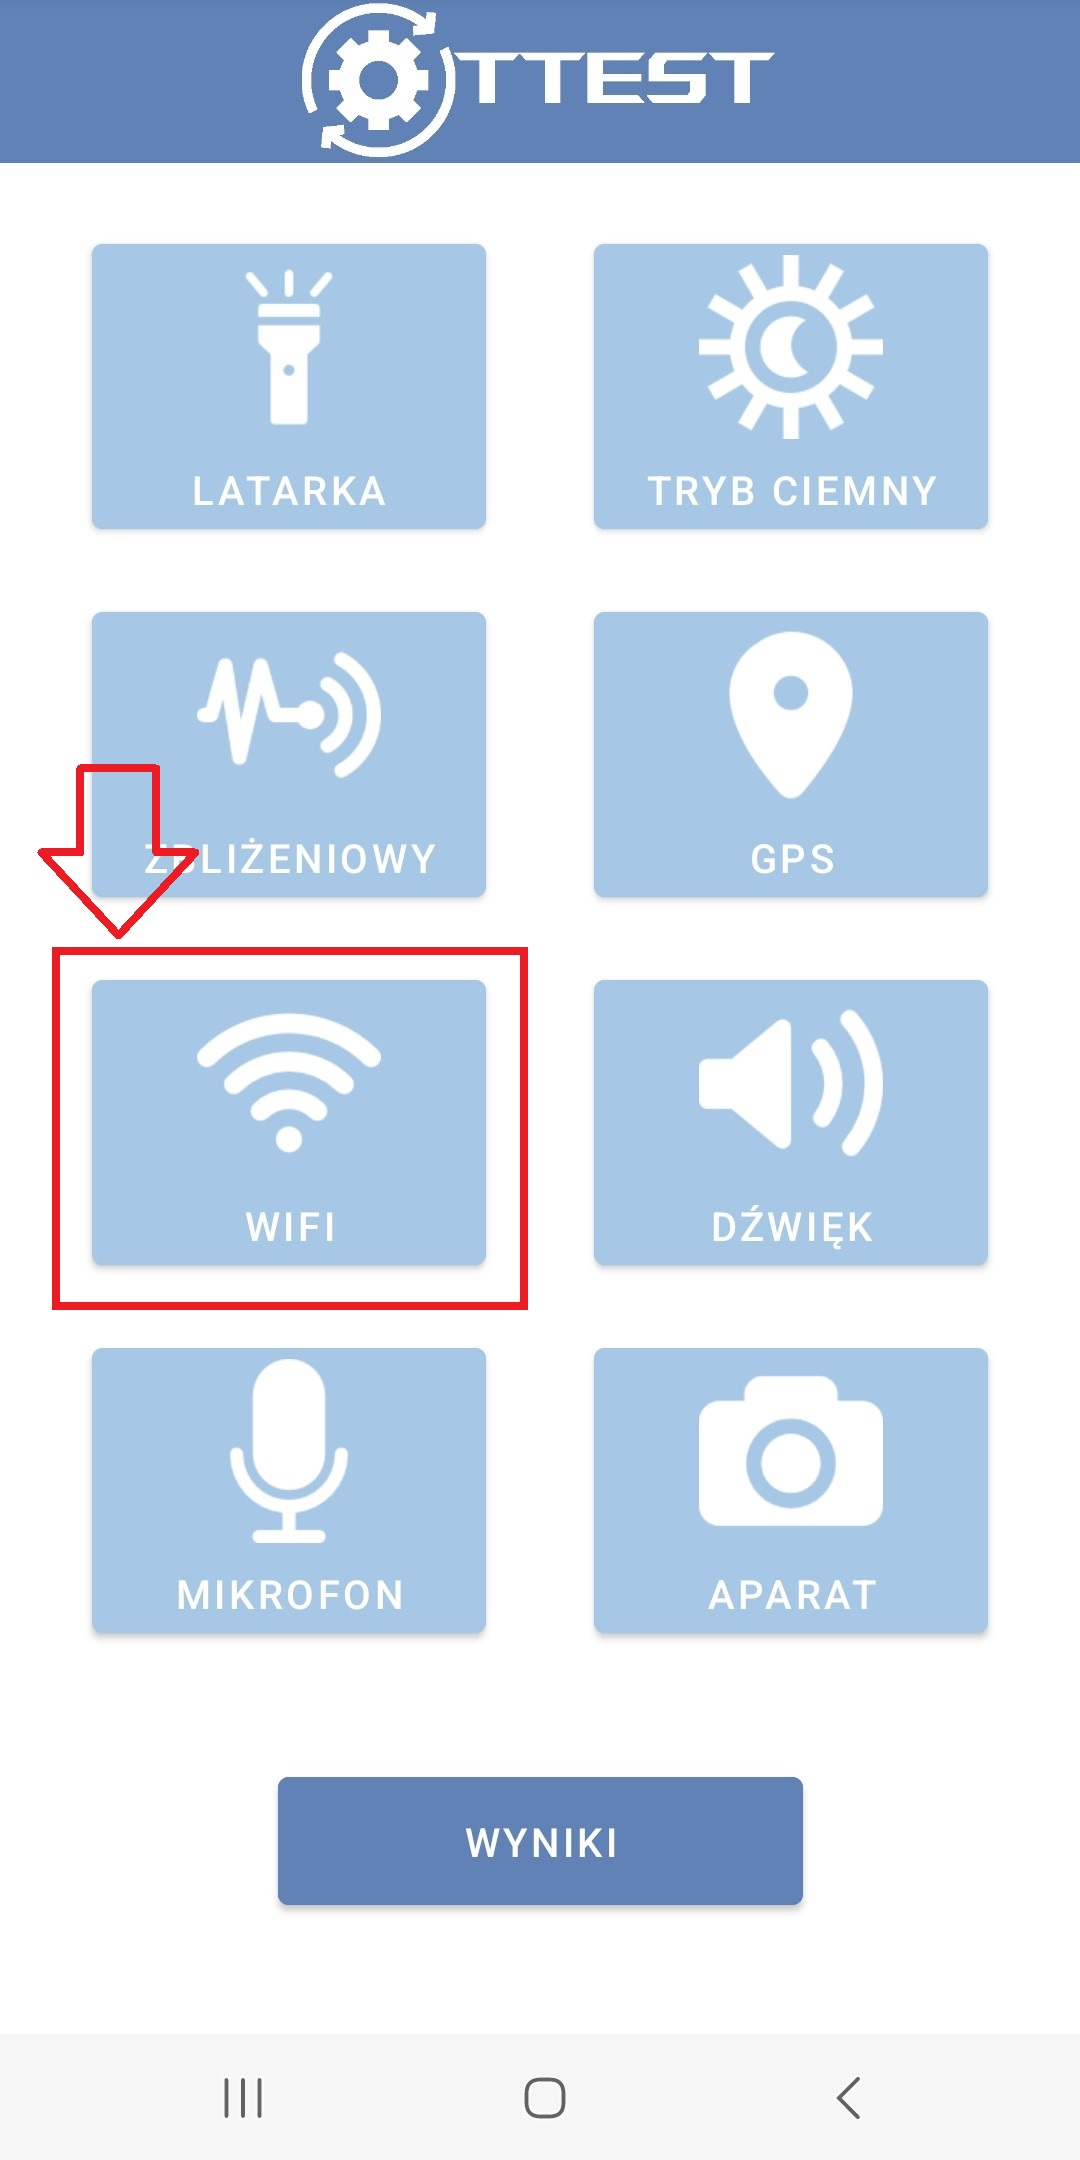
\includegraphics[angle=360, width=0.45\textwidth]{rys/punkt6/wifi}
		\caption{Wybór wifi}
		\label{rys:wifi}
	\end{center}
\end{figure}

\newpage 


Po przejściu do strony z testem wifi otrzymujemy informację aby uruchomić wifi na naszym telefonie i połączyć się z dostępną siecią. W innym przypadku nie będzie możliwe wykonanie testu oraz nie otrzymamy informacji o sieci. \\
Rysunek \ref{rys:wifi1} prezentuje stronę z testem wifi.

\begin{figure}[!hbt]
	\begin{center}
		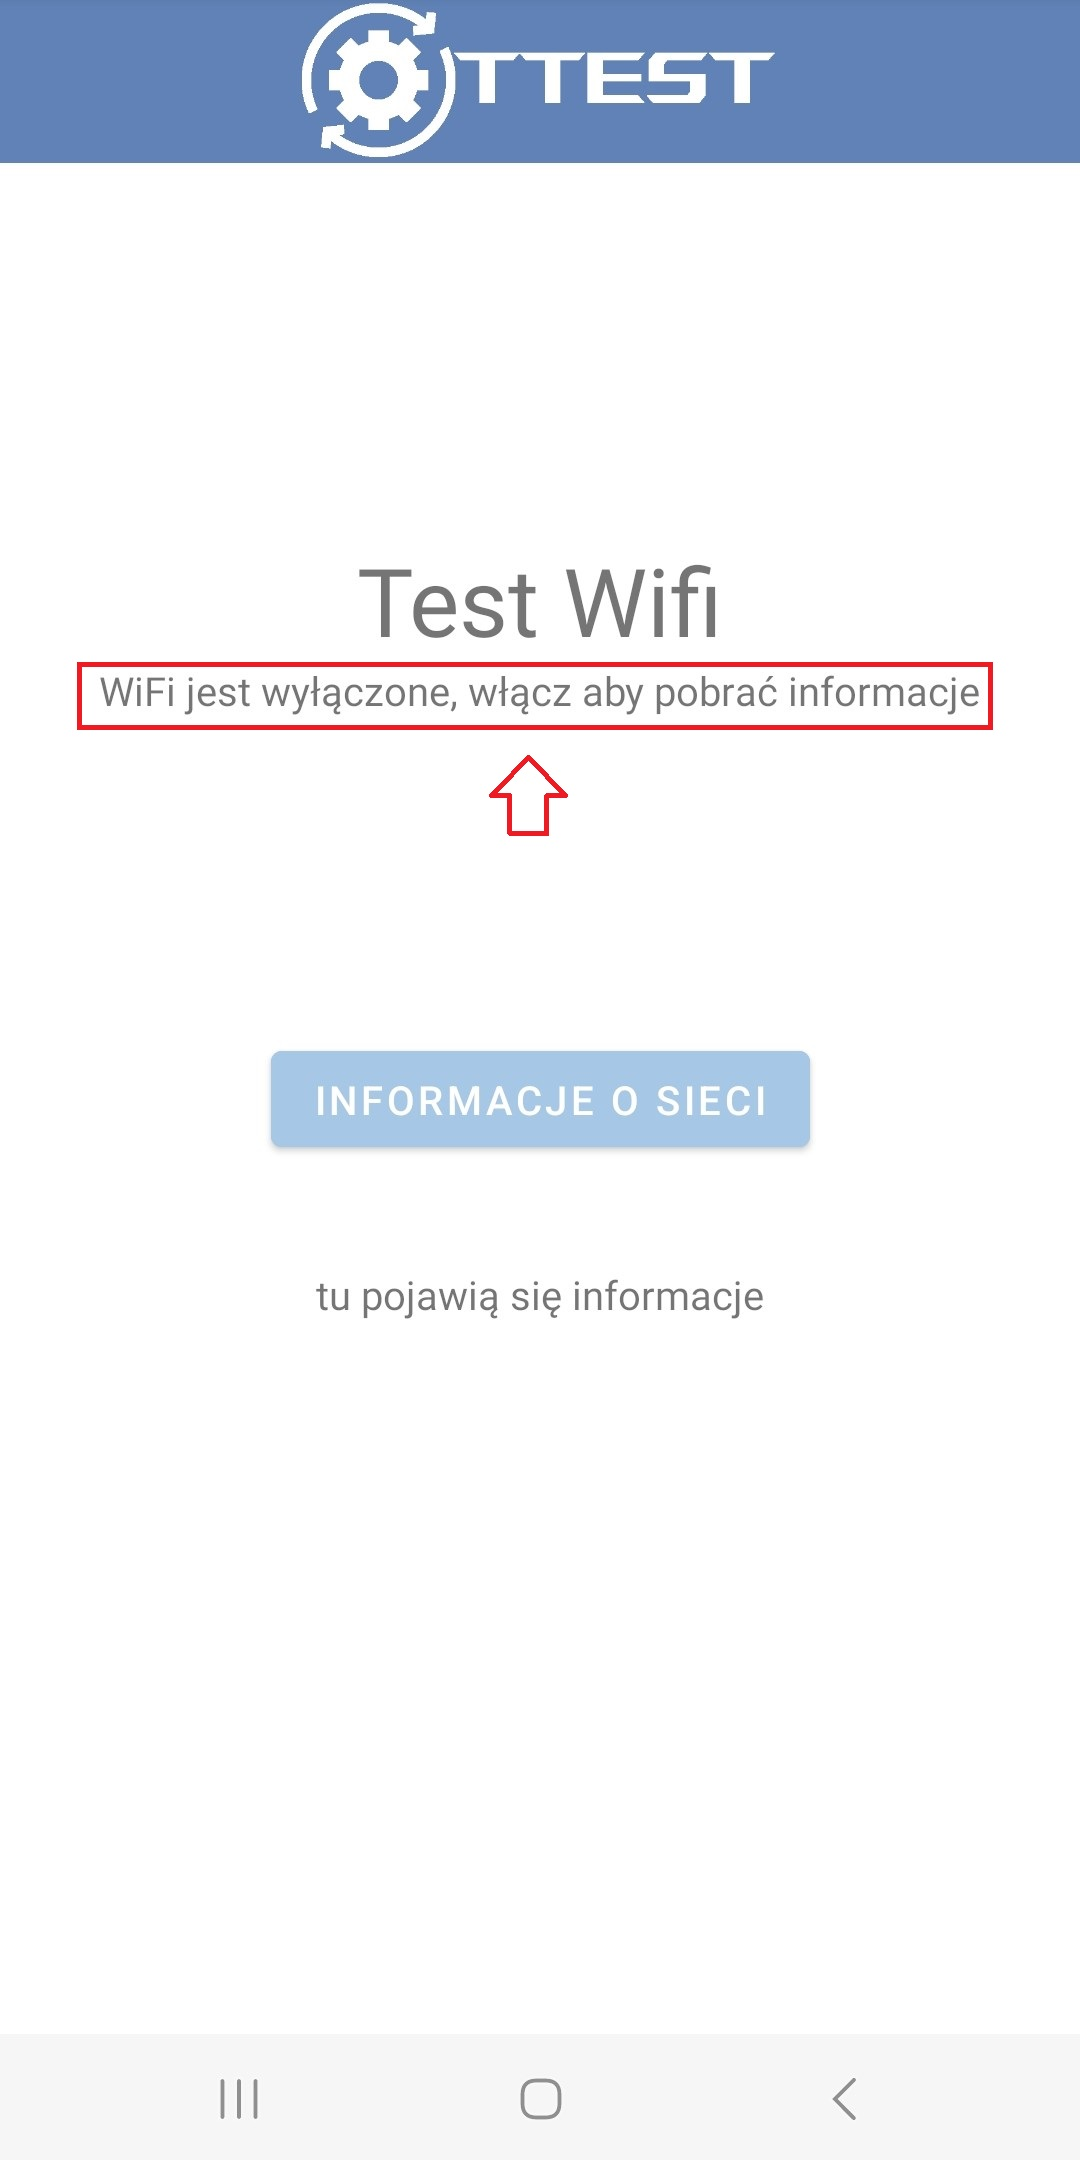
\includegraphics[angle=360, width=0.45\textwidth]{rys/punkt6/wifi1}
		\caption{Strona testowa wifi}
		\label{rys:wifi1}
	\end{center}
\end{figure}

\newpage


Po połączeniu się z siecią za pomocą wifi, otrzymujemy komunikat który mówi, że aktualnie jesteśmy połączeni z siecią i możemy pobrać dostępne informację o niej. Aby otrzymać informacje o sieci należy kliknąć na przycisk znajdujący się na środku "Informacje o sieci". \\
Rysunek \ref{rys:wifi2} prezentuje stronę z testem wifi po podłączeniu się do sieci.

\begin{figure}[!hbt]
	\begin{center}
		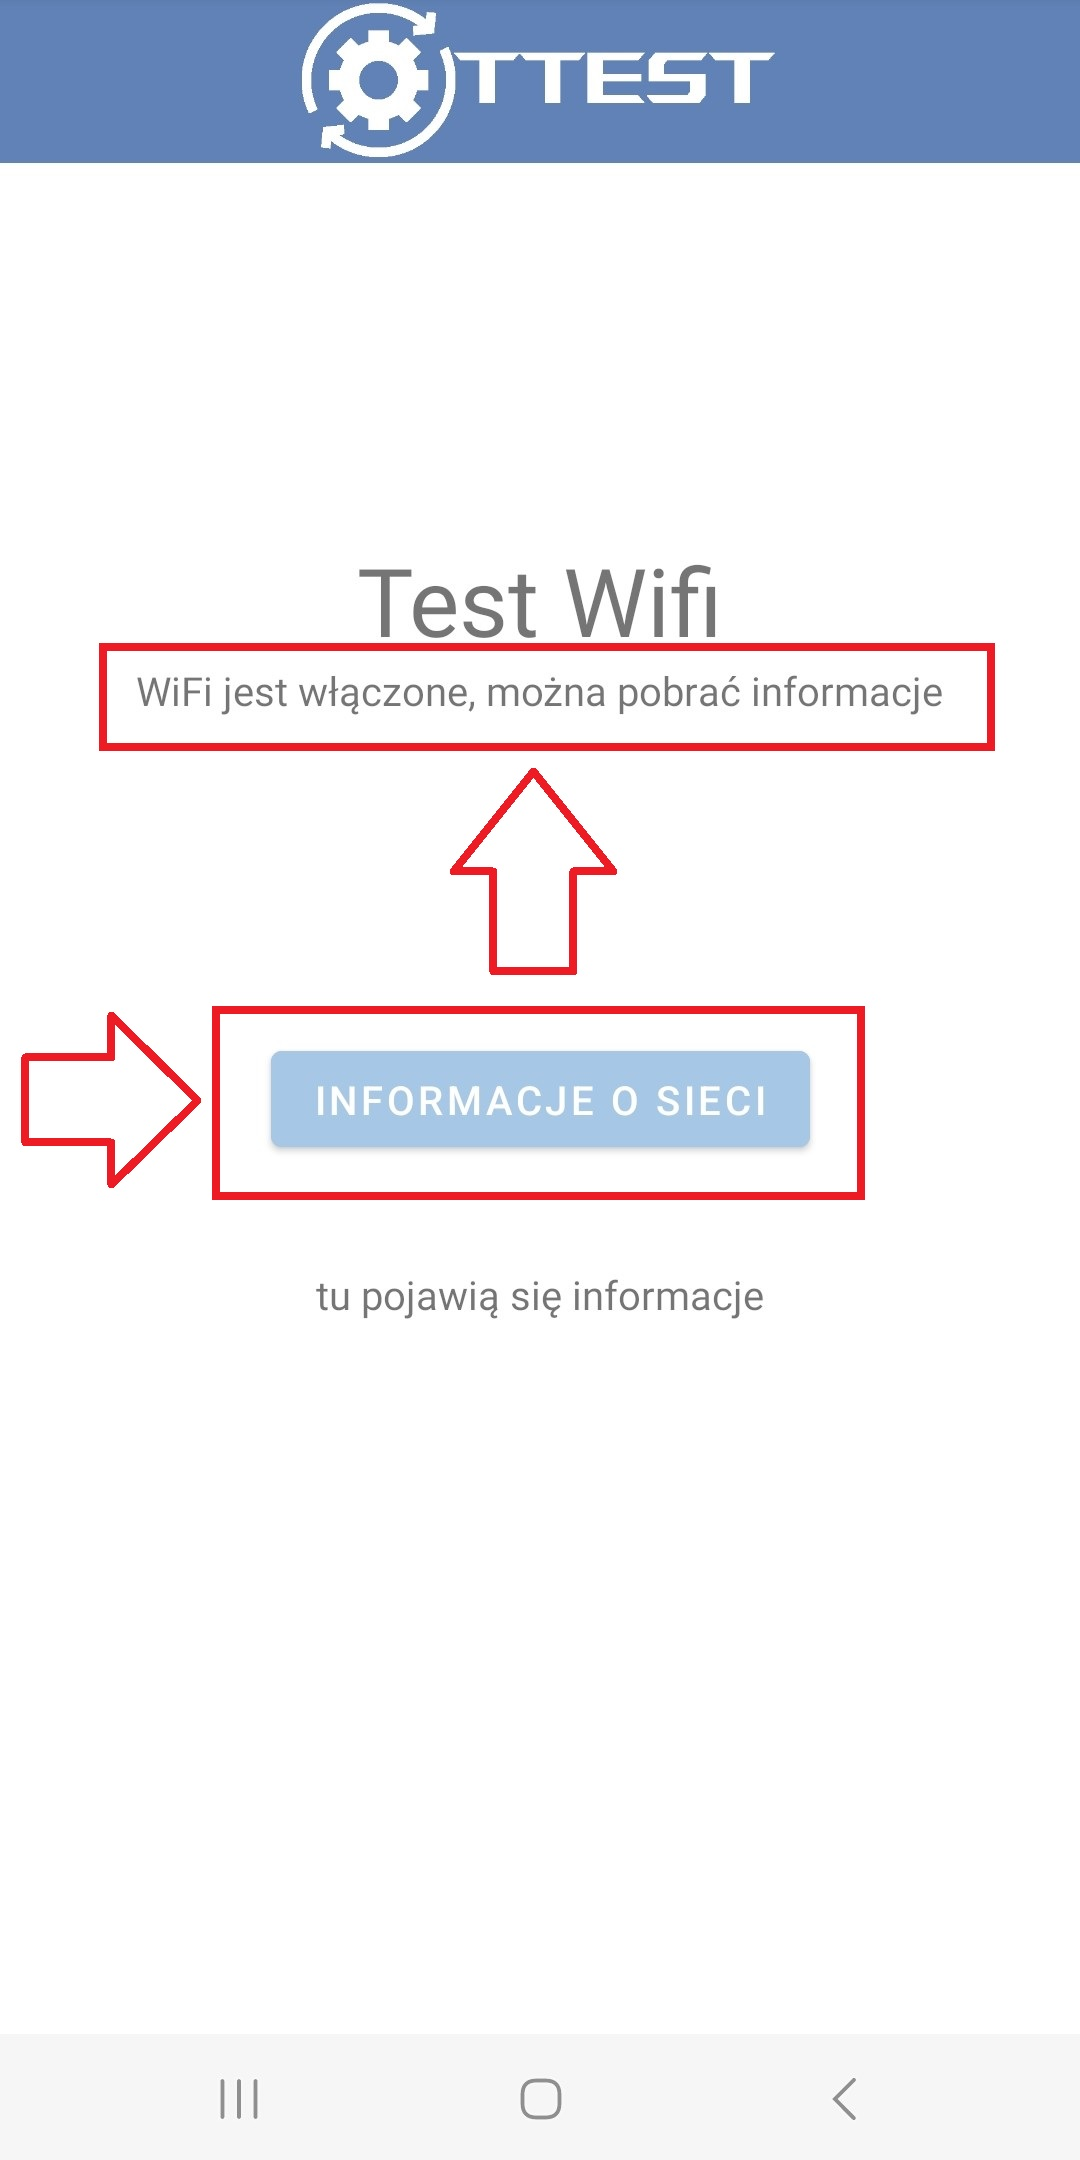
\includegraphics[angle=360, width=0.45\textwidth]{rys/punkt6/wifi2}
		\caption{Test wifi}
		\label{rys:wifi2}
	\end{center}
\end{figure}

\newpage


Po naciśnięciu na przycisk "Informacje o sieci" pojawią nam się wszystkie dostępne informacje o naszej sieci między innymi: Adres IP, Adres MAC Routera, SSID sieci do której jesteśmy podłączeni oraz wskaźnik mocy. \\
Rysunek \ref{rys:wifi3} przedstawia zrzut ekranu potwierdzający pomyślny przebieg testu.

\begin{figure}[!hbt]
	\begin{center}
		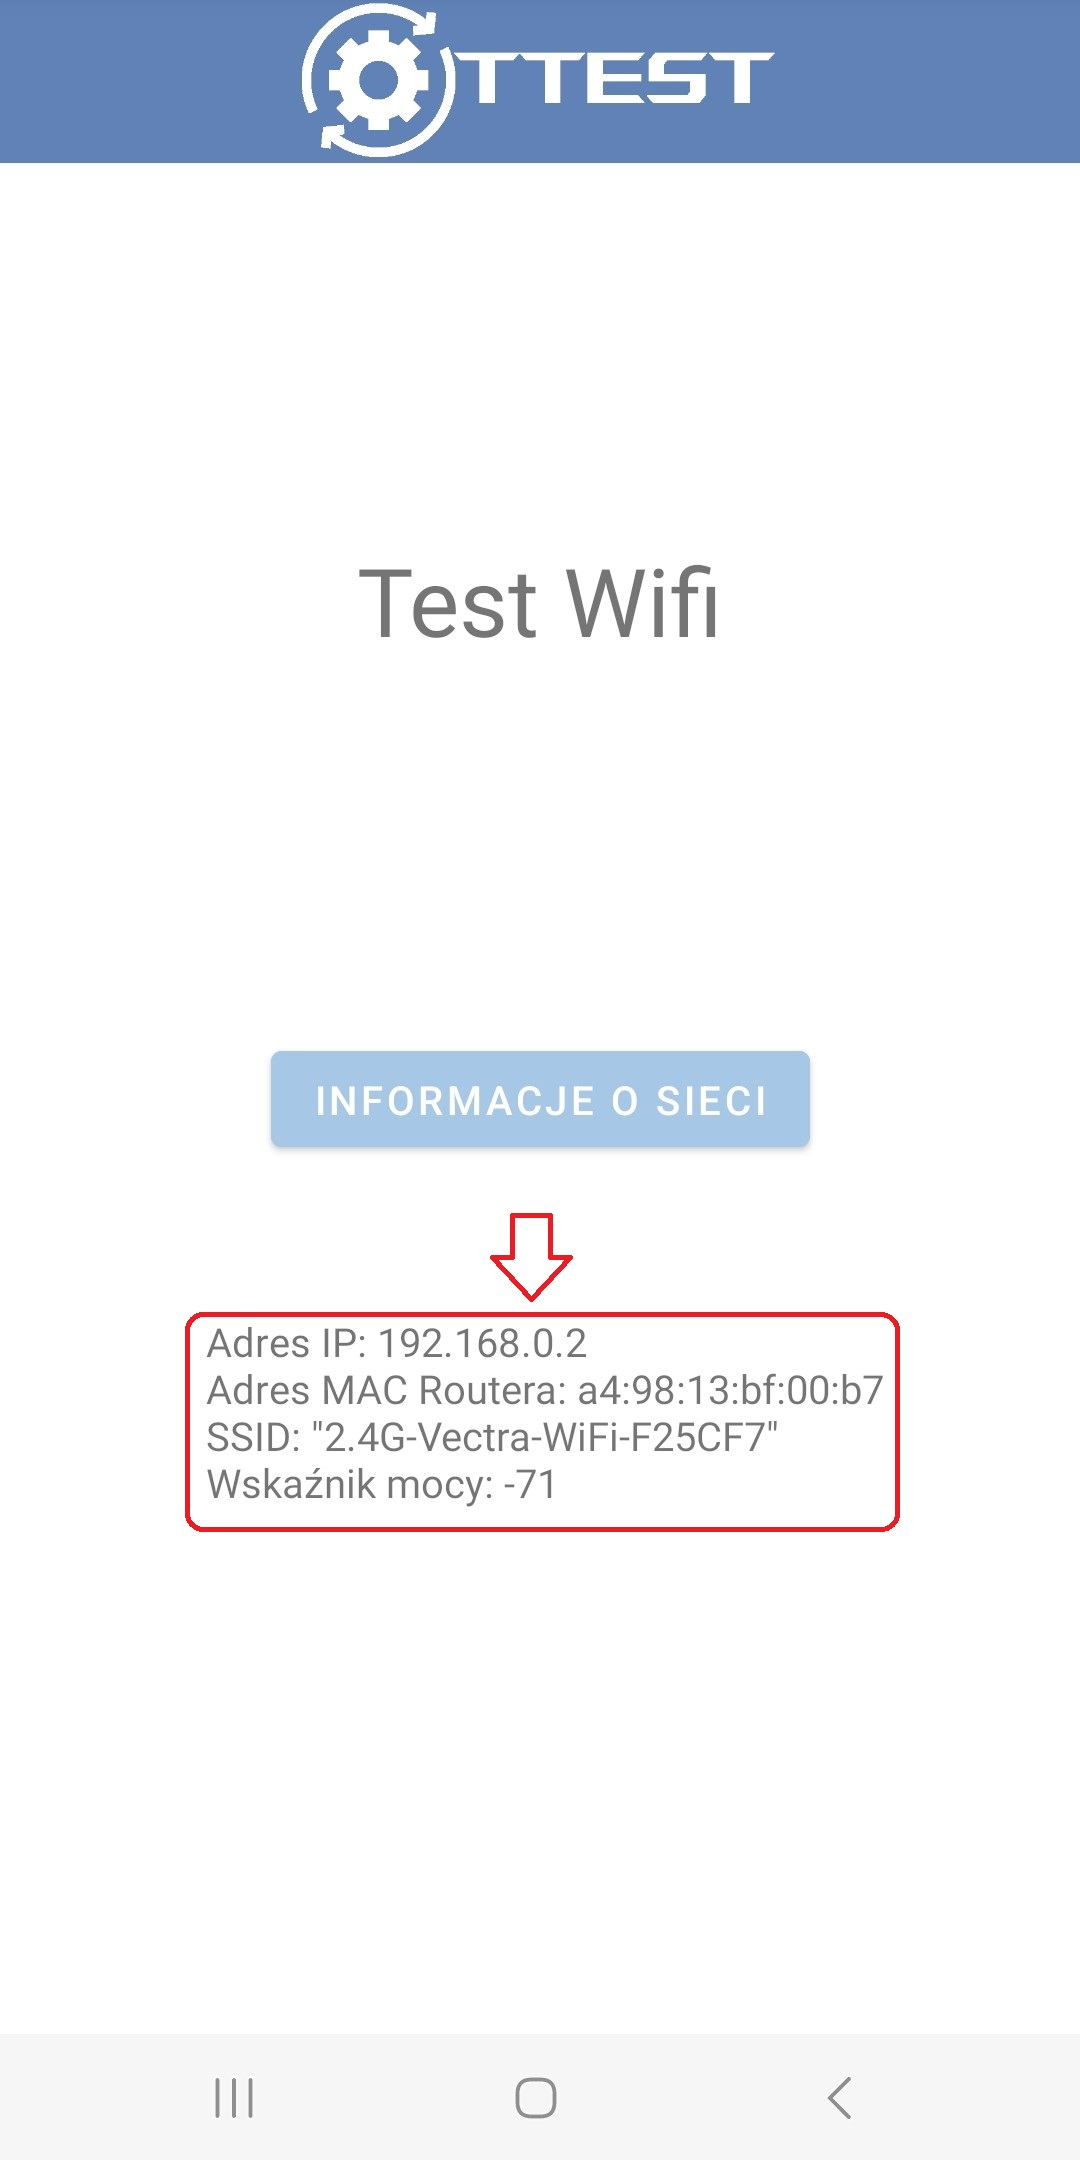
\includegraphics[angle=360, width=0.45\textwidth]{rys/punkt6/wifi3}
		\caption{Działanie wifi}
		\label{rys:wifi3}
	\end{center}
\end{figure}

\newpage


\subsection{Test dźwięku}

\hspace{0.60cm}Aby przejść do testu dźwięku należy kliknąć przycisk znajdujący się po prawej stronie tuż pod testem lokalizacji. Rysunek \ref{rys:menu5} przedstawia kafelek który należy wybrać aby przejść do testu dźwięku.

\begin{figure}[!hbt]
	\begin{center}
		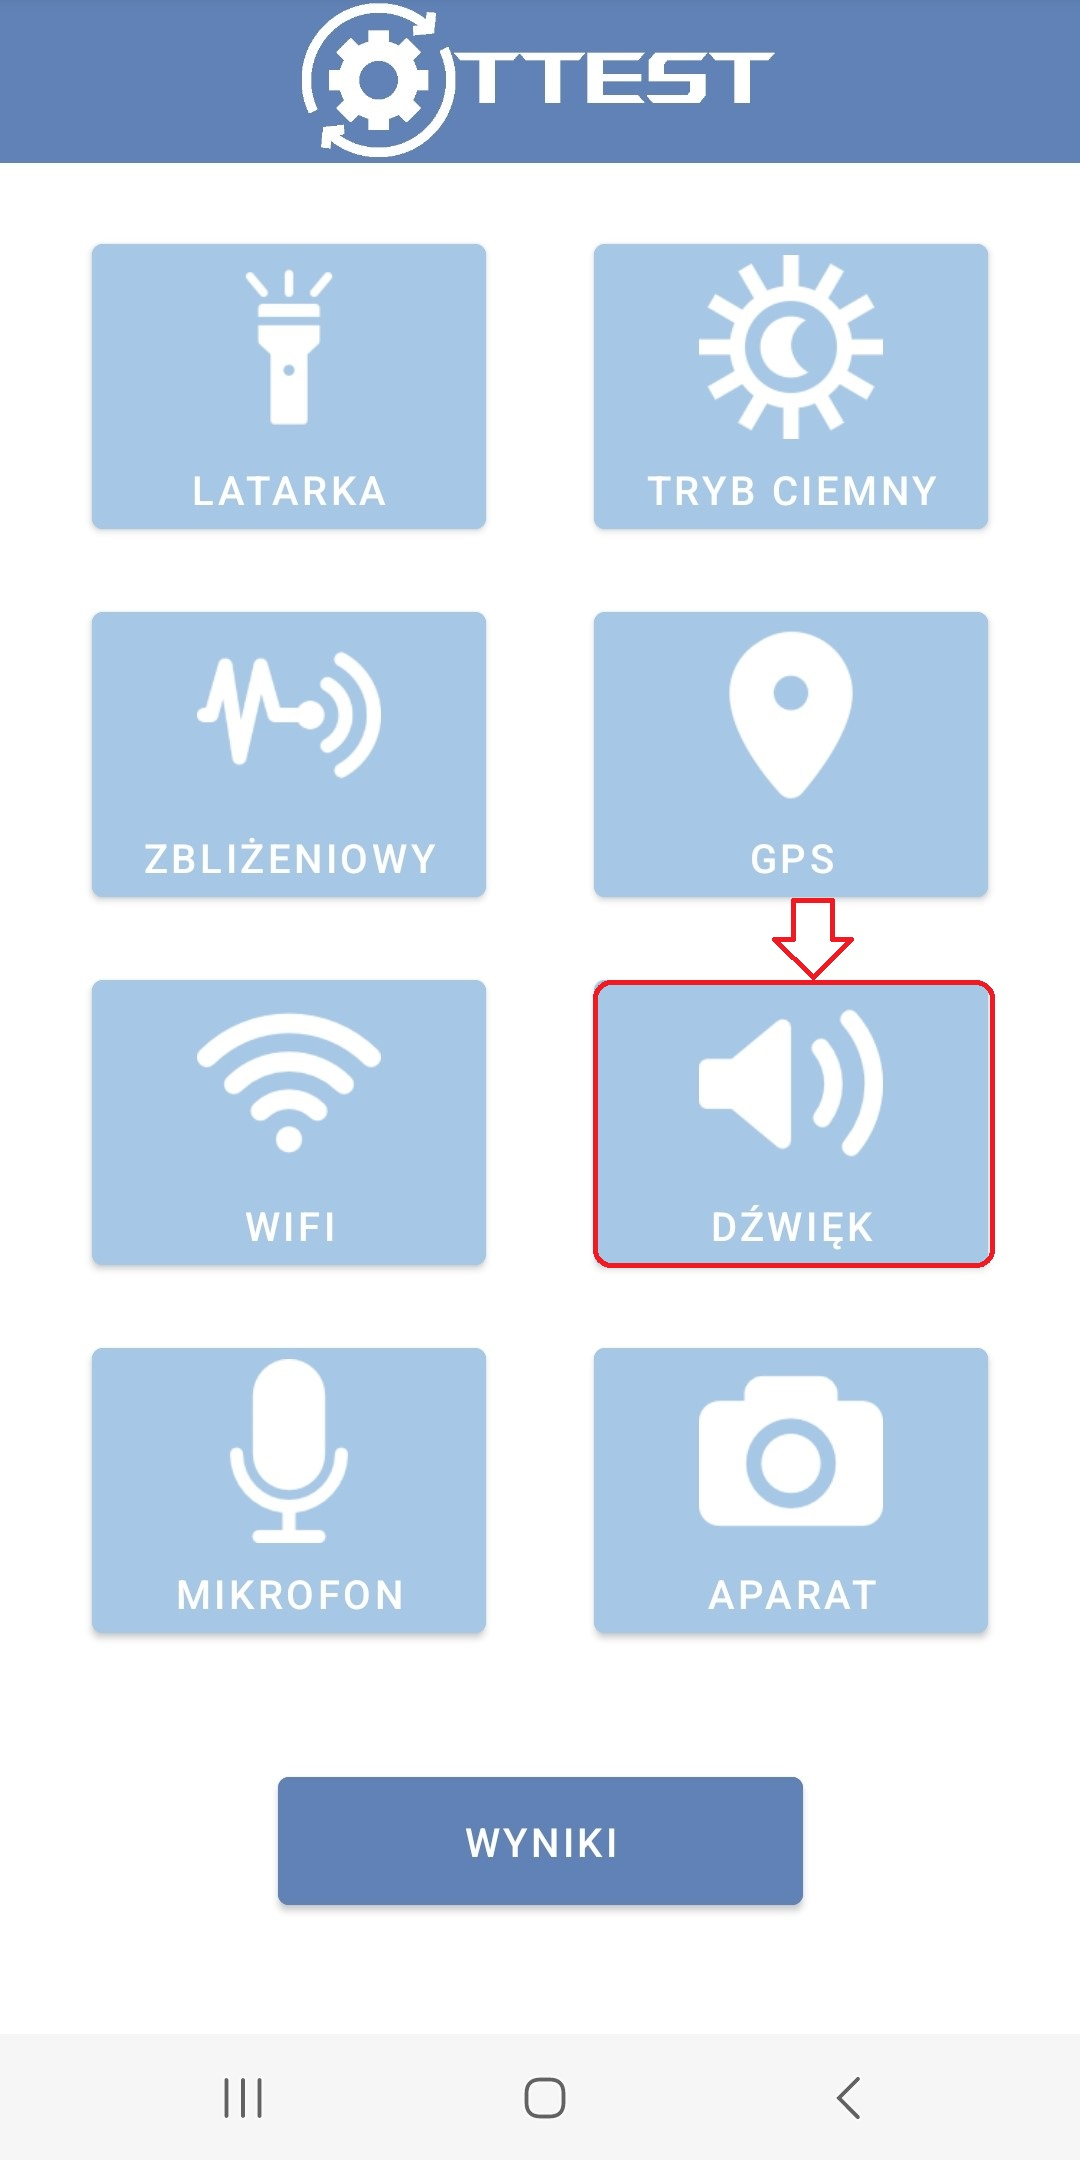
\includegraphics[angle=360, width=0.45\textwidth]{rys/punkt6/menu5}
		\caption{Wybór testu dźwięku}
		\label{rys:menu5}
	\end{center}
\end{figure}

Po przekierowaniu na stronę z testem dostrzegamy że na środku znajduję się przycisk z napisem - "Naciśnij". Rysunek \ref{rys:dźwięk} prezentuję przycisk uruchamiający test dźwięku.

Gdy naciśniemy przycisk z głośników telefonu usłyszymy dźwięk ćwierkających ptaków. Co więcej pod przyciskiem wyświetli nam się komunikat, który informuję nas o tym, że nagranie jest odtwarzane. 

\newpage

\begin{figure}[!hbt]
	\begin{center}
		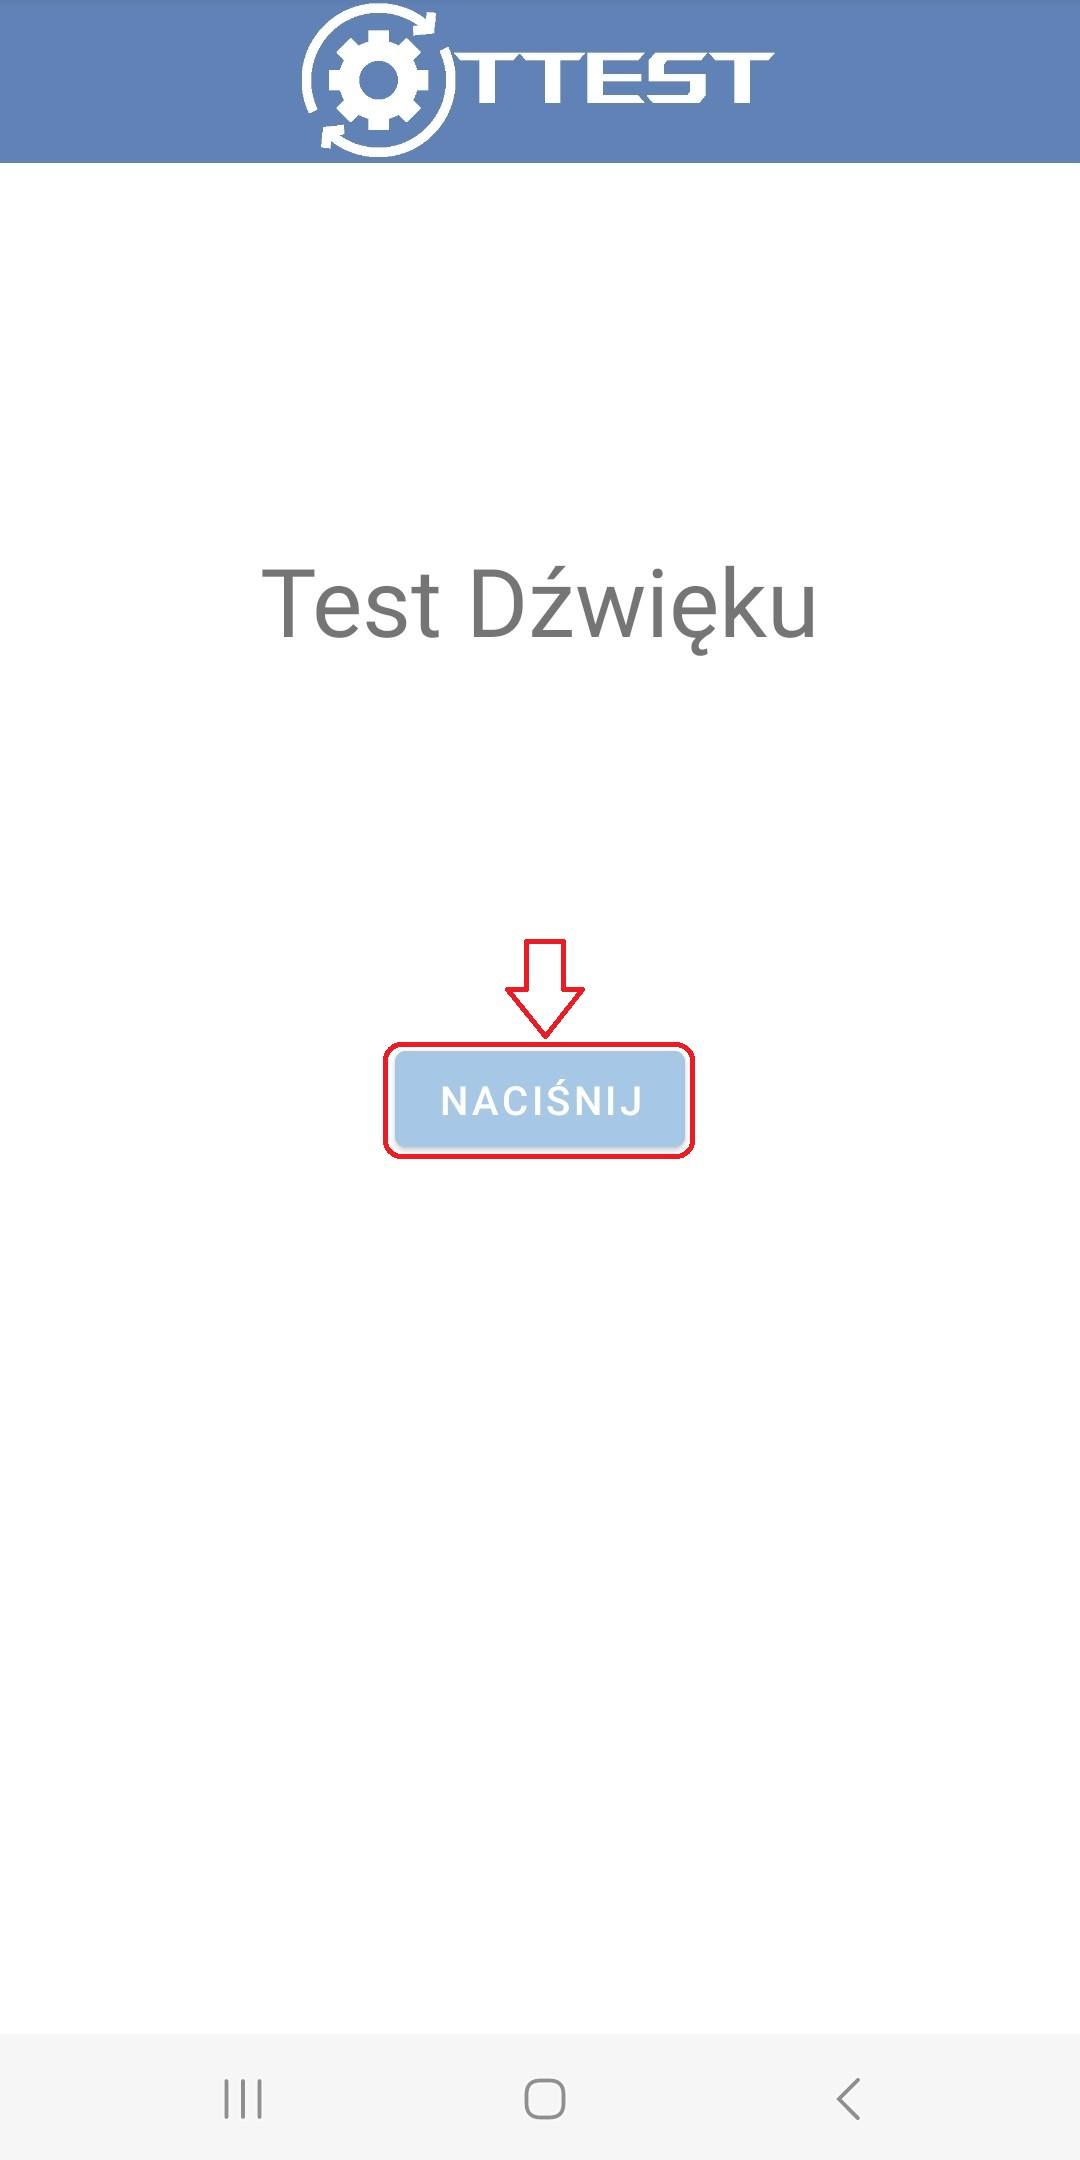
\includegraphics[angle=360, width=0.31\textwidth]{rys/punkt6/dźwięk}
		\caption{Strona testowa dźwięku}
		\label{rys:dźwięk}
	\end{center}
\end{figure}

Rysunek \ref{rys:dźwięk2} przedstawia zrzut ekranu potwierdzający pomyślny przebieg testu.

\begin{figure}[!hbt]
	\begin{center}
		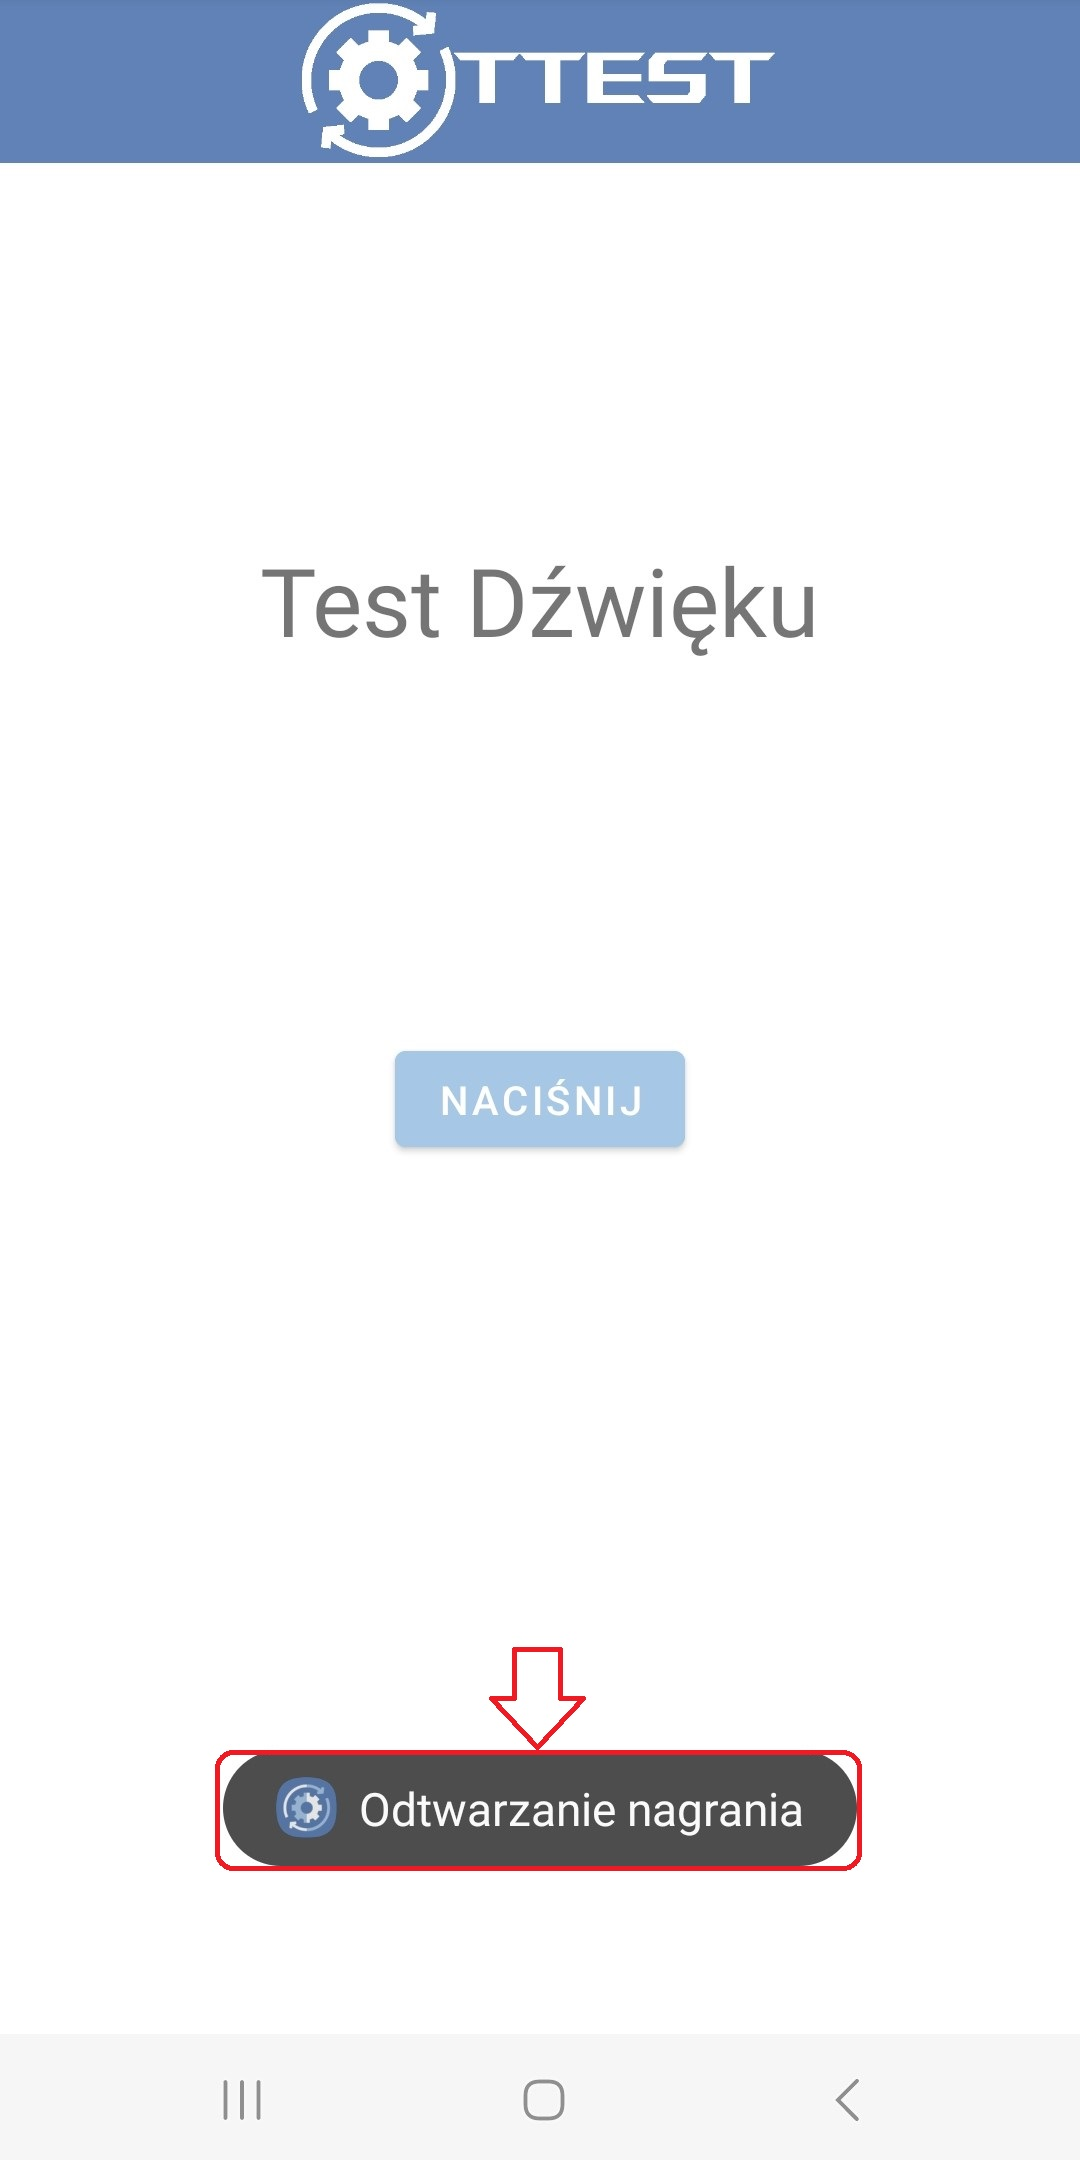
\includegraphics[angle=360, width=0.31\textwidth]{rys/punkt6/dźwięk2}
		\caption{Test dźwięku}
		\label{rys:dźwięk2}
	\end{center}
\end{figure}

\newpage


\subsection{Test mikrofonu}

\hspace{0.60cm}Aby przejść do testu mikrofonu należy kliknąć przycisk znajdujący się po lewej stronie tuż pod testem wifi. Rysunek \ref{rys:menu6} przedstawia kafelek który należy wybrać aby przejść do testu mikrofonu.

\begin{figure}[!hbt]
	\begin{center}
		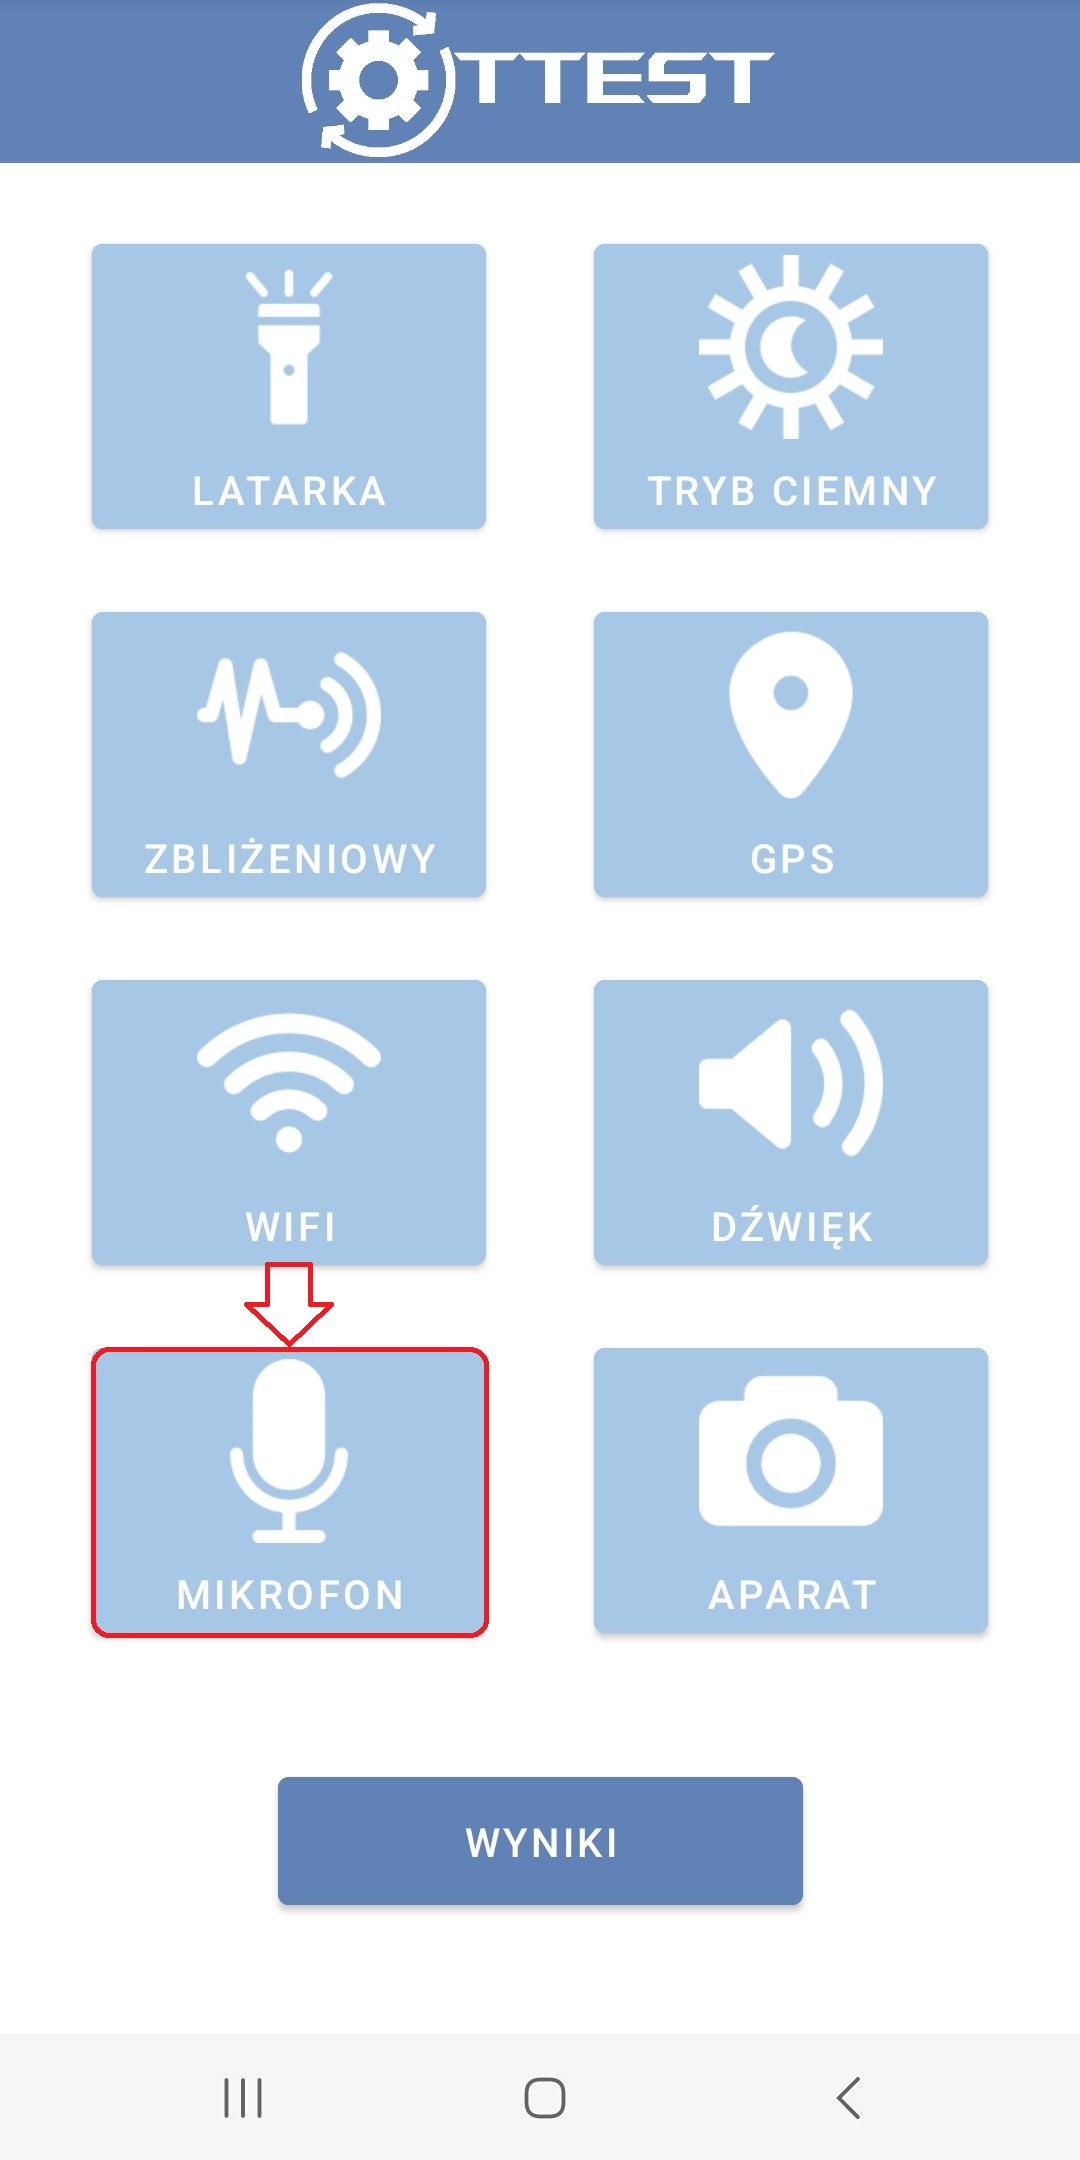
\includegraphics[angle=360, width=0.45\textwidth]{rys/punkt6/menu6}
		\caption{Wybór testu mikrofonu}
		\label{rys:menu6}
	\end{center}
\end{figure}

Po przekierowaniu na stronę z testem dostrzegamy że na środku znajduję się trzry przyciski kolejno: Start, Stop oraz Play. 

\newpage


Przycisk z napisem - "Start" rozpoczyna test oraz nagrywa wszystko to co mówimy. Ponadto u dołu ekranu pojawia się komunikat, który informuję nas o rozpoczęciu nagrywania. Rysunek \ref{rys:mikrofon1} prezentuję przycisk startu w teście mikrofonu.

\begin{figure}[!hbt]
	\begin{center}
		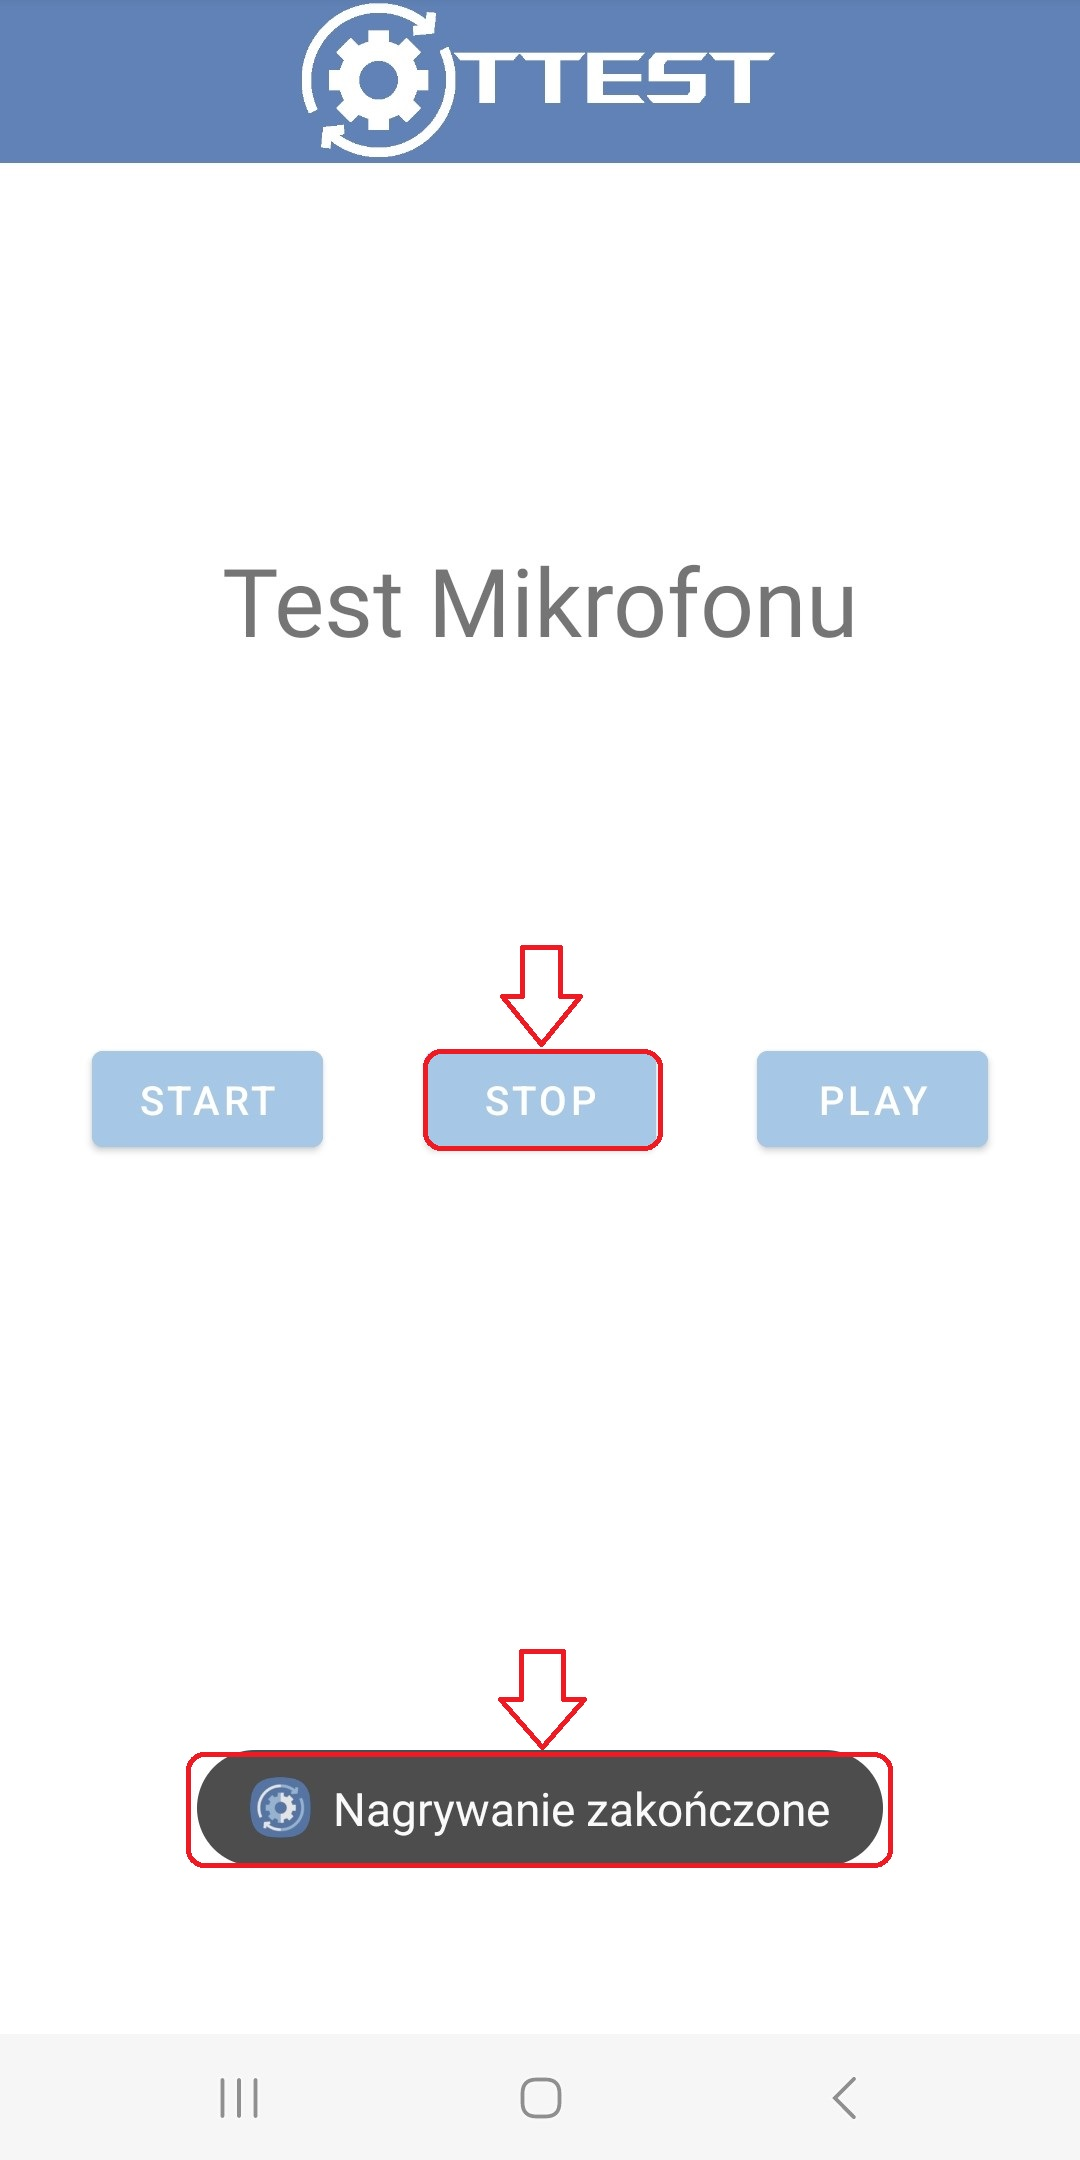
\includegraphics[angle=360, width=0.45\textwidth]{rys/punkt6/mikrofon1}
		\caption{Działanie przycisku Start - Mikrofon}
		\label{rys:mikrofon1}
	\end{center}
\end{figure}

\newpage


Aby zatrzymać nagrywanie wystarczy przycisnąć drugi przycisk - "Stop". \\ Podobnie jak w przypadku przycisku "Start", u dołu ekranu pojawi się informacja o tym, że nagrywanie zostało zakończone. Rysunek \ref{rys:mikrofon2} prezentuję przycisk stopu w teście mikrofonu.

\begin{figure}[!hbt]
	\begin{center}
		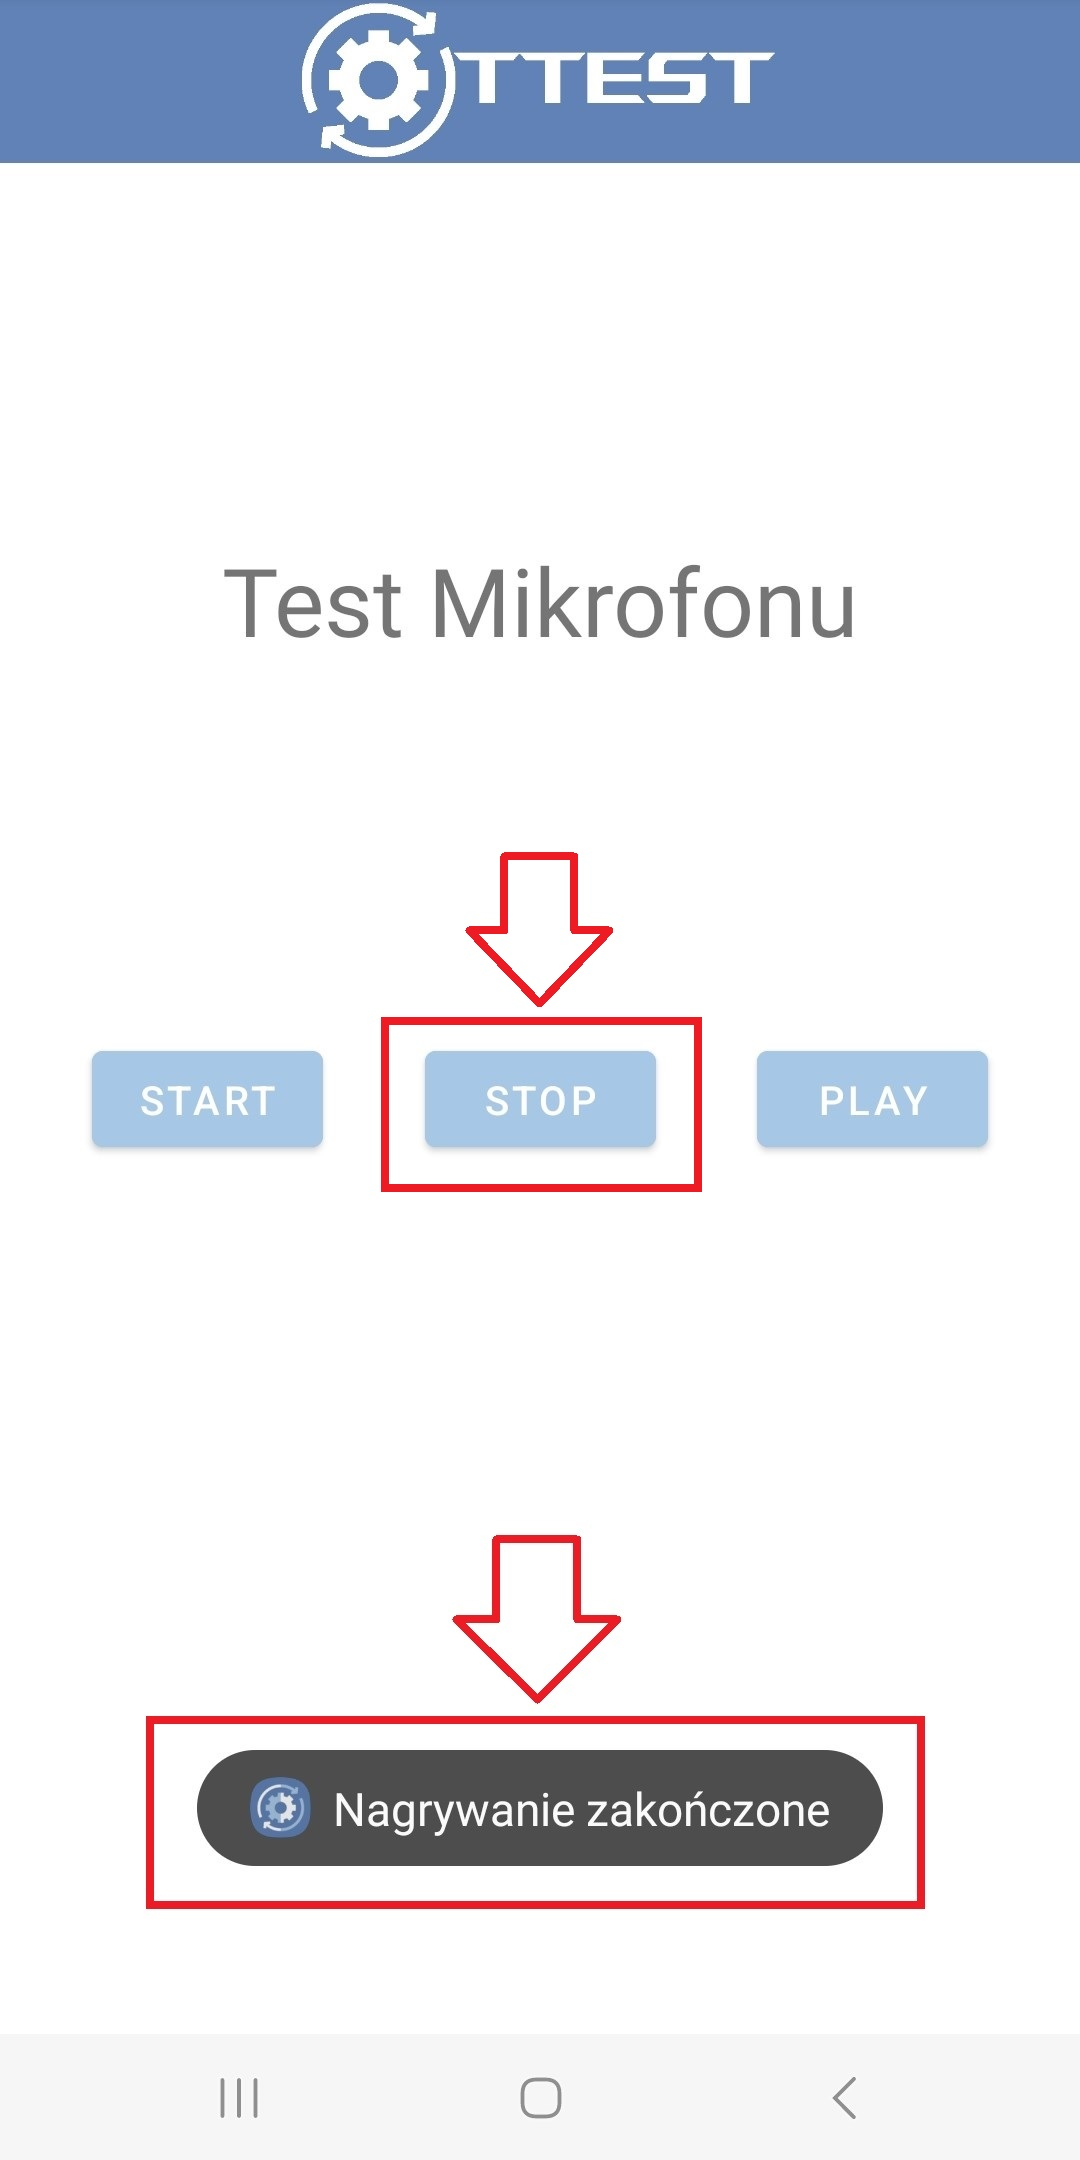
\includegraphics[angle=360, width=0.45\textwidth]{rys/punkt6/mikrofon2}
		\caption{Działanie przycisku Stop - Mikrofon}
		\label{rys:mikrofon2}
	\end{center}
\end{figure}

\newpage


Ostatni z przycisków - "Play" pozwala na odtworzenie nagranego wcześniej nagrania. Pod przyciskami zarówno jak przy przycisku start jak i stop, pojawia się informacja o tym, że nagranie jest odtwarzane. Rysunek \ref{rys:mikrofon3} prezentuję przycisk play w teście mikrofonu.

\begin{figure}[!hbt]
	\begin{center}
		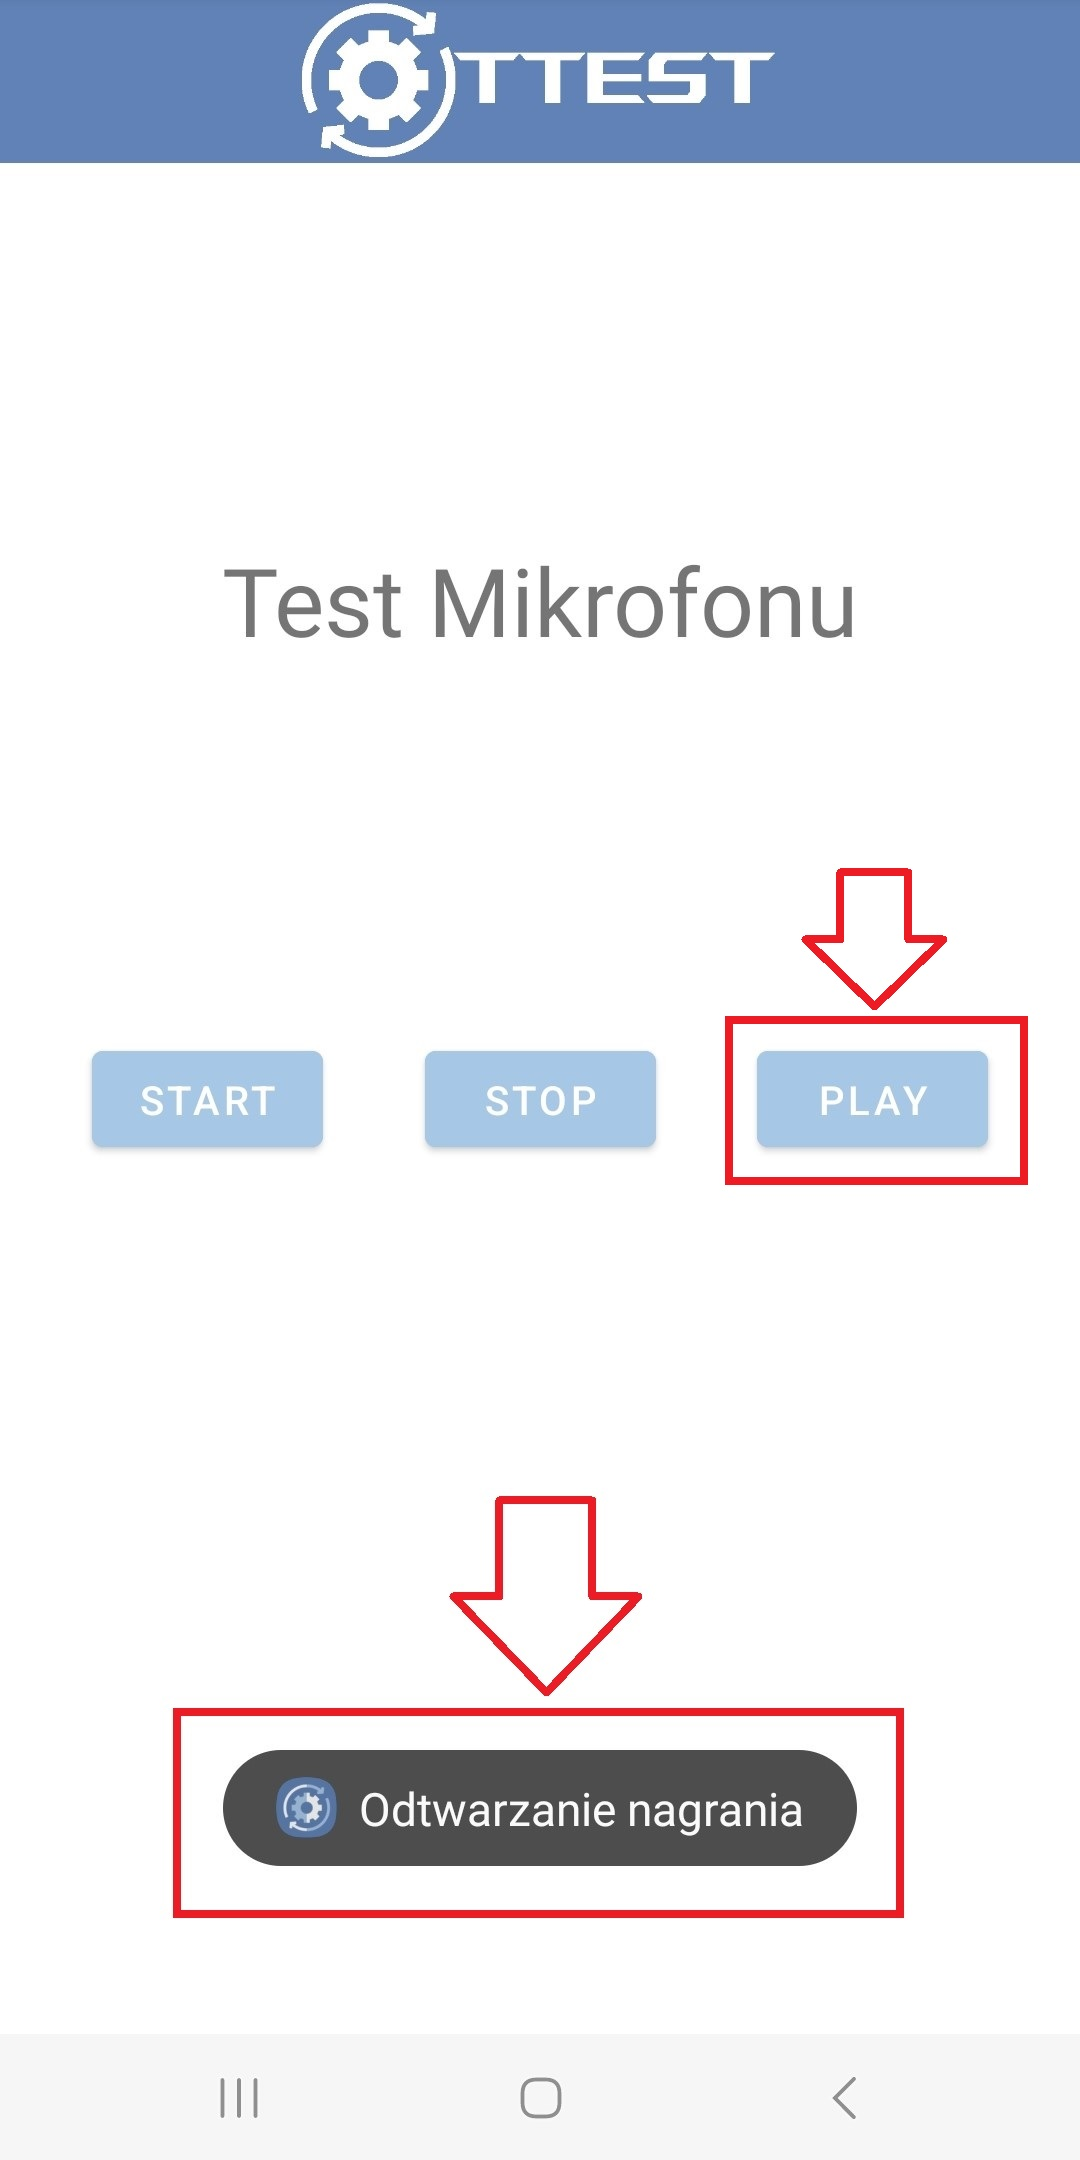
\includegraphics[angle=360, width=0.45\textwidth]{rys/punkt6/mikrofon3}
		\caption{Działanie przycisku Play - Mikrofon}
		\label{rys:mikrofon3}
	\end{center}
\end{figure}

\newpage


\subsection{Test aparatu}

\hspace{0.60cm}Aby przejść do testu aparatu należy w menu głównym wybrać i kliknąć przycisk znajdujący się po prawej stronie tuż pod testem dźwięku. Rysunek \ref{rys:menu7} przedstawia kafelek który należy wybrać aby przejść do testu aparatu.

\begin{figure}[!hbt]
	\begin{center}
		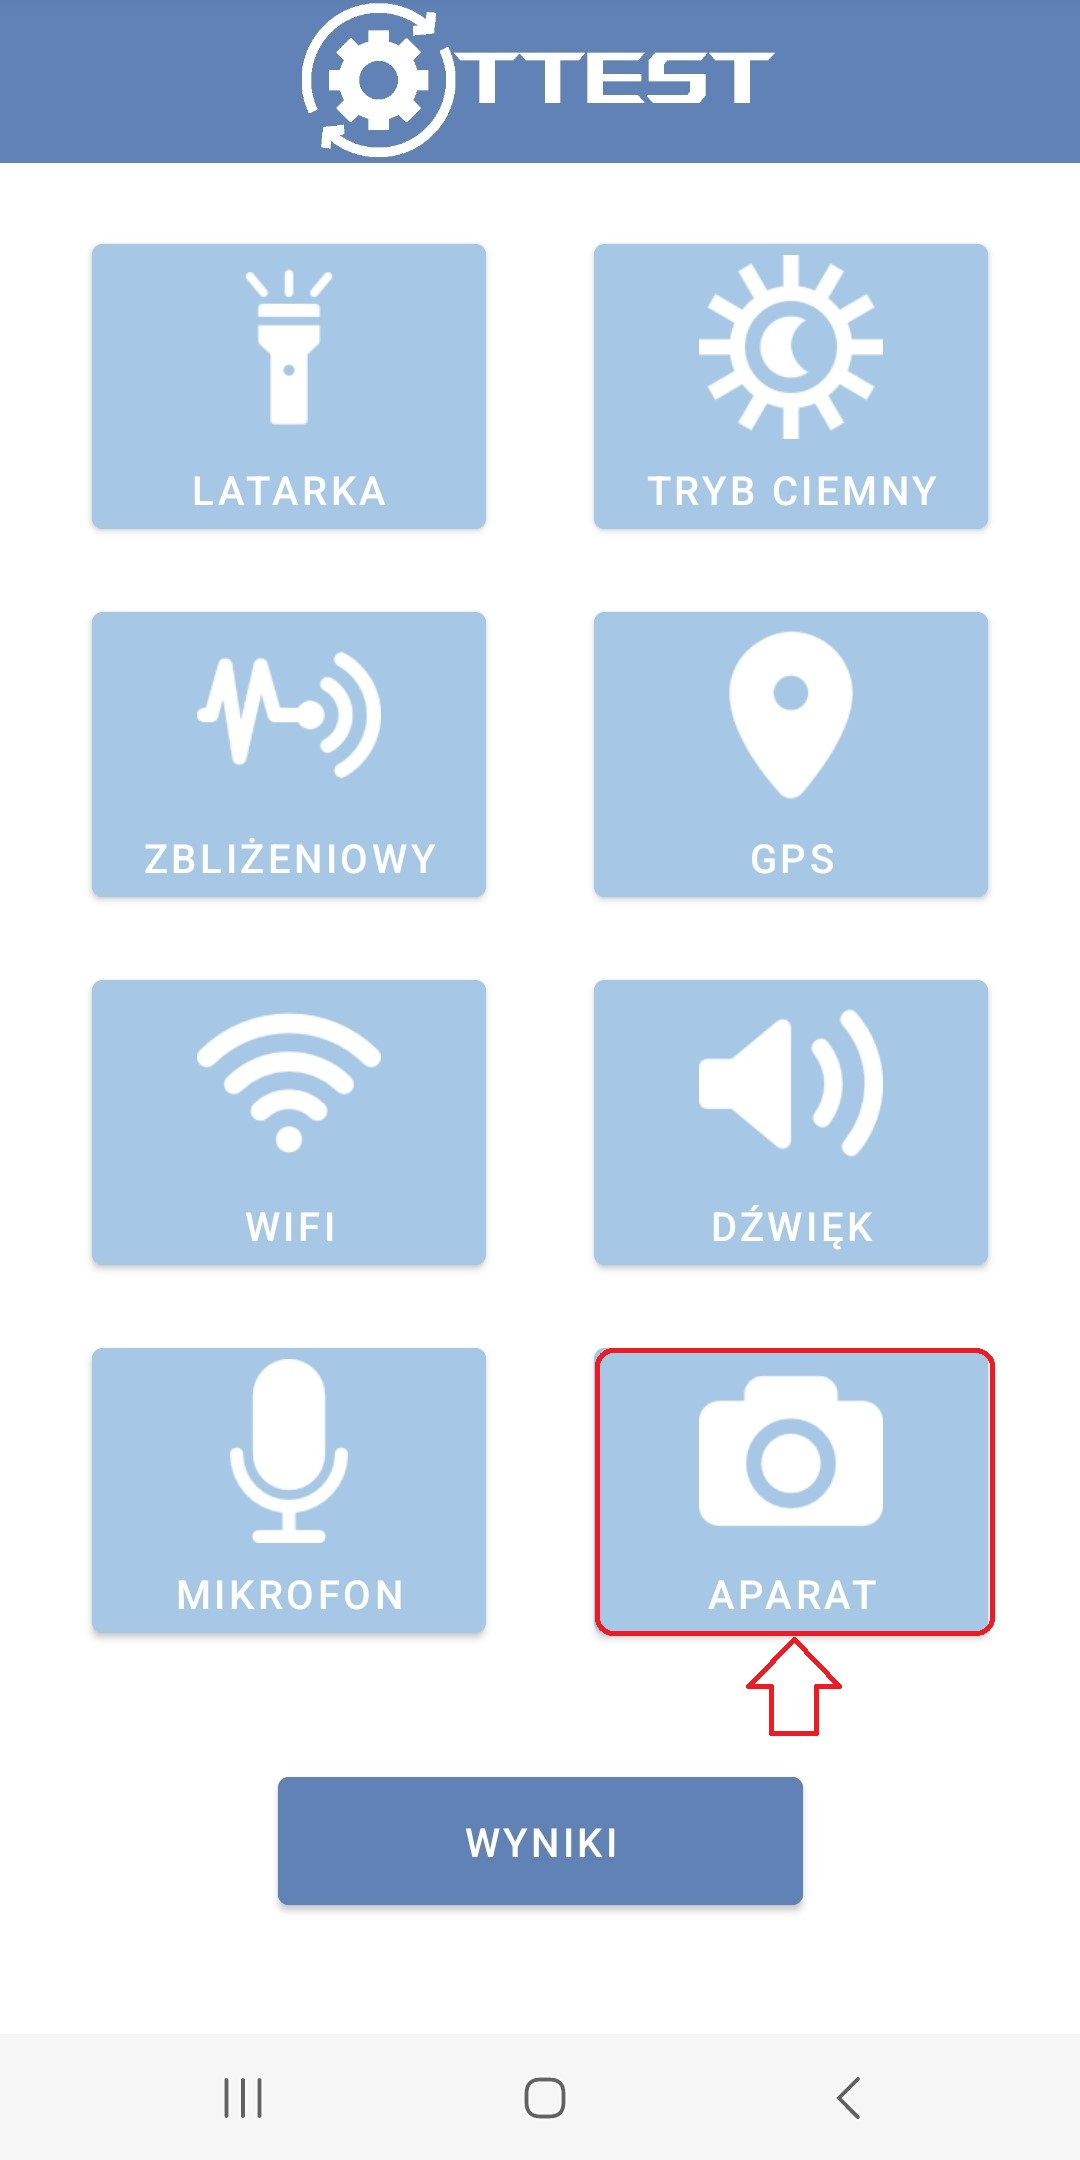
\includegraphics[angle=360, width=0.45\textwidth]{rys/punkt6/menu7}
		\caption{Wybór testu aparatu}
		\label{rys:menu7}
	\end{center}
\end{figure}

\newpage


Po przejściu na stronę z testem dostrzegamy że na środku znajduję się przycisk z napisem - "Zrób zdjęcie". Rysunek \ref{rys:aparat} prezentuję przycisk uruchamiający test aparatu.

\begin{figure}[!hbt]
	\begin{center}
		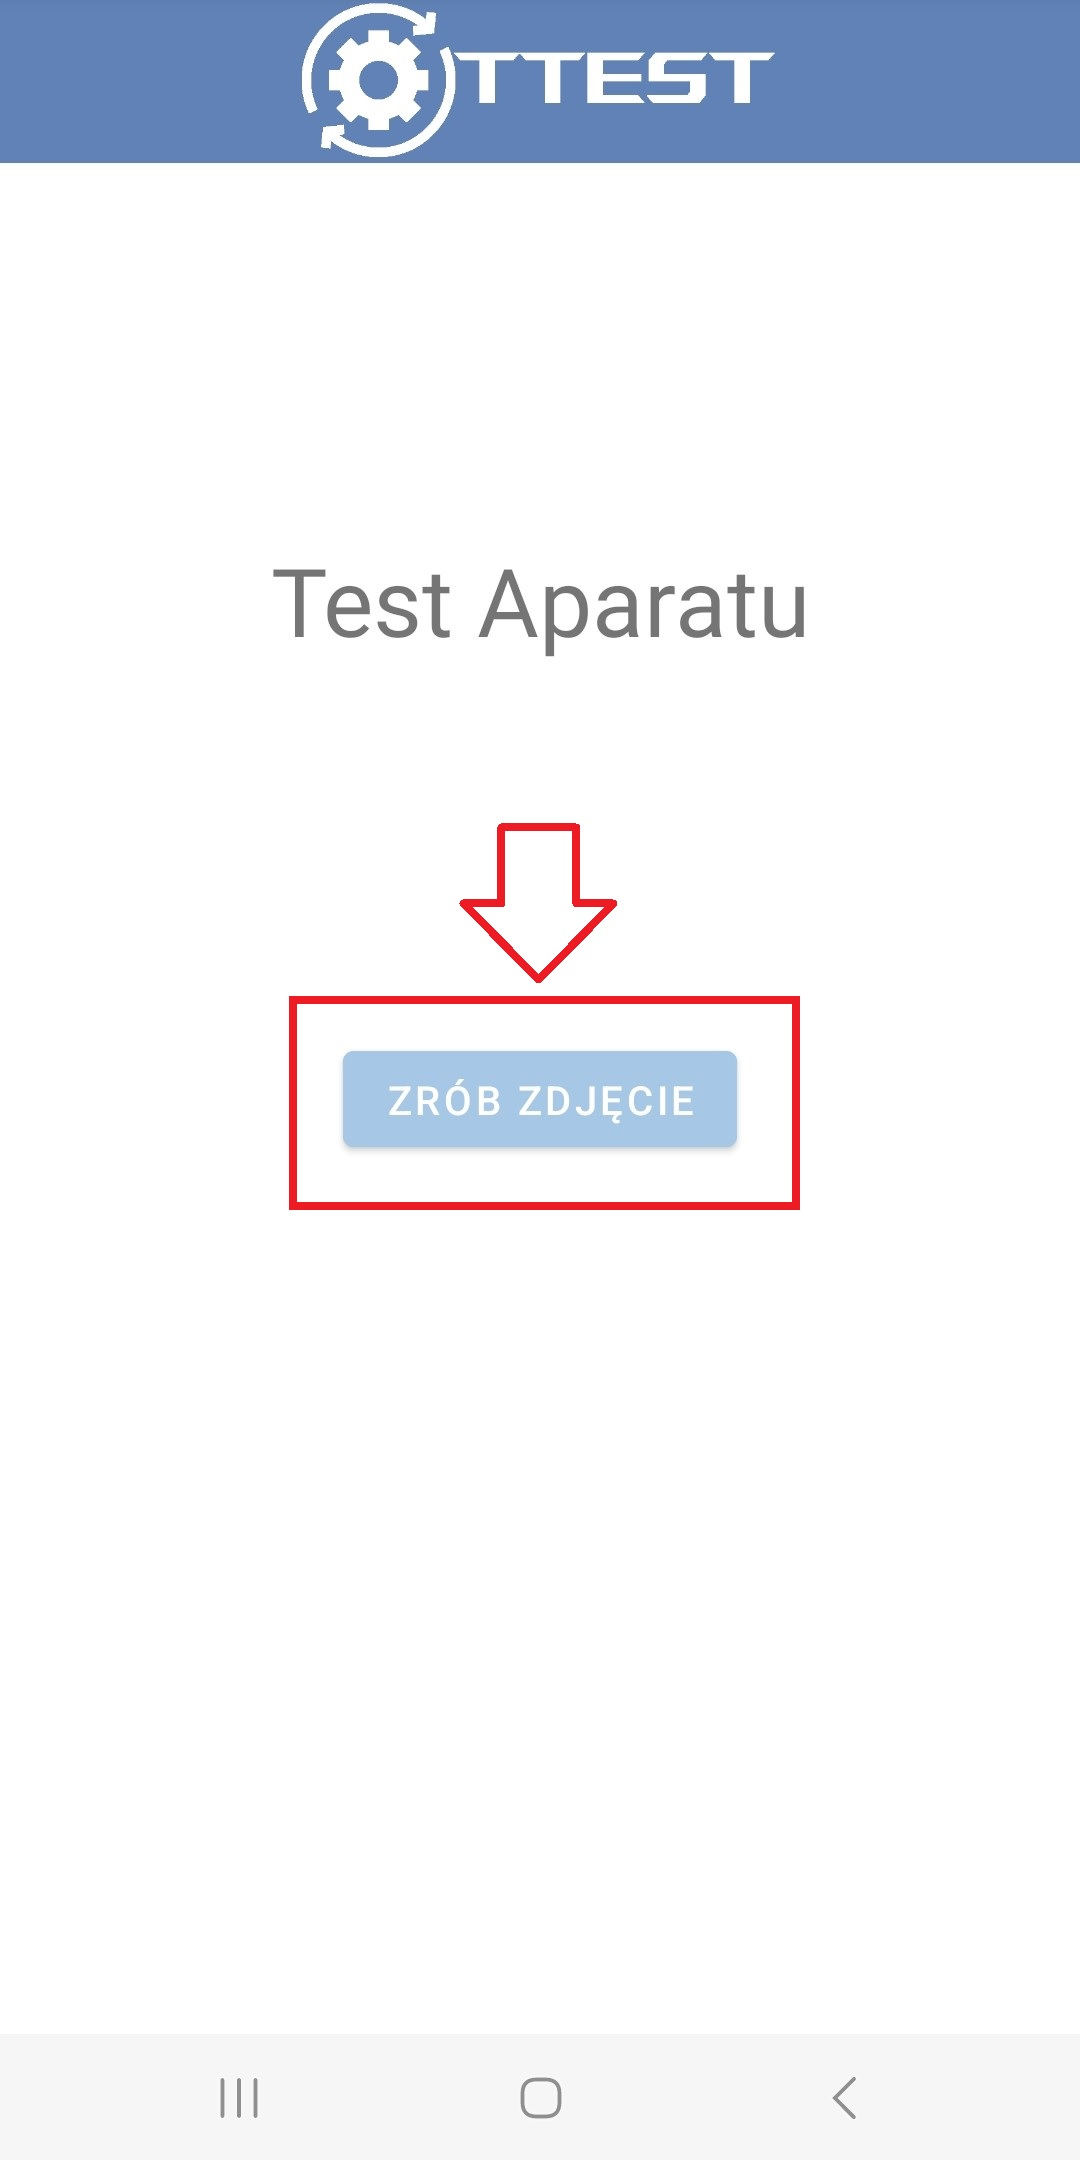
\includegraphics[angle=360, width=0.45\textwidth]{rys/punkt6/aparat}
		\caption{Strona testowa aparatu}
		\label{rys:aparat}
	\end{center}
\end{figure}

\newpage


Gdy naciśniemy przycisk zostaje uruchomiony aparat i możemy wykonać zdjęcie poprzez kliknięcie białego kółka znajdującego się u dołu ekranu. \\
Rysunek \ref{rys:aparat1} prezentuję test aparatu.

\begin{figure}[!hbt]
	\begin{center}
		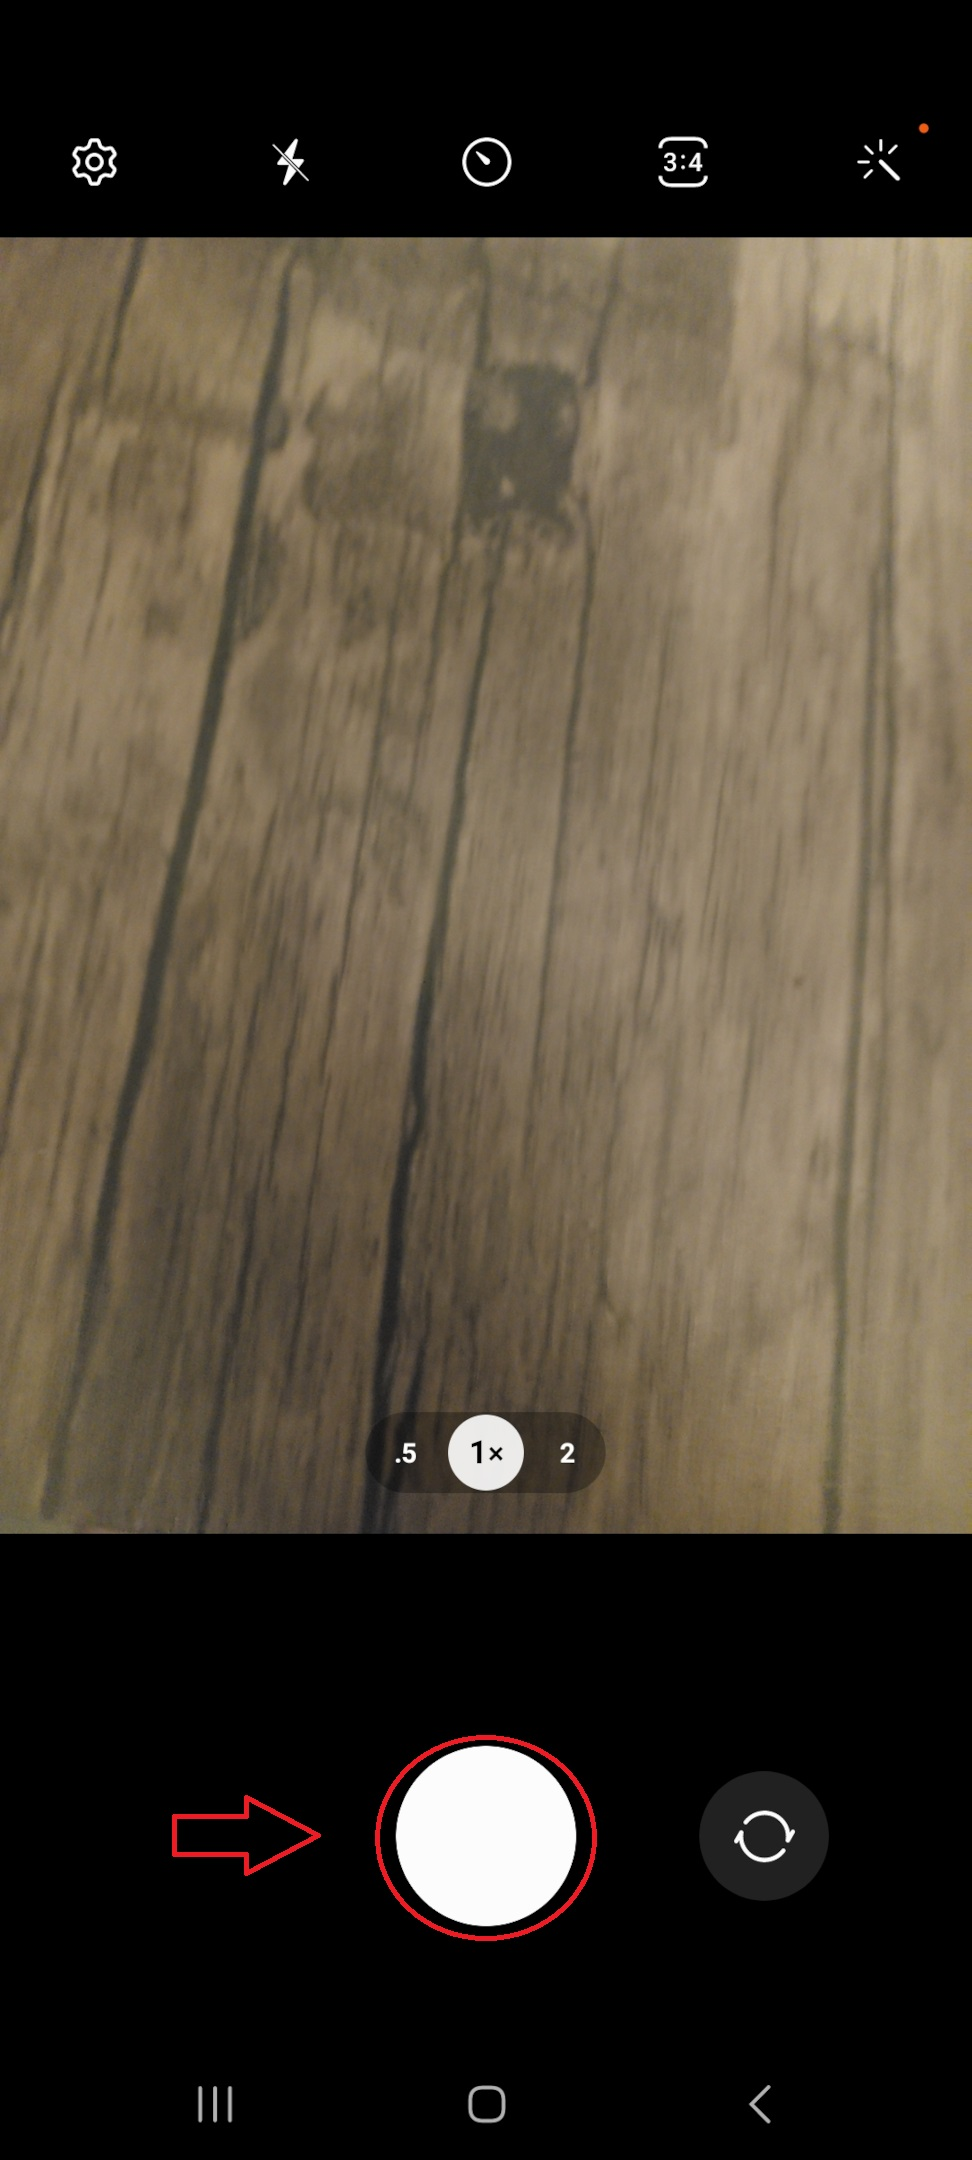
\includegraphics[angle=360, width=0.45\textwidth]{rys/punkt6/aparat1}
		\caption{Wykonanie zdjęcia- test aparatu}
		\label{rys:aparat1}
	\end{center}
\end{figure}

\newpage


Po wykonaniu zdjęcia, możemy ponowić próbę lub zakończyć test klikając przycisk: "OK". Rysunek \ref{rys:aparat2} przedstawia zrzut ekranu potwierdzający pomyślny przebieg testu.

\begin{figure}[!hbt]
	\begin{center}
		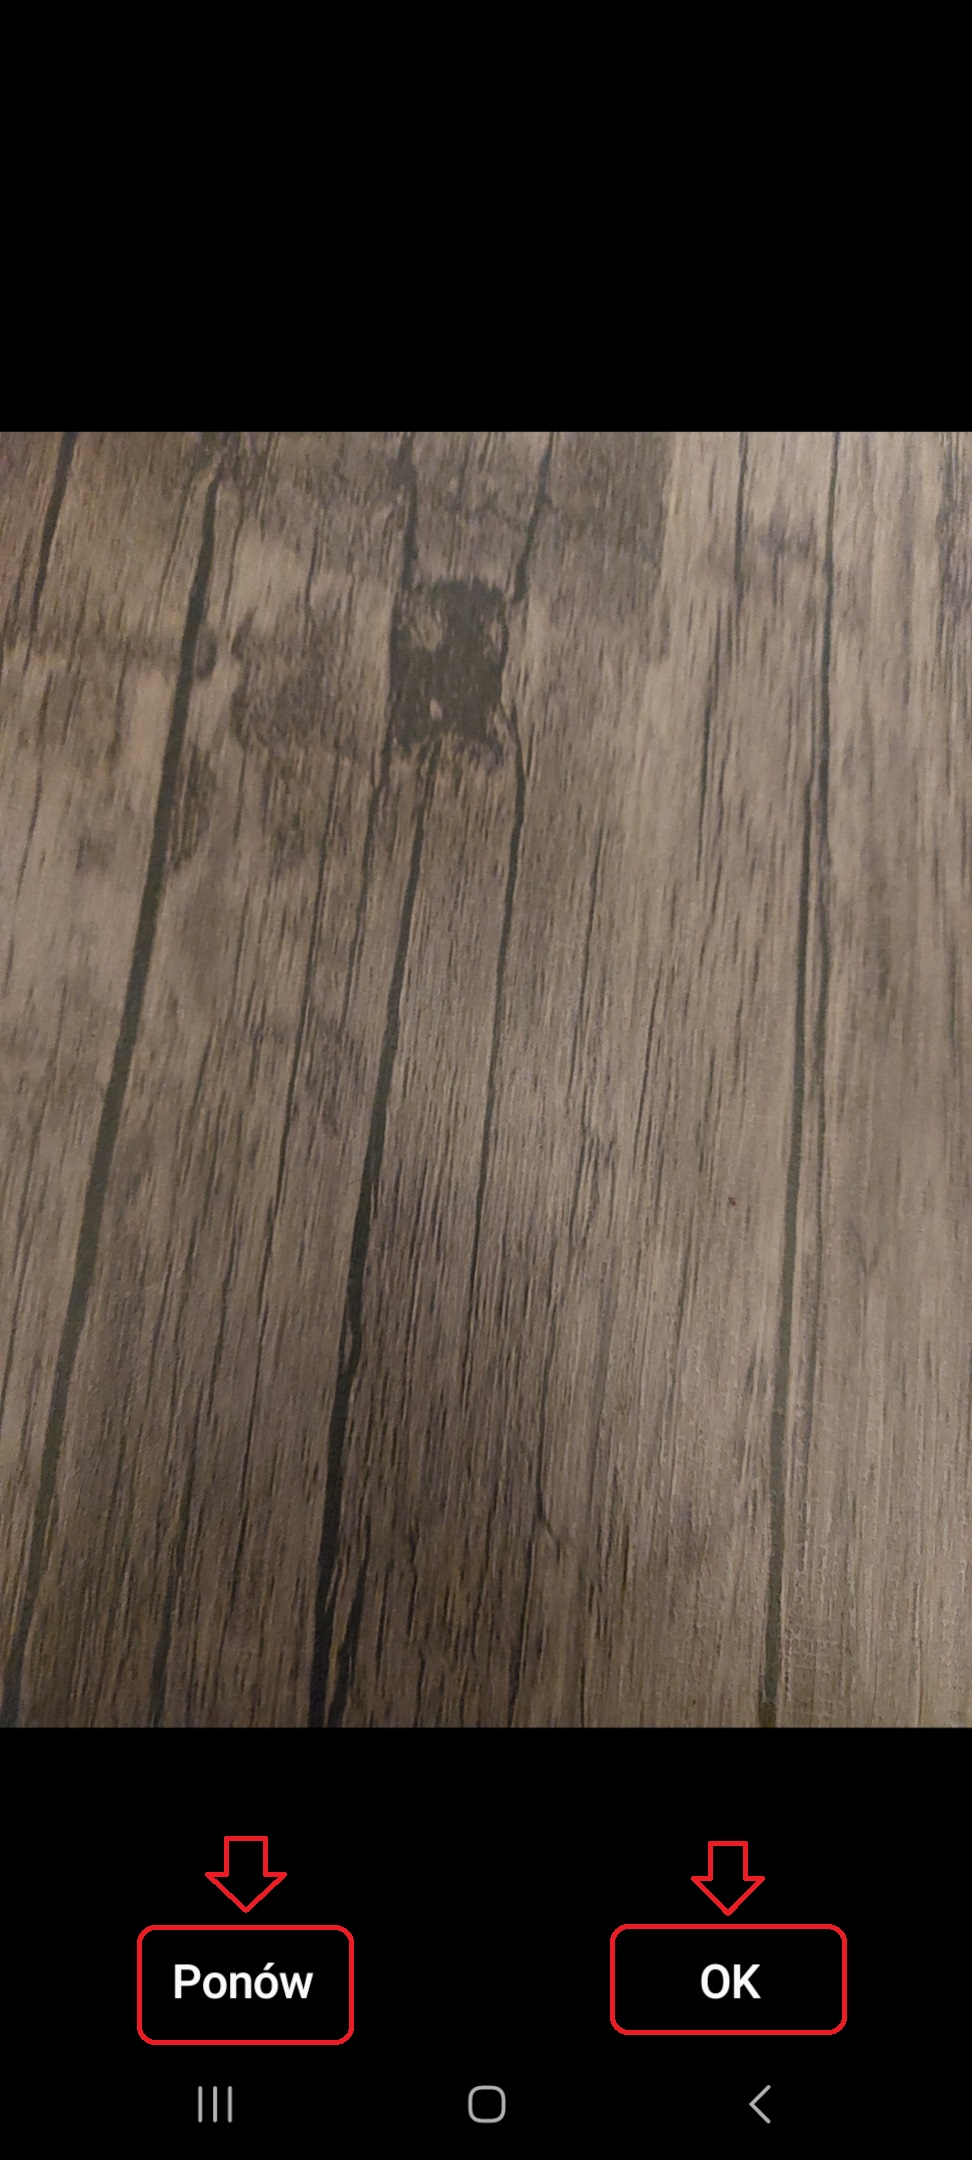
\includegraphics[angle=360, width=0.45\textwidth]{rys/punkt6/aparat2}
		\caption{Wykonanie kolejnego zdjęcia lub koniec testu - test aparatu}
		\label{rys:aparat2}
	\end{center}
\end{figure}

\newpage


\subsection{Podsumowanie wszystkich testów}

\hspace{0.60cm}Aby przejść do wykonania podsumowania wszystkich testów, należy w menu głównym wybrać i kliknąć przycisk: "Wyniki" znajdujący się na samym dole pod wszystkimi testami. Rysunek \ref{rys:menu8} przedstawia kafelek który należy wybrać aby przejść do wyników.

\begin{figure}[!hbt]
	\begin{center}
		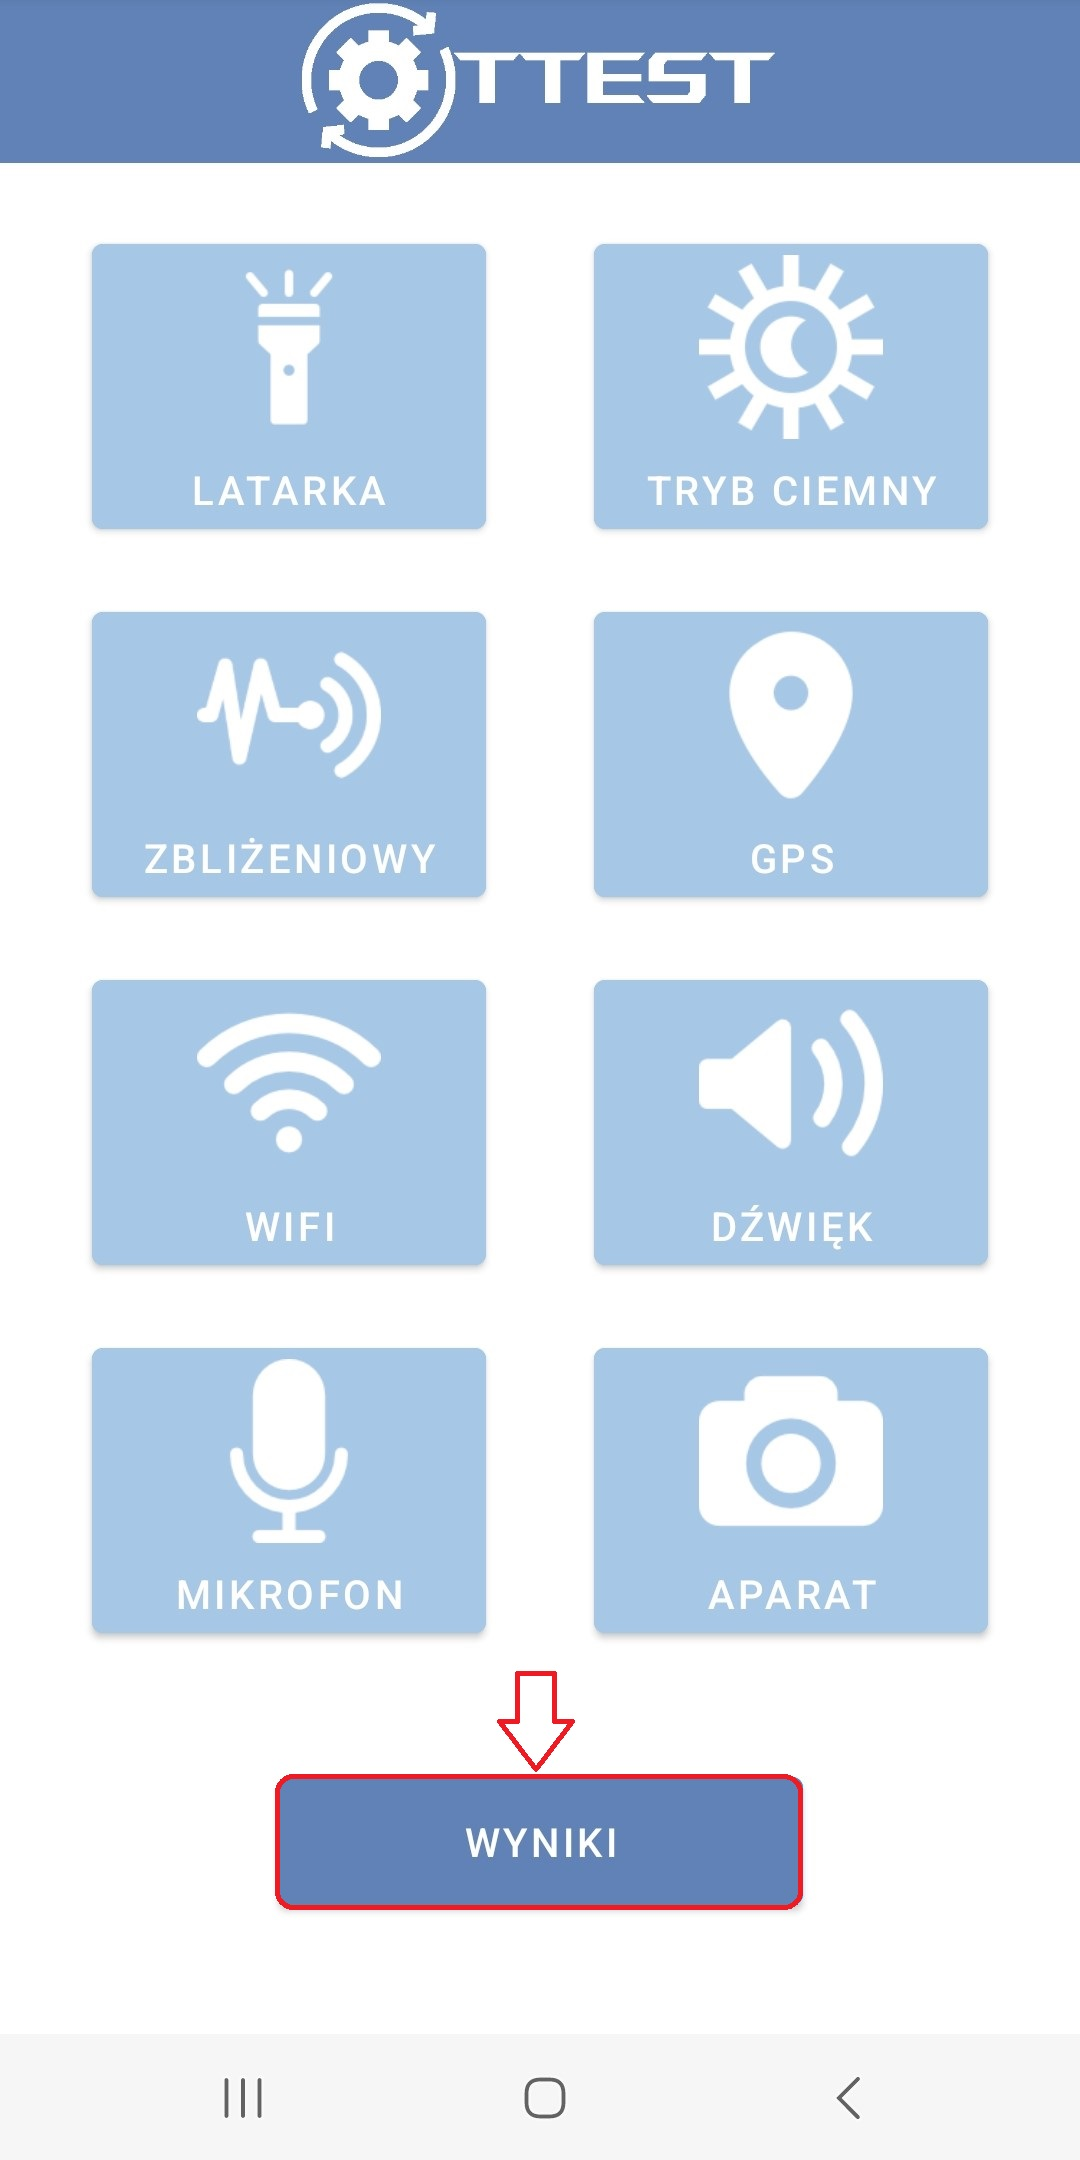
\includegraphics[angle=360, width=0.45\textwidth]{rys/punkt6/menu8}
		\caption{Przejście do sekcji "Wyniki"}
		\label{rys:menu8}
	\end{center}
\end{figure}

\newpage


Po przejściu na stronę z wynikami dostrzegamy że na samej górze po lewej stronie podany jest marka oraz model naszego telefonu. Co więcej na środku wymienione zostały wszystkie testy, które aplikacja posiada. Naszym zadaniem jest zaznaczyć odpowiednią odpowiedź w zależności czy test odbył się pomyślnie - odpowiedź "Tak" lub w przypadku gdy test nie przeszedł pomyślnie - odpowiedź "Nie". Następnym krokiem jest naciśnięcie przycisku "Podsumuj", który zsumuje wszystkie testy. Rysunek \ref{rys:wyniki} prezentuję podsumowanie testów.

\begin{figure}[!hbt]
	\begin{center}
		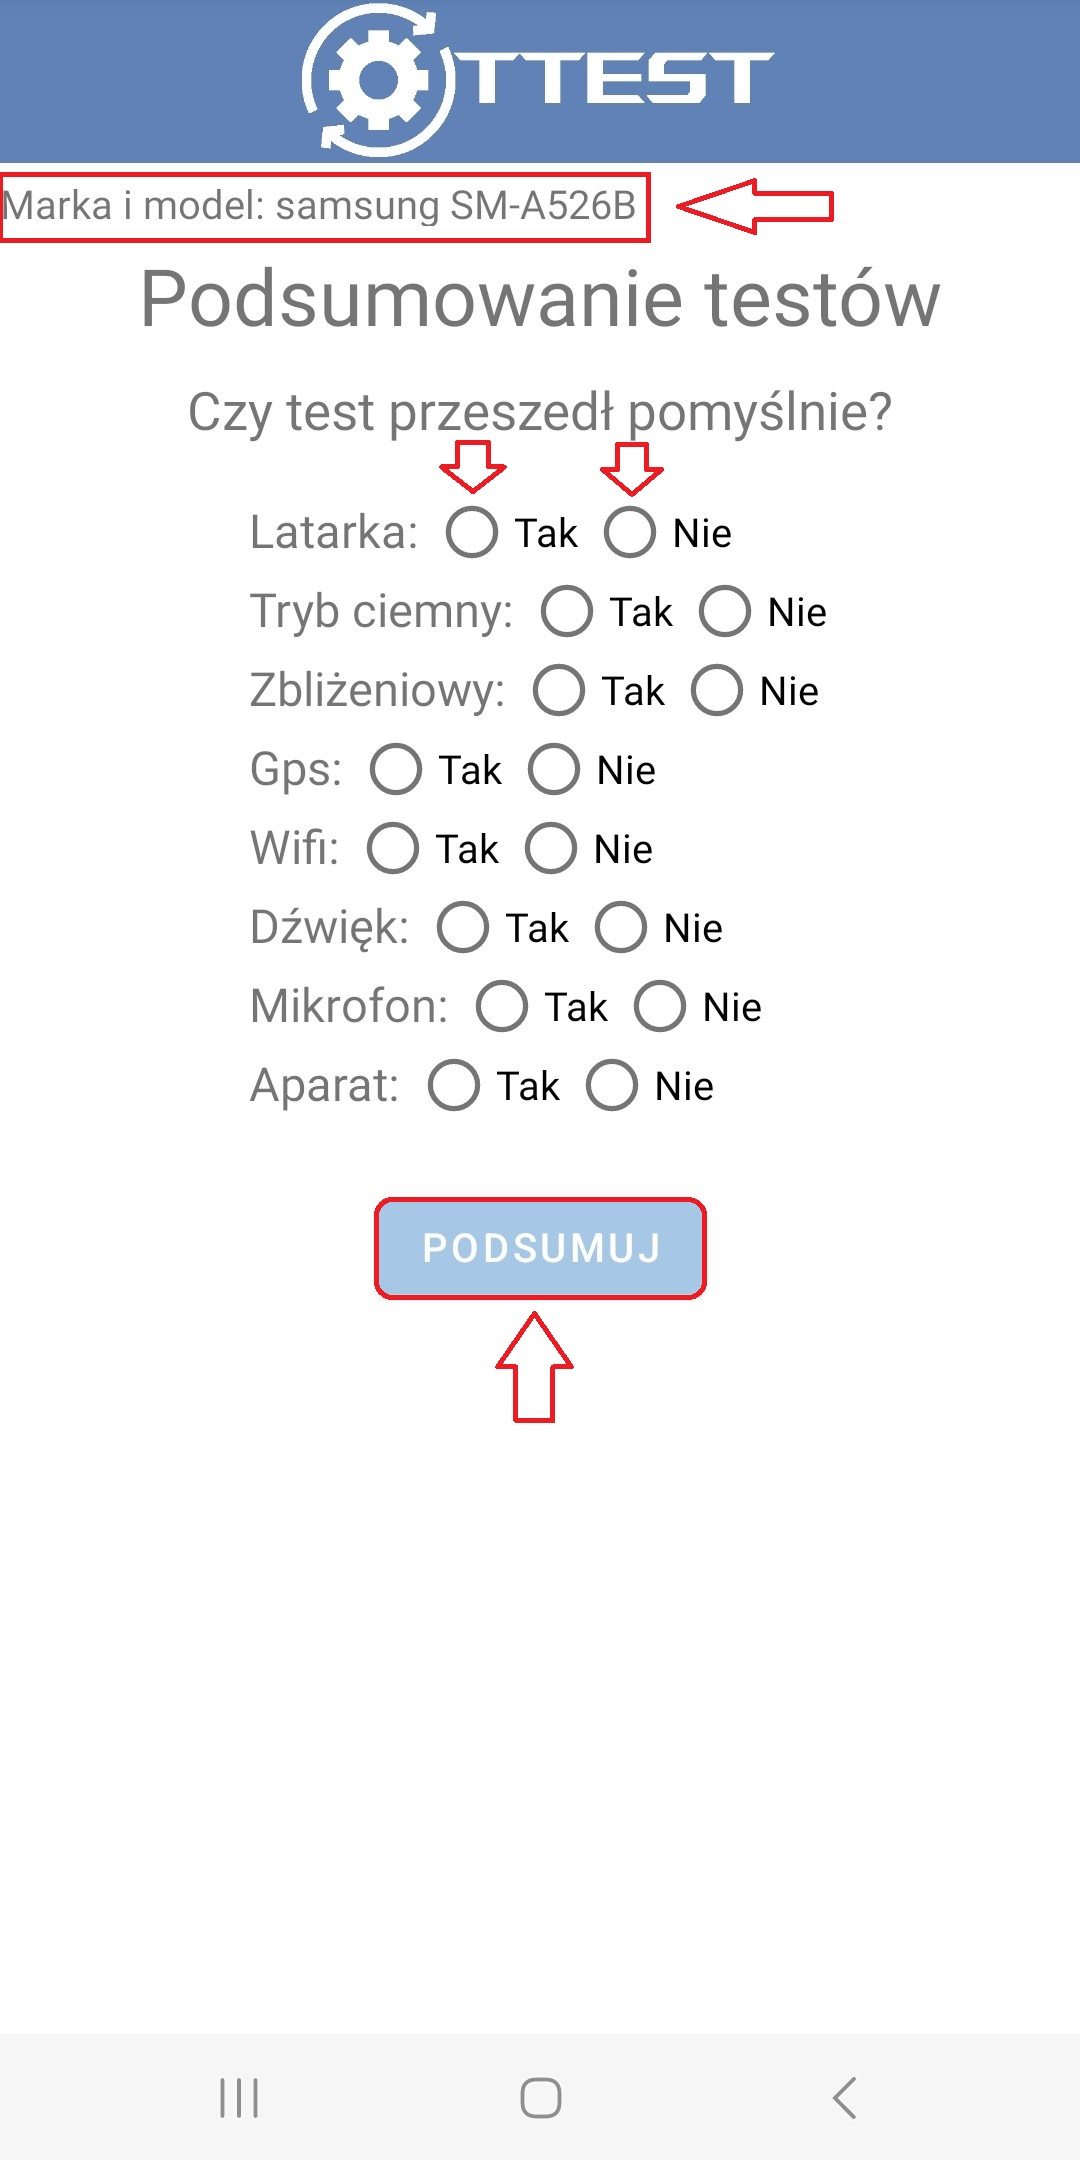
\includegraphics[angle=360, width=0.48\textwidth]{rys/punkt6/wyniki}
		\caption{Strona z podsumowaniem testów.}
		\label{rys:wyniki}
	\end{center}
\end{figure}

W przypadku gdy wszystkie testy przebiegły pomyślnie zostaną one wypisane zieloną czcionką, u dołu ekranu pod przyciskiem podsumowującym. \\
Rysunek \ref{rys:wyniki1} prezentuję podsumowanie wszystkich testów, które przebiegły pomyślnie.

\newpage


\begin{figure}[!hbt]
	\begin{center}
		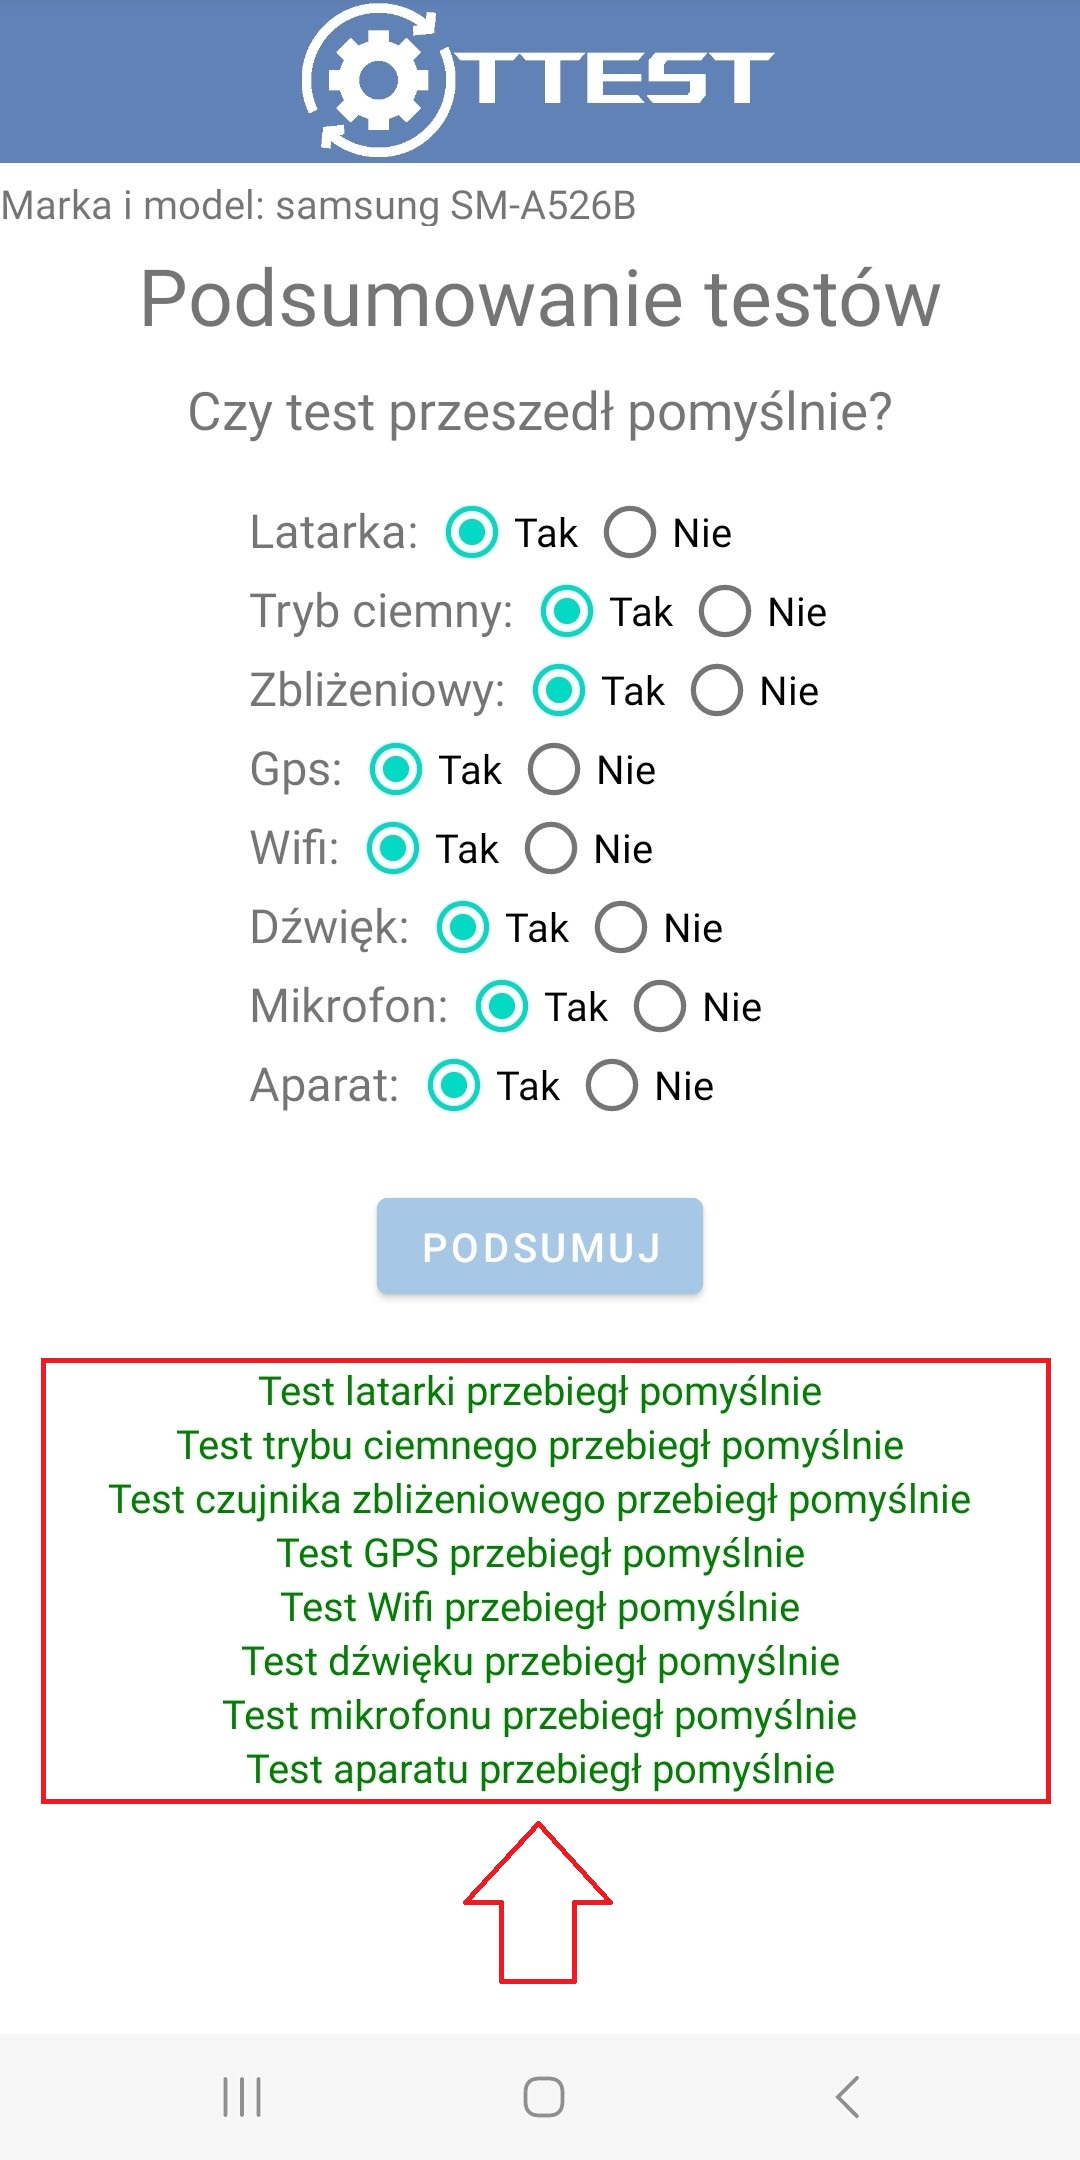
\includegraphics[angle=360, width=0.31\textwidth]{rys/punkt6/wyniki1}
		\caption{Podsumowanie wszystkich testów, które przebiegły pomyślnie}
		\label{rys:wyniki1}
	\end{center}
\end{figure}

Jeżeli wszystkie testy nie przebiegły pomyślnie zostaną one wypisane czerwoną czcionką, u dołu ekranu pod przyciskiem podsumowującym. Rysunek \ref{rys:wyniki2} prezentuję podsumowanie wszystkich testów, które nie przebiegły pomyślnie.

\begin{figure}[!hbt]
	\begin{center}
		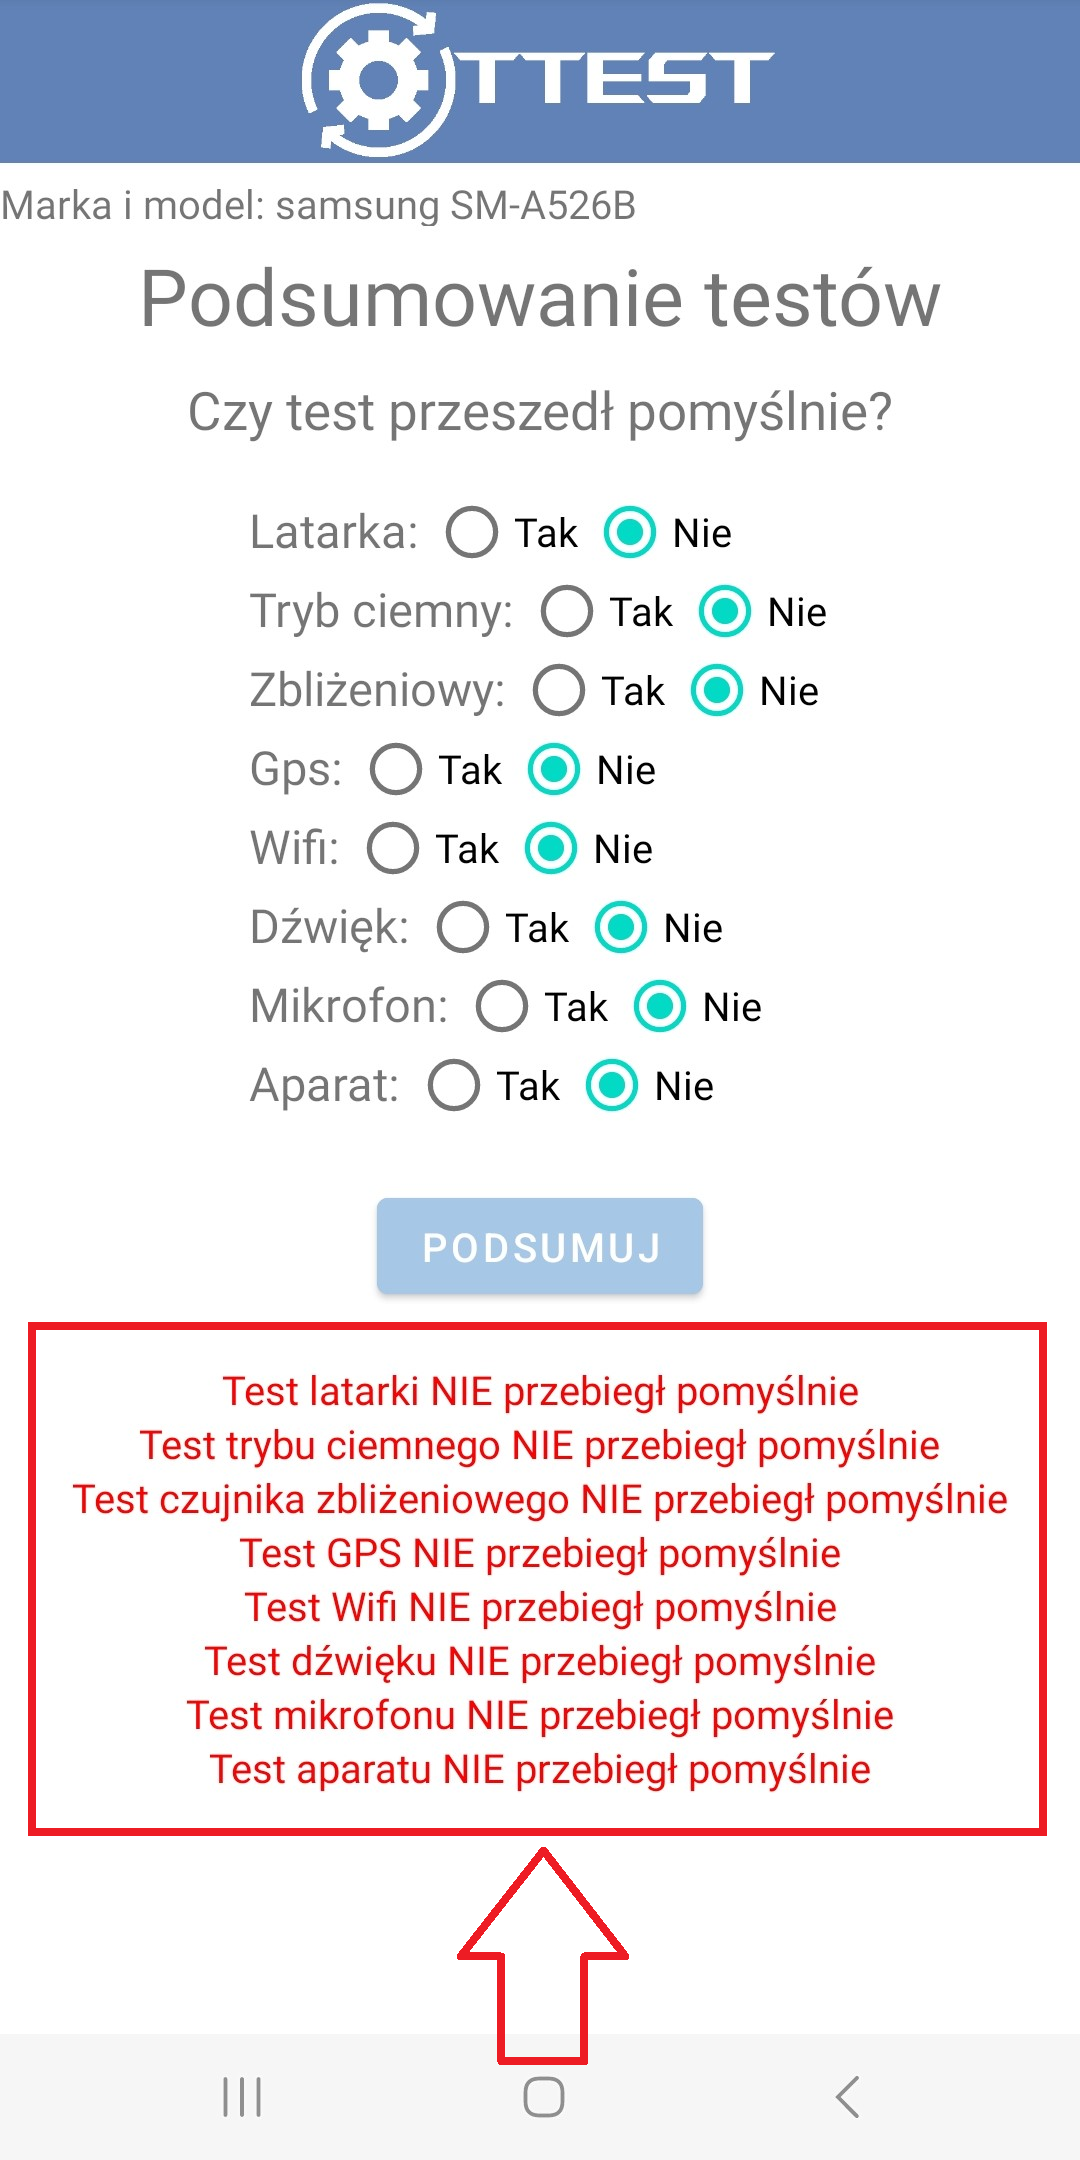
\includegraphics[angle=360, width=0.31\textwidth]{rys/punkt6/wyniki2}
		\caption{Podsumowanie wszystkich testów, które nie przebiegły pomyślnie}
		\label{rys:wyniki2}
	\end{center}
\end{figure}












